\documentclass[twoside]{book}
\usepackage{lectures}
\hypersetup{pdftitle={Comparison geometry}}
\makeindex

\begin{document}
\title{\tt What is differential geometry:\\
curves and surfaces}
\author{\tt Anton Petrunin and \\ \tt Sergio Zamora Barrera}
\date{}
\maketitle
\thispagestyle{empty}

\chapter{Review}

Here we state and discuss results from different branches of mathematics which were used further in the book.
The reader is not expected to know proofs of these statements, but it is better to check that his intuition agrees with each.  

\section{Metric spaces}

\emph{Metric} is a function that returns a real value $\Dist(x,y)$ for any pair $x,y$ in a given nonempty set $\mathcal X$  and satisfies the following axioms for any triple $x,y,z$:
\begin{enumerate}[(a)]
\item\label{def:metric-space:a} Positiveness: 
$$\Dist(x,y)\ge 0.$$
\item\label{def:metric-space:b} $x=y$ if and only if 
$$\Dist(x,y)=0.$$
\item\label{def:metric-space:c} Symmetry: $$\Dist(x, y) = \Dist(y, x).$$
\item\label{def:metric-space:d} Triangle inequality: 
$$\Dist(x, z) \le \Dist(x, y) + \Dist(y, z).$$
\end{enumerate}

A set with a metric is called \emph{metric space} and the elements of the set are called \emph{points}.

\parbf{Shortcut for distance.}
Usually we consider only one metric on a set, therefore we can denote the metric space and its underlying set by the same letter, say $\mathcal X$.
In this case we also use a shortcut notations $|x-y|$ or  $|x-y|_\mathcal X$ for the \emph{distance $\Dist(x,y)$ from $x$ to $y$ in $\mathcal X$}.
For example, the triangle inequality can be written as 
$$|x-z|_{\mathcal X}\le |x-y|_{\mathcal X}+|y-z|_{\mathcal X}.$$

\parbf{Examples.}
Euclidean space and plane as well as real line will be the most important examples of metric spaces for us.
In these examples the introduced notation $|x-y|$ for the distance from $x$ to $y$ has perfect sense as a norm of the vector $x-y$.
However, in general metric space the expression $x-y$ has no sense, but anyway we use expression $|x-y|$ for the distance.

If we say \emph{plane} or \emph{space} we mean \emph{Eucledean} plane or space.
However the plane (as well as the space) admits many other metrics, for example the so called Manhattan metric from the following exercise.

\begin{thm}{Exercise}
Consider the function
$$\Dist(p,q)=|x_p-x_q|+|y_p-y_q|,$$
where $p=(x_p,y_p)$ and $q=(x_q,y_q)$ are points in the coordinate plane $\RR^2$.
Show that $\Dist$ is a metric on $\RR^2$.
\end{thm}

Let us mention another example: the \emph{discrete space} --- arbitrary nonempty set $\mathcal X$ with the metric defined as $|x\z-y|_{\mathcal X}=0$ if $x=y$ and $|x-y|_{\mathcal X}=1$ otherwise.

\parbf{Subspaces.}
Any subset of a metric space is also a metric space, by restricting the original metric to the subset;
the obtained metric space is called a \emph{subspace}.
In particular, all subsets of Euclidean space are metric spaces.

\parbf{Balls.}
Given a point $p$ in a metric space ${\mathcal X}$ and a real number $R\ge 0$, the set of points $x$ on the distance less then $R$ (or at most $R$) from $p$ is called open (or correspondingly closed) ball of radius $R$ with center at $p$.
The \emph{open ball} is denoted as $B(p,R)$ or $B(p,R)_{\mathcal X}$;
the second notation is used if we need to emphasize that the ball lies in the metric space $\mathcal X$.
Formally speaking
\[B(p,R)=B(p,R)_{\mathcal X}=\set{x\in \mathcal X}{|x-p|_{\mathcal X}< R}.\]
Analogously, the \emph{closed ball} is denoted as $\bar B[p,R]$ or $\bar B[p,R]_{\mathcal X}$ and
\[\bar B[p,R]=\bar B[p,R]_{\mathcal X}=\set{x\in \mathcal X}{|x-p|_{\mathcal X}\le R}.\]

\begin{thm}{Exercise}\label{ex:B2inB1}
Let $\mathcal X$ be a metric space.
\begin{enumerate}[(a)]
\item Show that if $\bar B[p,2]\subset \bar B[q,1]$
for some points $p,q\in \mathcal X$, then $\bar B[p,2]= \bar B[q,1]$.
\item Construct a metric space $\mathcal X$ with two points $p$ and $q$ such that
$B(p,\tfrac32)\subset B(q,1)$ and the inclusions is strict.
\end{enumerate}

\end{thm}



\section{Continuity}

In this section we will extend standard notions from calculus to the metric spaces.

\begin{thm}{Definition}
 Let ${\mathcal X}$ be a metric space.
A sequence of points $x_1, x_2, \ldots$ in ${\mathcal X}$ is called \emph{convergent}\index{convergent}
if there is 
$x_\infty\in {\mathcal X}$ such that $|x_\infty -x_n|\to 0$ as $n\to\infty$.  
That is, for every $\eps > 0$, there is a natural number $N$ such that for all $n \ge N$, we have $$|x_\infty-x_n| < \eps.$$

In this case we say that the sequence $(x_n)$ \emph{converges} to $x_\infty$, 
or $x_\infty$ is the \emph{limit} of the sequence $(x_n)$.
Notationally, we write $x_n\to x_\infty$ as $n\to\infty$
or $x_\infty=\lim_{n\to\infty} x_n$.
\end{thm}

\begin{thm}{Definition}
Let ${\mathcal X}$ and ${\mathcal Y}$ be metric spaces.
A map $f\:{\mathcal X}\to {\mathcal Y}$ is called \emph{continuous} if for any convergent sequence $x_n\to x_\infty$ in ${\mathcal X}$,
%the sequence $y_n\z=f(x_n)$ converges to $y_\infty=f(x_\infty)$ in ${\mathcal Y}$.
we have $f(x_n) \to f(x_\infty)$ in ${\mathcal Y}$.

Equivalently, $f\:{\mathcal X}\to {\mathcal Y}$ is continuous if for any $x\in {\mathcal X}$ and any $\eps>0$,
there is $\delta>0$ such that 
$$|x-x'|_{\mathcal X}<\delta\ \text{ implies }\ |f(x)-f(x')|_{\mathcal Y}<\eps.$$
%$$|x-x'|_{\mathcal X}<\delta\ \Rightarrow\ |f(x)-f(x')|_{\mathcal Y}<\eps.$$

\end{thm}

\begin{thm}{Exercise}
Let ${\mathcal X}$ and ${\mathcal Y}$ be metric spaces $f\:{\mathcal X}\to {\mathcal Y}$ is \emph{distance non-expanding map}; that is, 
\[|f(x)-f(x')|_{\mathcal Y}\le |x-x'|_{\mathcal X}\]
for any $x,x'\in \mathcal X$.
Show that $f$ is continuous.
\end{thm}

\begin{thm}{Definition}
Let ${\mathcal X}$ and ${\mathcal Y}$ be metric spaces.
A continous bijection $f\:{\mathcal X}\to {\mathcal Y}$ 
is called a \emph{homeomorphism}\index{homeomorphism} 
if its inverse $f^{-1}\:{\mathcal Y}\z\to {\mathcal X}$ is also continuous.

If there exists a homeomorphism $f\:{\mathcal X}\to {\mathcal Y}$,
we say that ${\mathcal X}$ is \emph{homeomorphic}\index{homeomorphic} to ${\mathcal Y}$,
or  $\mathcal X$ and ${\mathcal Y}$ are \emph{homeomorphic}.
\end{thm}

If a metric space $\mathcal X$ is homeomorphic to a known space, for example plane, sphere, disc, circle and so on,
we may also say that $\mathcal X$ is a \emph{topological} plane, sphere, disc, circle and so on.

\begin{thm}{Definition}
A subset $A$ of a metric space $\mathcal{X}$ is called \emph{closed}\index{closed set} if whenever a sequence $(x_n)$ of points from $A$ converges in $\mathcal{X}$, we have that $\lim_{n\to\infty} x_n \in A$.

A set $\Omega \subset \mathcal{X}$ is called \emph{open}\index{open set} if for any $z\in \Omega$, 
there is $\eps>0$ such that $B(z,\eps)\subset\Omega$.
\end{thm}

An open set $\Omega$ that contains a given point $p$ is called \emph{neighborhood of $p$}.

\begin{thm}{Exercise}
Let $Q$ be a subset of a metric space $\mathcal{X}$.
Show that $A$ is closed if and only if its complement $\Omega=\mathcal{X}\backslash Q$ is open.
\end{thm}

\chapter{Definitions}


\section*{Simple curves}

In the following definition we use the notion of \emph{metric space} which is discussed in Appendix~\ref{app:metric-spcaes}.
The Euclidean plane and space are the main examples of metric spaces that one should keep in mind. 

Recall that that a bijective continuous map $f\:X\to Y$ between subsets of some metric spaces is called \emph{homeomorphism} if its inverse $f^{-1}\:Y\z\to X$ is continuous.  

\begin{thm}{Definition} 
A connected subset $\gamma$ in a metric space is called a \emph{simple curve} if it is \emph{locally} homeomorphic to a real interval; that is, any point $p\in\gamma$ has a neighborhood $U\ni p$ such that the intersection
$U\cap \gamma$ is homeomorphic to an open real interval.
\end{thm}

It turns out that any curve can be \emph{parameterized} by an open real interval or a circle.
That is, for any curve $\gamma$ there is a homeomorphism $(a,b)\to\gamma$ or $\SS^1\to\gamma$ 
where $\SS^1$ denotes the unit circle; that is 
\[\SS^1=\set{(x,y)\in\RR^2}{x^2+y^2=1}.\]
We omit a proof of this statement; it is not hard, but would take us away from the subject.
We hope however that this statement is intuitively obvious. % a formal proof can be found in???.

Curves that admit a parametrization by a circle are called \emph{closed}.
The subsets of curves bounded from one or two sides by points are called \emph{curves with endpoints}.
If it has two endpoints, then it is called \emph{arc}; note that any arc can be parameterized by a closed interval.
A curve as well as a curve with endpoint(s) can be regarded as a curve;
if we need to emphasize that we work with a genuine curve we may say a \emph{curve without endpoints}.


A parametrization describes a curve completely.
Often we will denote a curve and its parametrization by the same letter;
for example, we may say a plane curve $\gamma$ is given with a parametrization $\gamma\:(a,b)\to \RR^2$.
Note however that any curve admits many different parametrization. 

\begin{thm}{Exercise}\label{ex:9}
Find a continuous injective map $\gamma\:(0,1)\to\RR^2$ such that its image is not a simple curve.
\end{thm}


\section*{Parameterized curves}

A \emph{parameterized curve} is defined as a continuous map $\gamma$ from a circle or a real interval (open, closed or semi-open) to a metric space. 
For a parameterized curve we do not assume that $\gamma$ is injective; in other words a parameterized curve might have \emph{self-intersections}.

If we say \emph{curve} it means we do not want to specify whether it is a parameterized curve or a simple curve.

If the domain of a parameterized curve is the closed unit interval $[0,1]$, then it is also called a \emph{path}.
If in addition $p=\gamma(0)=\gamma(1)$, then $\gamma$ is called a loop;
the point $p$ in this case is called \emph{base} of the loop.

\begin{thm}{Advanced exercise}
Let $X$ be a subset of the plane.
Suppose that two distinct points $p,q\in X$ can be connected by a path in $X$.
Show that there is a simple arc in~$X$ connecting $p$ to $q$.
\end{thm}

\section*{Smooth curves}

A curve in the Euclidean space or plane, is called \emph{space} or \emph{plane curve} correspondingly.

A parameterized space curve can be described by its coordinate functions 
\[\gamma(t)=(x(t),y(t),z(t)).\]
Plane curves can be considered as a partial case of space curves with $z(t)\equiv 0$.

Recall that a real-to-real function is called \index{smooth function}\emph{smooth} if its derivatives of all orders are defined everywhere in the domain of definition.  
If each of the coordinate functions $t\mapsto x(t),t\mapsto y(t)$ and $t\mapsto z(t)$ of the space curve $\gamma$ is a smooth, then the parameterized curve is called \index{smooth curve}\emph{smooth}.

If the \emph{velocity vector} 
\[\gamma'(t)=(x'(t),y'(t),z'(t))\] 
does not vanish at all points, then the parameterized curve $\gamma$ is called \emph{regular}.

A simple space curve is called \emph{smooth and regular} if it admits a smooth and regular parametrization.
Regular smooth curves are among the main objects in differential geometry;
colloquially, the term \emph{smooth curve} often used as a shortcut for \emph{smooth regular curve}. 

\begin{thm}{Exercise}\label{ex:L-shape}
Note that the function 
\[f(t)=
\begin{cases}
0&\text{if}\ t\le 0,
\\
\frac{t}{e^{1\!/\!t}}&\text{if}\ t> 0.
\end{cases}
\]
is smooth. Indeed, the existence of all derivatives $f^{(n)}(x)$ at $x\ne 0$ is evident and direct calculations show that $f^{(n)}(0)=0$ for any $n$.

Show that $\gamma(t)=(f(t),f(-t))$ gives a smooth parametrization of a simple curve formed by the union of two half-axis in the plane.

Show that any smooth parametrization of this curve has vanishing velocity vector at the origin.
Conclude that this curve is not regular and smooth;
that is, it does not admit a regular smooth parametrization.
\end{thm}


\begin{thm}{Exercise}\label{ex:cycloid}
Describe the set of real numbers $\ell $
such that the plane curve $\gamma_\ell (t)= (t+\ell \cdot \sin t,\ell \cdot \cos t)$, $t\in\RR$ is
\begin{enumerate}[(a)]
\item regular;
\item simple.
\end{enumerate}

\end{thm}

\section*{Periodic parametrization}
Note that any closed simple curve can be described as an image of a loop.
However, it is more natural to present it as a \emph{periodic} parameterized curve $\gamma\: \RR\to \mathcal{X}$; that is, such that $\gamma(t+\ell)=\gamma(t)$ for a fixed period $\ell$ and any $t$.
For example the unit circle in the plane can be described by $2{\cdot}\pi$-periodic parametrization $\gamma(t)=(\cos t,\sin t)$.

{

\begin{wrapfigure}{o}{17 mm}
\vskip-3mm
\centering
\includegraphics{mppics/pic-51}
\end{wrapfigure}

Any smooth regular closed curve can be described by a smooth regular loop.
But in general the closed curve that described by a smooth regular loop might fail to be smooth at its base; an example is shown on the diagram.

}

\section*{Implicitly defined curves}

Suppose $f\:\RR^2\to \RR$ is a smooth function; 
that is, all its partial derivatives defined in its domain of definition.
Let $\gamma\subset \RR^2$ be the set of solutions of the equation $f(x,y)=0$.

Assume $\gamma$ is connected.
According to implicit function theorem (\ref{thm:imlicit}), the set $\gamma$ is a smooth regular simple curve if $0$ is a \emph{regular value} of $f$.
In this case it means that the gradient $\nabla f$ does not vanish at any point $p\in \gamma$.
In other words, if $f(p)=0$, then  $\tfrac{\partial f}{\partial x}(p)\ne 0$ or $\tfrac{\partial f}{\partial y}(p)\ne 0$.

Similarly, assume $f,h$ is a pair of smooth functions defined in $\RR^3$.
The system of equations
\[\begin{cases}
   f(x,y,z)=0,
   \\
   h(x,y,z)=0.
  \end{cases}
\]
defines a regular smooth space curve if the set of solutions is connected and $0$ is a regular value of the map $F\:\RR^3\to\RR^2$ defined as
\[F\:(x,y,z)\mapsto (f(x,y,z),h(x,y,z)).\]
In this case it means that the gradients $\nabla f$ and $\nabla h$ are linearly independent at any point $p\in \gamma$.
In other words, the Jacobian matrix
\[
\begin{pmatrix}
\tfrac{\partial f}{\partial x}&\tfrac{\partial f}{\partial y}&\tfrac{\partial f}{\partial z}\\
\tfrac{\partial h}{\partial x}&\tfrac{\partial h}{\partial y}&\tfrac{\partial f}{\partial z}
\end{pmatrix}
\]
for the map $F\:\RR^3\to\RR^2$ has rank 2 at any $p$ such that $f(p)=h(p)=0$.

The described way to define a curve is called \emph{implicit};
if a curve is defined by its parametrization, we say that it is \emph{explicitly defined}.
While implicit function theorem guarantees the existence of regular smooth parametrizations, do not expect it to be in a closed form. 
When it comes to calculations, usually it is easier to work directly with implicit representation. 

\begin{thm}{Exercise}
Consider the set in the plane described by the equation
\[y^2=x^3.\]
Is it a simple curve? and if ``yes'', is it a smooth regular curve?
\end{thm}

\begin{thm}{Exercise}\label{ex:viviani}
Describe the set of real numbers $\ell$
such that the system of equations
\[\begin{cases}
x^2+y^2+z^2&=1
\\
x^2+\ell\cdot x+y^2&=0
\end{cases}\]
describes a smooth regular curve.
\end{thm}

\section*{Proper curves}

A parametrized curve $\gamma$ in a metric space $\mathcal{X}$ is called \emph{proper} if for any compact set $K$ the inverse image $\gamma^{-1}(K)$ is compact.

For example curve $\gamma(t)=(e^t,0,0)$ defined on whole real line is not proper.
Indeed the half-line $(-\infty,0]$ is not compact and it is the inverse image of unit closed ball around the origin.  

Note that any closed curve as well arc are proper curves since its parameter set is compact.

A simple curve is called proper if it admits a proper parametrization.
It turns out that simple curve is proper if and only if its image is a closed set.
In particular any implicitly defined plane or space curve is proper.
We omit the proof of this statement, but it is not hard. %??? ref

\begin{thm}{Exercise}\label{ex:proper-curve}
Use the Jordan's theorem (\ref{thm:jordan}) to show that any proper plane curve divides the plane in two connected components.  
\end{thm}




\chapter{Length}
 
Recall that a sequence 
\[a=t_0 < t_1 < \cdots < t_k=b.\]
is called a \emph{partition} of the interval $[a,b]$.

\begin{thm}{Definition}\label{def:length}
Let $\gamma\:[a,b]\to \mathcal{X}$ be a curve in a metric space.
The \emph{length}\index{length of curve} of $\gamma$ is defined as
\begin{align*}
\length \gamma
= 
\sup \{|\gamma(t_0)-\gamma(t_1)|&+|\gamma(t_1)-\gamma(t_2)|+\dots
\\
&\dots+|\gamma(t_{k-1})-\gamma(t_k)|\},
\end{align*}
where the supremum is taken over all partitions
\[a=t_0 < t_1 < \cdots < t_k=b.\]

The length of $\gamma$ is a nonnegative real number or infinity;
the curve $\gamma$ is called \emph{rectifiable}\index{rectifiable curve} if its length is finite. 

The length of a closed curve is defined as the length of the corresponding loop.
If a curve is defined on an open or semi-open interval, then its length is defined as the exact upper bound for lengths of all its arcs.
\end{thm}

Suppose $\gamma\:[a,b]\to \RR^3$ is a parameterized space curve.
For a partition $a=t_0 < t_1 < \cdots < t_k=b$, set $p_i=\gamma(t_i)$.
Then the polygonal line $p_0\dots p_k$ is called \emph{inscribed} in $\gamma$.
If $\gamma$ is closed, then $p_0=p_k$, so the inscribed polygonal line is also closed.

\begin{thm}{Exercise}\label{ex:integral-length-0}
Suppose $\gamma\:[a,b] \to\RR^3$ is a curve and the function $\phi : [c,d] \to [a,b]$ is an monotonic continuous and $\phi(c)=a$, $\phi(d)=b$.
Then the curve $\gamma \circ \phi$ is calle a 
\emph{reparametrization} of $\gamma$.
Show that 
\[\length (\gamma \circ \phi) = \length \gamma.\]

\end{thm}

Note that the length of space curve $\gamma$ can be defined as the exact upper bound of the lengths of polygonal lines $p_0\dots p_k$ \emph{inscribed} in $\gamma$.

\begin{thm}{Exercise}\label{ex:length-image}
Let $\alpha\:[0,1]\to\RR^3$ be a parametrization of a simple arc.
Suppose a path $\beta\:[0,1]\to\RR^3$ has the same image as $\alpha$;
that is, $\beta([0,1])=\alpha([0,1])$.
Show that 
\[\length \beta\ge \length \alpha.\]

\end{thm}

\begin{thm}{Exercise}\label{ex:integral-length}
Assume $\gamma\:[a,b]\to\RR^3$ is a smooth curve.
Show that
\begin{subthm}{ex:integral-length>} $\length \gamma\ge \int_a^b|\gamma'(t)|\cdot dt$,
\end{subthm}

\begin{subthm}{ex:integral-length<} $\length \gamma\le \int_a^b|\gamma'(t)|\cdot dt$.
\end{subthm}

Conclude that 
\[\length \gamma= \int_a^b|\gamma'(t)|\cdot dt.\eqlbl{eq:length}\]
\end{thm} %???make it a theorem for Lipschitz curves

\begin{thm}{Advanced exercises}\label{adex:integral-length}

\begin{subthm}{adex:integral-length:a}Show that the formula \ref{eq:length} holds for any Lipschitz curve $\gamma\:[a,b]\z\to\RR^3$.
\end{subthm}

\begin{subthm}{adex:integral-length:b} Construct a simple curve $\gamma\:[a,b]\to\RR^3$ such that $\gamma'(t)=0$ almost everywhere.
(In particular, the formula \ref{eq:length} does not hold for $\gamma$.).
\end{subthm}

\end{thm}


\section*{Nonrectifiable curves}
A classical example of a nonrectifiable curve is the so-called \emph{Koch snowflake};
it is a fractal curve that can be constructed as follows:

Start with an equilateral triangle, divide each side into three segments of equal length and add an equilateral triangle with base the middle segment.
Repeat this construction recursively with the obtained polygons.
\begin{figure}[h!]
\centering
\includegraphics{mppics/pic-225}
\end{figure}
Repeat this construction recursively to the obtained polygons.
The Koch snowflake is the boundary of the union of all the polygons.
Three iterations and the resulting Koch snowflake are shown on the diagram.



\begin{thm}{Exercise}\label{ex:nonrectifiable-curve}

\begin{subthm}{ex:nonrectifiable-curve:a} Show that the Koch snowflake is a closed simple curve; that is, it can be parameterized by a circle.
\end{subthm}


\begin{subthm}{ex:nonrectifiable-curve:b} Show that the Koch snowflake is not rectifiable. 
\end{subthm}
\end{thm}
  
  
\section*{Arc-length parametrization}

We say that a curve $\gamma$ has an \emph{arc-length parametrization} (also called \emph{natural parametrization})
if 
\[t_2-t_1=\length \gamma|_{[t_1,t_2]}\]
for any two values of parameters $t_1<t_2$;
that is, the arc of $\gamma$ from $t_1$ to $t_2$ has length $t_2-t_1$.

Note that a smooth space curve $\gamma(t)=(x(t),y(t),z(t))$ is an arc-length parametrization if and only if it has unit velocity vector at all times;
that is, 
\[|\gamma'(t)|=\sqrt{x'(t)^2+y'(t)^2+z'(t)^2}=1\]
for all $t$; by that reason smooth curves equipped with an arc-length parametrization are also called \emph{unit-speed curves}.
Note that smooth unit-speed curves are automatically regular.

Note that any rectifiable curve $\gamma$ can be parameterized by its arc length.
Indeed fix a value $t_0$ in the interval of parameters of $\gamma$ and set 
\[s(t)=
\begin{cases}
\length\gamma|_{[t_0,t]}&\text{if\ }t\ge t_0,
\\
\length\gamma|_{[t,t_0]}&\text{if\ }t\le t_0,
\end{cases}
\]


\begin{thm}{Proposition}
If $t\mapsto \gamma(t)$ is a smooth regular curve, 
then its arc-length parameterizaton is also smooth and regular.
Moreover, the arc-length parameter $s$ of $\gamma$ can be written as an integral
\[s(t)=\int_{t_0}^t |\gamma'(\tau)|\cdot d\tau.\eqlbl{s(t)}\]
\end{thm}

\parit{Proof.} The function $t\mapsto s(t)$ defined by \ref{s(t)} is a smooth increasing function.
Further by fundamental theorem of calculus, $s'(t)=|\gamma'(t)|$.
Therefore if $\gamma$ is regular, then $s'(t)\ne0$ for any parameter value $t$.

By inverse function theorem (\ref{thm:inverse}) the inverse function $s^{-1}(t)$ is also smooth
and $|(\gamma\circ s^{-1})'|\equiv1$.
Therefore $\gamma\circ s^{-1}$ is a unit-speed reparametrization  of $\gamma$.
By construction $\gamma\circ s^{-1}$ is smooth and since $|(\gamma\circ s^{-1})'|\equiv1$ it is regular.
\qeds

Most of the time we use $s$ for an arc-length parameter of a curve.

\begin{thm}{Exercise}\label{ex:arc-length-helix}
Reparametrize the helix 
\[\gamma_{a,b}(t)=(a\cdot\cos t,a\cdot \sin t, b\cdot t)\]
by its arc-length.
\end{thm}

We will be interested in the properties of curves that are invariant under a reparametrization.
Therefore we can always assume that any given smooth regular curve comes with an arc-length parametrization.
A nice property of arc-length parametrizations is that they are almost canonical --- these parametrizations differ only by a sign and an additive constant.
By that reason, it is easier to express parametrization-independent quatities using arc-length parametrizations.
This observation will be used in the definition of curvature and torsion.

On the other hand, it is often impossible to find an arc-length parametrization in explicit form, which makes it hard to perform calculations;
usually it is more convenient to use the original parametrization.

\section*{Convex curves}

A simple plane curve is called \emph{convex} if it bounds a convex region.

\begin{thm}{Proposition}\label{prop:convex-curve}
Assume a convex closed curve $\alpha$ lies inside the domain bounded by a simple closed plane curve $\beta$.
Then
\[\length\alpha\le \length\beta.\]
\end{thm}

Let us denote by $\perim P$ the perimeter of a polygon $P$.
Note that it is sufficient to show that for any polygon  $P$ inscribed in $\alpha$ there is a polygon $Q$ inscribed in $\beta$ such that
$\perim P\le \perim Q$.

Therefore it is sufficient to prove the following lemma.


\begin{thm}{Lemma}\label{lem:perimeter}
Let $P$ and $Q$ be polygons.
Assume $P$ is convex and $Q\supset P$.
Then 
\[\perim P\le \perim Q.\]

\end{thm}


\begin{wrapfigure}{o}{24 mm}
\vskip-2mm
\centering
\includegraphics{mppics/pic-7}
\vskip2mm
%\caption*{}
\end{wrapfigure}

\parit{Proof.} %??? redo the proof with closest point projection
Note that by the triangle inequality,
the inequality
\[\perim P\le \perim Q\]
holds
if $P$ can be obtained from $Q$ by cutting it along a chord;
that is, a line segment in $Q$ that runs from boundary to boundary.

Note that there is an increasing sequence of polygons 
$$P=P_0\subset P_1\subset\dots\subset P_n=Q$$
such that $P_{i-1}$ obtained from $P_{i}$ by cutting along a chord.
Therefore 
\begin{align*}
\perim P=\perim P_0&\le\perim P_1\le\dots
\\
\dots&\le\perim P_n=\perim Q
\end{align*}
and the lemma follows.
\qeds

\begin{thm}{Corollary}\label{cor:convex=>rectifiable}
Any convex closed plane curve is rectifiable.  
\end{thm}

\parit{Proof.}
Any closed curve is bounded.
Indeed, the curve can be described as an image of a loop $\alpha\:[0,1]\to\RR^2$, $\alpha(t)=(x(t),y(t))$.
The coordinate functions $x(t)$ and $y(t)$ are continous functions defined on $[0,1]$.
Therefore the absolute values of bothfunctions are bounded by some constant $C$.
Therefore, $\alpha$ lies in the square defined by the inequalities $|x|\le C$ and $|y|\le C$.


By Proposition~\ref{prop:convex-curve}, the length of the curve cannot exceed the perimeter of the square --- this is a finite number equal to $8\cdot C$. 
Whence the result.
\qeds

Recall that the convex hull of a set $X$ is the smallest convex set that contains $X$; equivalently, the convex hull of $X$ is the intersection of all convex sets containing $X$.

\begin{thm}{Exercise}\label{ex:convex-hull}
Let $\alpha$ be a simple closed plane curve.
Denote by $K$ the convex hull of $\alpha$; let $\beta$ be the boundary curve of $K$.
Show that 
\[\length \alpha\ge \length \beta.\]

Try to show that the statement holds for arbitrary closed plane curves $\alpha$, assuming only that $K$ has nonempty interior.
\end{thm}


\section*{Crofton formulas*}\label{page:crofton}

Consider a smooth plane curve $\gamma\:[a,b]\to\RR^2$.
Given a unit vector $u$, denote by $\gamma_u$ the curve that follows the orthogonal projection of $\gamma$ to the line in the direction $u$;
that is, 
\[\gamma_u(t)=\langle u,\gamma(t)\rangle\cdot u.\]

Note that 
\[|\gamma_u'(t)|=|\langle u,\gamma'(t)\rangle|\] for any $t$.
Note that for any plane vector $w$, the average magnitude of its projections is proportional to its magnitude; that is,
\[|w|=k\cdot \overline{|w_u|},\]
where $\overline{|w_u|}$ denotes the average value of $|w_u|$ for all unit vectors $u$.
(The value $k$ is the average value of $|\cos\phi|$ for $\phi\in [0,2\cdot\pi]$; it can be found by integration, but soon we will show another way to find it.)

If the curve $\gamma$ is smooth, then according to Exercise~\ref{ex:integral-length}
\begin{align*}
\length\gamma
&=\int_a^b|\gamma'(t)|\cdot dt=
\\
&=\int_a^b  k\cdot \overline{|\gamma_u'(t)|}\cdot dt=
\\
&=k\cdot \overline{\length\gamma_u}.
\end{align*}
This formula and its relatives are called \emph{Crofton formulas}.
Since $k$ in universal for any curve, we can take $\gamma$ to be the unit circle to compute $k$: the left hand side is $2\cdot\pi$.
Note that for any unit vector $u$, the curve $\gamma_u$ runs back and forth along an interval of length 2.
Therefore $\length\gamma_u=4$ and hence its average value is also 4.
It follows that the coefficient $k$ has to satisfy the equation $2\cdot \pi =k\cdot 4$; hence 
\[
\length\gamma
=\tfrac\pi2\cdot \overline{\length\gamma_u}.
\]

The Crofton's formula holds for arbitrary rectifiable curves, not necessary smooth; it can be proved using Exercise~\ref{adex:integral-length}.

\begin{thm}{Exercise}\label{ex:convex-croftons}
Show that any closed plane curve $\gamma$ has length at least $\pi\cdot s$, where $s$ is the average length of pojections of $\gamma$ to lines.
Moreover, equality holds if and only if $\gamma$ is convex.

Use this statement to give another solution to Exercise~\ref{ex:convex-hull}.
\end{thm}

\begin{thm}{Advanced exercise}\label{adex:more-croftons}
Show that the length of a space curve is proportional to 
\begin{subthm}{}
the average length of its projections to all lines.
\end{subthm}
\begin{subthm}{}the average length of its projections to all planes
\end{subthm}
Find the coefficients in each case.
\end{thm}

\section*{Semicontinuity of length}

Recall that the lower limit 
of a sequence of real numbers $(x_n)$ is denoted by
\[\liminf_{n\to\infty} x_n.\] 
It is defined as the lowest partial limit; that is, the lowest possible limit of a subsequence of $(x_n)$.
The lower limit is defined for any sequence of real numbers and it lies in the exteded real line $[-\infty,\infty]$


\begin{thm}{Theorem}\label{thm:length-semicont}
Length is a lower semi-continuous with respect to pointwise convergence of curves. 

More precisely, assume that a sequence
of curves $\gamma_n\:[a,b]\to \spc{X}$ in a metric space $\spc{X}$ converges pointwise 
to a curve $\gamma_\infty\:[a,b]\to \spc{X}$;
that is, for any fixed $t \in [a,b]$, $\gamma_n(t)\z\to\gamma_\infty(t)$ as $n\to\infty$. 
Then 
$$\liminf_{n\to\infty} \length\gamma_n \ge \length\gamma_\infty.\eqlbl{eq:semicont-length}$$
\end{thm}



\parit{Proof.}
Fix a partition $a=t_0<t_1<\dots<t_k=b$.
Set 
\begin{align*}\Sigma_n
&\df
|\gamma_n(t_0)-\gamma_n(t_1)|+\dots+|\gamma_n(t_{k-1})-\gamma_n(t_k)|.
\\
\Sigma_\infty
&\df
|\gamma_\infty(t_0)-\gamma_\infty(t_1)|+\dots+|\gamma_\infty(t_{k-1})-\gamma_\infty(t_k)|.
\end{align*}

Note that for each $i$ we have 
\[|\gamma_n(t_{i-1})-\gamma_n(t_i)|\to|\gamma_\infty(t_{i-1})-\gamma_\infty(t_i)|\]
and therefore
\[\Sigma_n\to \Sigma_\infty\] 
as $n\to\infty$.
Note that 
\[\Sigma_n\le\length\gamma_n\]
for each $n$.
Hence
$$\liminf_{n\to\infty} \length\gamma_n \ge \Sigma_\infty.\eqlbl{>=Sigma-infty}$$

If $\gamma_\infty$ is rectifiable, we can assume that 
\begin{align*}
\length\gamma_\infty<\Sigma_\infty+\eps.
\end{align*}
for any given $\eps>0$.
By \ref{>=Sigma-infty} it follows that 
$$\liminf_{n\to\infty} \length\gamma_n > \length\gamma_\infty-\eps$$
for any $\eps>0$; whence \ref{eq:semicont-length} follows.

It remains to consider the case when $\gamma_\infty$ is not rectifiable; 
that is, $\length\gamma_\infty=\infty$.
In this case we can choose a partition so that $\Sigma_\infty>L$ for any real number $L$.
By \ref{>=Sigma-infty} it follows that 
$$\liminf_{n\to\infty} \length\gamma_n > L$$
for any given $L$; whence 
\[\liminf_{n\to\infty}\length\gamma_n=\infty\]
and \ref{eq:semicont-length} follows.
\qeds


\begin{wrapfigure}{o}{20 mm}
\vskip-0mm
\centering
\includegraphics{mppics/pic-6}
\end{wrapfigure}


Note that the inequality \ref{eq:semicont-length} might be strict.
For example the diagonal $\gamma_\infty$ of the unit square 
can be  approximated by a stairs-like
polygonal curves $\gamma_n$
with sides parallel to the sides of the square ($\gamma_6$ is on the picture).
In this case
\[\length\gamma_\infty=\sqrt{2}\quad
\text{and}\quad \length\gamma_n=2\]
for any $n$.



\section*{Length metric}

Let $\spc{X}$ be a metric space.
Given two points $x,y$ in $\spc{X}$, denote by $d(x,y)$ the infimum of lengths of all paths connecting $x$ to $y$; if there is no such path, then $d(x,y)=\infty$.

It is straightforward to see that the function $d$ satisfies all the axioms of a metric except it might take infinite values.
Therefore if any two points in $\spc{X}$ can be connected by a rectifiable curve, then $d$ defines a new metric on $\spc{X}$; in this case $d$ is called the \emph{induced length metric}.

Evidently $d(x,y)\ge |x-y|$ for any pair of points $x,y\in \spc{X}$.
If the equality holds for all pairs, then the metric $|-|$ is said to be a \emph{length metric} and the space is called \emph{length-metric space}.

Most of the time we consider length-metric spaces.
In particular the Euclidean space is a length-metric space.
A subspace $A$ of a length-metric space $\spc{X}$ is not necessarily length-metric space;
the induced length distance between points $x$ and $y$ in the subspace $A$ will be denoted as $|x-y|_A$;
that is, $|x-y|_A$ is the infimum of the lengths of paths in $A$ from $x$ to $y$.

\begin{thm}{Exercise}\label{ex:intrinsic-convex}
Let $A\subset \RR^3$ be a closed subset. %???subset is A
Show that $A$ is convex if and only if
\[|x-y|_A=|x-y|_{\RR^3}\]
for any $x,y\in A$
\end{thm}


\section*{Spherical curves}

Let us denote by $\SS^2$ the unit sphere in the space; that is,
\[\SS^2=\set{(x,y,z)\in\RR^3}{x^2+y^2+z^2=1}.\]
A space curve $\gamma$ is called \emph{spherical} if it runs in the unit sphere;
that is, $|\gamma(t)|=1$, or equivalently, $\gamma(t)\in\SS^2$  for any $t$.

Recall that $\measuredangle(u,v)$ denotes the angle between two vectors $u$ and $v$.

\begin{thm}{Observation}
For any $u,v\in \SS^2$, we have
\[|u-v|_{\SS^2}=\measuredangle(u,v)\]

\end{thm}

\parit{Proof.}
The short arc $\gamma$ of a great circle  from $u$ to $v$ in $\SS^2$ has length $\measuredangle(u,v)$.
Therefore
\[|u-v|_{\SS^2}\le\measuredangle(u,v).\]

It remains to prove the opposite inequality.
In other words, we need to show that given a polygonal line $\beta=p_0\dots p_n$ inscribed in $\gamma$ there is a polygonal line
$\beta_1=q_0\dots q_n$ inscribed in any given spherical path $\gamma_1$ connecting $u$ to $v$ such that 
\[\length\beta_1\ge \length \beta.\eqlbl{eq:length beta=<length beta}\]

Define $q_i$ as the first point on $\gamma_1$ such that $|u-p_i|=|u-q_i|$, but set $q_n=v$.
Clearly $\beta_1$ is inscribed in $\gamma_1$ and according the triangle inequality for angles (\ref{thm:spherical-triangle-inq}), we have that 
\[ \measuredangle(q_{i-1},q_i)\ge\measuredangle(p_{i-1},p_i).\]
Therefore 
\[ |q_{i-1}-q_i|\ge|p_{i-1}-p_i|\]
and \ref{eq:length beta=<length beta} follows.
\qeds

\begin{thm}{Hemisphere lemma}\label{lem:hemisphere}
Any closed spherical curve of length less than $2\cdot \pi$ lies in an open hemisphere. 
\end{thm}

This lemma is a keystone in the proof of Fenchel's theorem (see \ref{thm:fenchel}).
The lemma is not as simple as you might think --- try to prove it yourself before reading the proof.
The following proof is due to Stephanie Alexander.

\parit{Proof.}
Let $\gamma$ be a closed curve in $\mathbb{S}^2$ of length $2\cdot\ell$, with $\ell<\pi$.


\begin{wrapfigure}[8]{o}{35mm}
\vskip-0mm
\centering
\includegraphics{mppics/pic-52}
\end{wrapfigure}

Let us divide $\gamma$ into two arcs $\gamma_1$ and $\gamma_2$ of length $\ell$, with endpoints $p$ and $q$. 
Note that 
\begin{align*}
\measuredangle(p,q)&\le \length \gamma_1=
\\
&= \ell<
\\
&<\pi.
\end{align*}

Denote by $z$ be the midpoint between $p$ and $q$ in $\mathbb{S}^2$;
that is, $z$ is the midpoint of the short arc of a great circle from $p$ to $q$ in $\mathbb{S}^2$. 
We claim that $\gamma$ lies in the open north hemisphere with north pole at $z$.  
If not, $\gamma$ intersects the equator in a point $r$.
Without loss of generality we may assume that $r$ lies on~$\gamma_1$. 

Rotate the arc $\gamma_1$ by the angle $\pi$ around the line thru $z$ and the center of the sphere.
The obtained arc $\gamma_1^{*}$ together with $\gamma_1$ forms a closed curve of length $2\cdot \ell$ passing thru $r$ and its antipodal point $r^{*}$.
Therefore
\[\tfrac12\cdot\length \gamma=\ell\ge \measuredangle(r,r^{*})=\pi,\] 
a contradiction.
\qeds

\begin{thm}{Exercise}\label{ex:antipodal}
Describe a simple closed spherical curve that does not pass thru a pair of antipodal points and does not lie in any open  hemisphere.
\end{thm}


\begin{thm}{Exercise}\label{ex:bisection-of-S2}
Suppose that a closed simple spherical curve $\gamma$ divides $\SS^2$ into two regions of equal area.
Show that 
\[\length\gamma\ge2\cdot\pi.\]
\end{thm}


\begin{thm}{Exercise}\label{ex:flaw}
Find a flaw in the solution of the following problem.
Come up with a correct argument.
\end{thm}

 
\parbf{Problem.}
Suppose that a closed plane curve $\gamma$ has length at most 4.
Show that $\gamma$ lies in a unit disc.

\parit{Wrong solution.}
Note that it is sufficient to show that diameter of $\gamma$ is at most 2;
that is, 
\[|p-q|\le 2\eqlbl{eq:|pq|=<2}\]
for any two points $p$ and $q$ on $\gamma$.

The length of $\gamma$ cannot be smaller than the closed inscribed polygonal line which goes from $p$ to $q$ and back to $p$.
Therefore 
\[2\cdot |p-q|\le\length \gamma\le 4;\]
whence \ref{eq:|pq|=<2} follows.
\qedsf

\begin{thm}{Advanced exercises} \label{adex:crofton}
Given points $v,w\in\SS^2$, denote by $w_v$ the closest point to $w$ on the equator with pole at $v$;
in other words, if $w^\perp$ is the projection of $w$ to the plane perpendicular to $v$, then $w_v$ is the unit vector in the direction of $w^\perp$.
The vector $w_v$ is defined if $w\ne\pm v$.

\begin{subthm}{adex:crofton:crofton}
Show that for any spherical curve $\gamma$ we have
\[\length\gamma=\overline{\length\gamma_v},\]
where $\overline{\length\gamma_v}$ denotes the average length of $\gamma _v$ with $v$ varying in $\SS^2$.
(This is a spherical analog of Crofton's formula.)
\end{subthm}

\begin{subthm}{adex:crofton:hemisphere} Give another proof of the hemisphere lemma using part (\ref{adex:crofton:crofton}). 
\end{subthm}
 
\end{thm}


\chapter{Curvature}

\section*{Acceleration of a unit-speed curve}

Recall that any regular smooth curve can be parametrized by its arc length.
The obtained parametrized curve, say $\gamma$, remains to be smooth and it has unit speed; 
that is, $|\gamma'(s)|=1$ for all $s$.
The following proposition states that in this case
the acceleration vector stays perpendicular to the velocity vector.

\begin{thm}{Proposition}\label{prop:a'-pertp-a''}
Assume $\gamma$ is a smooth unit-speed space curve.
Then $\gamma'(s)\perp \gamma''(s)$ for any $s$.
\end{thm}

The scalar product (also known as dot product) of two vectors $\vec v$ and $\vec w$ will be denoted by $\langle \vec v,\vec w\rangle$.
Recall that the derivative of a scalar product satisfies the product rule;
that is, if $\vec v=\vec v(t)$ and $\vec w=\vec w(t)$ are smooth vector-valued functions of a real parameter $t$, then
\[\langle \vec v,\vec w\rangle'=\langle \vec v',\vec w\rangle+\langle \vec v,\vec w'\rangle.\]

\parit{Proof.}
The identity $|\gamma'|=1$ can be rewritten as $\langle\gamma',\gamma'\rangle=1$.
Therefore
\[2\cdot\langle\gamma'',\gamma'\rangle=\langle\gamma',\gamma'\rangle'=0,\]
whence $\gamma''\perp\gamma'$.
\qeds

\section*{Curvature}

For a unit-speed smooth space curve $\gamma$ the magnitude of its acceleration $|\gamma''(s)|$ is called its \emph{curvature} at the time $s$.
\label{page:curvature}
If $\gamma$ is simple, then we can say that $|\gamma''(s)|$ is the curvature at the point $p=\gamma(s)$ without ambiguity.
The curvature is usually denoted by $\kur(s)$ or $\kur(s)_\gamma$ and in the latter case it might be also denoted by $\kur(p)$ or $\kur(p)_\gamma$.

The curvature measures how fast the curve turns;
if you drive along a plane curve, curvature tells how much to turn the steering wheel at the given point (note that it does not depend on your speed).

In general, the term \emph{curvature} is used for different types of geometric objects, and it always measures how much it deviates from being \emph{straight};
for curves, it measures how fast it deviates from a straight line.

\begin{thm}{Exercise}\label{ex:curvature-of-spherical-curve}
Show that any regular smooth spherical curve has curvature at least 1 at each time.
\end{thm}

\section*{Tangent indicatrix}

Let $\gamma$ be a regular smooth space curve.
Let us consider another curve 
\[\tan(t)=\tfrac{\gamma'(t)}{|\gamma'(t)|}\eqlbl{eq:tantrix}\] 
that is called \emph{tangent indicatrix} of $\gamma$.
Note that $|\tan(t)|=1$ for any $t$;
that is, $\tan$ is a spherical curve.

If $\gamma$ has a unit-speed parametrization, then $\tan(t)=\gamma'(t)$.
In this case we have the following expression for curvature: 
$\kur(t)=|\tan'(t)|=|\gamma''(t)|$.

In general case we have 
\[ \kur(t)=\frac{|\tan'(t)|}{|\gamma'(t)|}.\eqlbl{eq:curvature}\]
Indeed, for an arc-length parametrization $s(t)$ we have $s'(t)=|\gamma'(t)|$.
Therefore
\begin{align*}
\kur(t)&=\left|\frac{d\tan}{ ds}\right|=
\\
&=|\tfrac{d\tan}{ dt}|/|\tfrac{ds}{ dt}|=
\\
&=\frac{|\tan'(t)|}{|\gamma'(t)|}.
\end{align*}
It follows that indicatrix of a smooth regular curve $\gamma$ is regular if the curvature of $\gamma$ does not vanish.

\begin{thm}{Exercise}\label{ex:curvature-formulas}
Use the formulas \ref{eq:tantrix} and \ref{eq:curvature} to show that 
for any smooth regular space curve $\gamma$ we have the following expressions for its curvature:

\begin{enumerate}[(a)]
\item\label{ex:curvature-formulas:a} \[\kur(t)=\frac{|\vec w(t)|}{|\gamma'(t)|^2},\]
where $\vec w(t)$ denotes the projection of $\gamma''(t)$ to the normal plane of $\gamma'(t)$;
\item \[\kur(t)=\frac{|\gamma''(t)\times \gamma'(t)|}{|\gamma'(t)|^{3}},\]
where $\times$ denotes the \emph{vector product} (also known as \emph{cross product}).
\end{enumerate}
\end{thm}




\begin{thm}{Exercise}\label{ex:curvature-graph}
Apply the formulas in the previous exercise to show that if $f$ is a smooth real function,
then its graph $y=f(x)$  has curvature
\[\kur(p)=\frac{|f''(x)|}{(1+f'(x)^2)^{\frac32}}\]
at the point $p=(x,f(x))$.
\end{thm}

\section*{Tangent curves}

Let $\gamma$ be a smooth regular space curve and $\tan$ its tangent indicatrix.
The line thru $\gamma(t)$ in the direction of $\tan(t)$ is called \emph{tangent line} at~$t$.
It could be also defined as a unique line that has that has \emph{first order of contact} with $\gamma$ at $s$;
that is, $\rho(\ell)=o(\ell)$, where $\rho(\ell)$ denotes the distance from $\gamma(s+\ell)$ to the line.

We say that smooth regular curve $\gamma_1$ at $s_1$ is \emph{tangent} to a smooth regular curve $\gamma_2$ at $s_2$
if $\gamma_1(s_1)=\gamma_2(s_2)$ and the tangent line of $\gamma_1$ at $s_1$ coinside with the tangent line of $\gamma_2$ at $s_2$;
if both of the curves are simple we can also say that they are tangent at the point $p=\gamma_1(s_1)\z=\gamma_2(s_2)$ without ambiguity.


\section*{Total curvature}

Let $\gamma\:\mathbb{I}\to\RR^3$ be a regular smooth curve and $\tan$ its tangent indicatrix.
Recall that without loss of generality we can assume that $\gamma$ has a unit-speed parametrization;
in this case $\tan(s)=\gamma'(s)$ and hence
\begin{align*}
\kur(s)&\df|\gamma''(s)|=
\\
&\phantom{:}=|\tan'(s)|;
\end{align*}
that is, the curvature of $\gamma$ at time $s$ is the speed of the tangent indicatrix $\tan$ at the same time moment.

The integral 
\[\tc\gamma:=\int_{\mathbb{I}}\kur(s)\cdot ds\]
is called \emph{total curvature of}\label{page:total curvature of:smooth-def}
$\gamma$.

\begin{thm}{Exercise}\label{ex:helix-curvature}
Find the curvature of the helix \[\gamma_{a,b}(t)=(a\cdot \cos t,a\cdot \sin t,b\cdot t),\] its tangent indicatrix and the total curvature of its  arc $t\in[0,2\cdot\pi]$.
\end{thm}

\begin{thm}{Observation}\label{obs:tantrix}
The total curvature of a smooth regular curve is the length of its tangent indicatrix.
\end{thm}

\parit{Proof.}
It is sufficient to prove the observation for a unit-speed space curve $\gamma\:\mathbb{I}\to\RR^3$.
Denote by $\tan$ its tangent indicatrix.
Then
\begin{align*}
\tc\gamma&\df\int_{\mathbb{I}}\kur(s)\cdot ds=
\\
&=\int_{\mathbb{I}}|\gamma''(s)|\cdot ds=
\\
&=\int_{\mathbb{I}}|\tan'(s)|\cdot ds=
\\
&=\length\tan.
\end{align*}
\qedsf %???other cases --- colsed curves, semiopen intervals...

\begin{thm}{Fenchel's theorem}\label{thm:fenchel}
The total curvature of any closed regular space curve is at least $2\cdot\pi$.
\end{thm}

\parit{Proof.}
Fix a closed regular space curve $\gamma$;
we can assume that it is described by a loop $\gamma\:[a,b]\to \RR^3$;
in this case $\gamma(a)=\gamma(b)$ and $\gamma'(a)=\gamma'(b)$.

Consider its tangent indicatrix $\tan=\gamma'$.
Recall that $|\tan(s)|=1$ for any $s$; that is, $\tan$ is a closed spherical curve.

Let us show that $\tan$ cannot lie in a hemisphere.
Assume the contrary; without loss of generality we can assume that $\tan$ lies in the north hemisphere defined by the inequality $z>0$ in $(x,y,z)$-coordinates.
It means that $z'(t)>0$ at any time, where $\gamma(t)=(x(t), y(t), z(t))$.
Therefore 
\[z(b)-z(a)=\int_a^bz'(s)\cdot ds>0.\]
In particular, $\gamma(a)\ne \gamma(b)$, a contradiction.

Applying the observation (\ref{obs:tantrix}) and the hemisphere lemma (\ref{lem:hemisphere}), we get that 
\[\tc\gamma=\length \tan\ge2\cdot\pi.\]
\qedsf

\begin{thm}{Exercise}\label{ex:length>=2pi}
Show that a closed space curve $\gamma$ with curvature at most~$1$ cannot be shorter than the unit circle;
that is, $\length\gamma\ge 2\cdot \pi$.
\end{thm}


\begin{thm}{Advanced exercise}\label{ex:gamma/|gamma|}
Suppose that $\gamma$ is a smooth regular space curve that does not pass thru the origin.
Consider the spherical curve defined as $\sigma(t)=\frac{\gamma(t)}{|\gamma(t)|}$ for any $t$.
Show that 
\[\length \sigma< \tc\gamma+\pi.\]
Moreover, if $\gamma$ is closed, then
\[\length \sigma\le \tc\gamma.\]
\end{thm}

Note that the last inequality gives an alternative proof of Fenchel's theorem.
Indeed, without loss of generality we can assume that the origin lies on a chord of $\gamma$.
In this case the closed spherical curve $\sigma$ goes from a point to its antipode and comes back; 
it takes length $\pi$ each way, 
whence 
\[\length\sigma\ge 2\cdot\pi.\]



\section*{Piecewise smooth curves}

{

\begin{wrapfigure}{o}{25 mm}
\vskip-3mm
\centering
\includegraphics{mppics/pic-54}
\end{wrapfigure}

Assume $\alpha\:[a,b]\to \RR^3$ and $\beta\:[b,c]\z\to \RR^3$ are two curves such that $\alpha(b)=\beta(b)$.
Then one can combine these two curves into one $\gamma\:[a,c]\z\to \RR^3$ by the rule 
\[\gamma(t)=
\begin{cases}
\alpha(t)&\text{if}\quad t\le b,
\\
\beta(t)&\text{if}\quad t\ge b.
\end{cases}
\]
The obtained curve $\gamma$ is called the 
\emph{concatenation} of $\alpha$ and $\beta$. %briefly $\gamma=\alpha{*}\beta$.
(The condition $\alpha(b)=\beta(b)$ ensures that the map $t\mapsto\gamma(t)$ is continuous.)

}

The same definition of cancatination can be applied if $\alpha$ and/or $\beta$ are defied on semiopen intervals 
$(a,b]$ and/or $[b,c)$.

The concatenation can be also defined if the end point of the first curve coincides with the starting point of the second curve;
if this is the case, then the time intervals of both curves can be shifted so that they fit together. 

If in addition $\beta(c)=\alpha(a)$ then we can do cyclic concatination of these curves;
this way we obtain a closed curve.

If $\alpha'(b)$ and $\beta'(b)$ are defined then the angle $\theta=\measuredangle(\alpha'(b),\beta'(b))$ is called \emph{external angle} of $\gamma$ at time $b$.

A space curve $\gamma$ is called \emph{piecewise smooth and regular} if it can be presented as a concatination of finite number of smooth regular curves; if $\gamma$ is closed, then the  concatination is assumed to be cyclic.

If $\gamma$ is a concatination of smooth regular arcs $\gamma_1,\dots,\gamma_n$, then the total curvature of $\gamma$ is defined as a sum of the total curvatures of $\gamma_i$ and the external angles;
that is, 
\[\tc\gamma=\tc{\gamma_1}+\dots+\tc{\gamma_n}+\theta_1+\dots+\theta_{n-1}\]
where $\theta_i$ is the external angle at the joint between $\gamma_i$ and $\gamma_{i+1}$;
if $\gamma$ is closed, then 
\[\tc\gamma=\tc{\gamma_1}+\dots+\tc{\gamma_n}+\theta_1+\dots+\theta_{n},\]
where $\theta_n$ is the external angle at the joint between $\gamma_n$ and $\gamma_1$.

\begin{thm}{Generalized Fenchel's theorem}\label{thm:gen-fenchel}
Let $\gamma$ be a closed piecewise smooth regular space curve.
Then 
\[\tc\gamma\ge2\cdot\pi.\]

\end{thm}

\parit{Proof.}
Suppose $\gamma$ is a cyclic concatenation of $n$ smooth regular arcs $\gamma_1,\dots,\gamma_n$.
Denote by $\theta_1,\dots,\theta_n$ its external angles.
We need to show that
\[\tc{\gamma_1}+\dots+\tc{\gamma_n}+\theta_1+\dots+\theta_n\ge2\cdot\pi.\eqlbl{eq:gen-fenchel}\]

Consider the tangent indicatrix $\tan_1,\dots,\tan_n$ for each arc $\gamma_1,\dots,\gamma_n$;
these are smooth spherical arcs.

The same argument as in the proof of Fenchel's theorem, shows that the curves $\tan_1,\dots,\tan_n$ cannot lie in an open hemisphere.

Note that the spherical distance from the end point of $\tan_i$ to the starting point of $\tan_{i+1}$ is equal to the external angle $\theta_i$ (we enumerate the arcs modulo $n$, so $\gamma_{n+1}=\gamma_1$).
Therefore if we connect the end point of $\tan_i$ to the starting point of $\tan_{i+1}$ by a short arc of a great circle in the sphere, then we add $\theta_1+\dots+\theta_n$ to the total length of $\tan_1,\dots,\tan_n$.

Applying the hemisphee lemma (\ref{lem:hemisphere}) to the obtained closed curve, we get that
\[\length\tan_1+\dots+\length\tan_n+\theta_1+\dots+\theta_n\ge 2\cdot\pi.\]
Applying the observation (\ref{obs:tantrix}), we get \ref{eq:gen-fenchel}.
\qedsf

\begin{thm}{Chord lemma}\label{lem:chord}
Let $\ell$ be the chord to a smooth regular arc $\gamma\:[a,b]\to\RR^3$.
Assume $\gamma$ meets $\ell$ at angles $\alpha$ and $\beta$ at its ends;
that is 
\[\alpha=\measuredangle(\vec w,\gamma'(a))\quad\text{and}\quad \beta=\measuredangle(\vec w,\gamma'(b)),\]
where $\vec w=\gamma(b)-\gamma(a)$.
Then 
\[\tc\gamma\ge \alpha+\beta.\] 

\end{thm}

\begin{wrapfigure}{o}{45 mm}
\vskip-0mm
\centering
\includegraphics{mppics/pic-53}
\vskip0mm
\end{wrapfigure}

%??? is it really due to Reshetnyak???

\parit{Proof.}
Let us parameterize the chord $\ell$ from $\gamma(b)$ to $\gamma(a)$ and consider the cyclic concatenation $\bar\gamma$ of $\gamma$ and $\ell$.
The closed curve $\bar\gamma$ has two external angles $\pi-\alpha$ and $\pi-\beta$.
Since curvature of $\ell$ vanish, we get that 
\[\tc{\bar\gamma}=\tc\gamma+(\pi-\alpha)+(\pi-\beta).\]
According to the generalized Fenechel's theorem (\ref{thm:gen-fenchel}),
\[\tc{\bar\gamma}\ge 2\cdot\pi;\]
hence the result.
\qeds

\begin{thm}{Exercise}\label{ex:chord-lemma-optimal}
Show that the estimate in the chord lemma is optimal.
That is, given two points $p, q$ and two nonzero vectors $u,v$ in $\RR^3$,
show that there is a smooth regular curve $\gamma$ that starts at $p$ in the direction of $\vec u$ and ends at $q$ in the direction of $\vec v$ such that 
$\tc\gamma$ is arbitrarily close to $\measuredangle(\vec w,\vec u)+\measuredangle(\vec w,\vec v)$, where $\vec w=q-p$.

\end{thm}

\section*{Polygonal lines} 

Polygonal lines are partial case of piecewise smooth regular curves;
each arc in its concatenation is a line segment.
Since the curvature of a line segment vanish, the total curvature of polygonal line is the sum of its external angles.

\begin{thm}{Exercise}\label{ex:monotonic-tc}
Let $a,b,c,d$ and $x$ be distinct points in $\RR^3$.
Show that the total curvature of polygonal line $abcd$ cannot exceed the total curvature of $abxcd$; that is, 
\[\tc {abcd} \leq \tc {abxcd}.\]

Use this statement to show that any closed polygonal line has curvature at least $2\cdot\pi$.
\end{thm}



\begin{thm}{Proposition}\label{prop:inscribed-total-curvature}
Assume a polygonal line $\beta=p_1\dots p_n$ is inscribed in a smooth regular curve $\gamma$.
Then 
\[\tc\gamma\ge \tc{\beta}.\]
Moreover if $\gamma$ is closed we can assume that the inscribed polygonal line $\beta$ is also closed.

\end{thm}

\parit{Proof.}
Since the curvature of line segments vanishes, 
the total curvature of polygonal line is the sum of external angles $\theta_i=\pi-\measuredangle p_{i-1}p_ip_{i+1}$.

\begin{wrapfigure}{o}{40 mm}
\vskip-0mm
\centering
\includegraphics{mppics/pic-55}
\vskip0mm
\end{wrapfigure}

Assume $p_i=\gamma(t_i)$.
Set 
\begin{align*}
\vec w_i&=p_{i+1}-p_i,& \vec v_i&=\gamma'(t_i),
\\
\alpha_i&=\measuredangle (\vec w_i,\vec v_i),&\beta_i&=\measuredangle (\vec w_{i-1},\vec v_i).
\end{align*}
In case of closed curve we use indexes modulo $n$, in particular $p_{n+1}\z=p_1$.

Note that $\theta_i=\measuredangle (\vec w_{i-1},\vec w_i)$.
By triangle inequality for angles \ref{thm:spherical-triangle-inq}, we get that
\[\theta_i\le \alpha_i+\beta_i.\]
By the chord lemma, the total curvature of the arc of $\gamma$ from $p_i$ to $p_{i+1}$ is at least $\alpha_i+\beta_{i+1}$. 

Therefore if $\gamma$ is a closed curve, we have
\begin{align*}
\tc{\beta}&=\theta_1+\dots+\theta_n\le 
\\
&\le\beta_1+\alpha_1+\dots+\beta_n+\alpha_n = 
\\
&=(\alpha_1+\beta_2)+\dots+(\alpha_n+\beta_1) \le 
\\
&\le \tc\gamma.
\end{align*}
If $\gamma$ is an arc, the argument is analogous:
\begin{align*}
\tc{\beta}&=\theta_2+\dots+\theta_{n-1}\le 
\\
&\le\beta_2+\alpha_2+\dots+\beta_{n-1}+\alpha_{n-1} \le
\\
&\le (\alpha_1+\beta_2)+\dots+(\alpha_{n-1}+\beta_n) \le 
\\
&\le \tc\gamma.
\end{align*}
\qedsf

\begin{thm}{Exercise}\label{ex:sef-intersection}
\begin{enumerate}[(a)]
\item Draw a smooth regular plane curve $\gamma$ which has a self-intersection, such that $\tc\gamma<2\cdot\pi$.
\item\label{ex:sef-intersection:>pi} Show that if a smooth regular curve $\gamma\:[a,b]\to\RR^3$ has a self-intersection, then $\tc\gamma>\pi$.
\end{enumerate}
\end{thm}

\begin{thm}{Proposition}\label{prop:fenchel=}
The equality case in the Fenchel's theorem holds only for convex plane curves;
that is, if the total curvature of a smooth regular space curve $\gamma$ equals $2\cdot\pi$, then $\gamma$ is a convex plane curve.
\end{thm}

The proof is an application of Proposition~\ref{prop:inscribed-total-curvature}.

\parit{Proof.}
Consider an inscribed quadraliteral $abcd$ in $\gamma$.
By the definition of total curvature, we have that
\begin{align*}
\tc{abcd}&=(\pi-\measuredangle dab)+(\pi-\measuredangle abc)+(\pi-\measuredangle bcd)+(\pi-\measuredangle cda)=
\\
&=4\cdot\pi -(\measuredangle dab+\measuredangle abc+\measuredangle bcd+\measuredangle cda))
\end{align*}


Note that 
\[
\measuredangle abc\le\measuredangle abd+ \measuredangle dbc
\quad\text{and}\quad
\measuredangle cda\le\measuredangle cdb+ \measuredangle bda.
\eqlbl{eq:spheric-triangle}
\]

The sum of angles in any triangle is $\pi$.
Therefore combining these inequalities, we get that 
\begin{align*}
\tc{abcd}&\ge 4\cdot \pi 
- (\measuredangle dab+\measuredangle abd+ \measuredangle bda)
-(\measuredangle bcd+\measuredangle cdb +\measuredangle dbc)=
\\
=2\cdot\pi.
\end{align*}

\begin{wrapfigure}{o}{40 mm}
\vskip-7mm
\centering
\includegraphics{mppics/pic-56}
\vskip0mm
\end{wrapfigure}

By \ref{prop:inscribed-total-curvature},
\[\tc{abcd}\le \tc\gamma\le 2\cdot\pi.\]
Therefore we have equalities in \ref{eq:spheric-triangle}.
It means that the point $d$ lies in the angle $abc$ 
and the point $b$ lies in the angle $cda$.
That is, $abcd$ is a convex plane quadraliteral.

It follows that any quadraliteral inscribed in $\gamma$ is convex plane quadraliteral.
Therefore all points of $\gamma$ lie in one plane and the domain bounded by $\gamma$ is convex;
that is, $\gamma$ is a convex plane curve. %???more
\qeds

\begin{wrapfigure}{o}{30 mm}
\vskip-4mm
\centering
\includegraphics{mppics/pic-20}
\vskip0mm
\end{wrapfigure}

\begin{thm}{Exercise}\label{ex:quadrisecant}
Suppose that a closed curve $\gamma$ crosses a line at four points $a$, $b$, $c$ and $d$.
Assume that these points appear on the line in the order $a$, $b$, $c$, $d$
and they appear on the curve $\gamma$ in the order $a$, $c$, $b$, $d$.
Show that 
\[\tc\gamma\ge 4\cdot\pi.\]

\end{thm}

Lines crossing a curve at four points as in the exercise are called \emph{alternating quadrisecants}.
It turns out that any \emph{nontrivial knot} admits an alternating quadrisecant \cite{denne};
according to the exercise the latter implies the so-called \emph{F\'ary--Milnor theorem} --- the total curvature any knot exceeds $4\cdot \pi$.

\section*{Bow lemma}

\begin{thm}{Lemma}\label{lem:bow}
Let $\gamma_1\:[a,b]\to\RR^2$ and $\gamma_2\:[a,b] \to\RR^3$ be two smooth unit-speed curves;
denote by $\kur_1(s)$ and $\kur_2(s)$ their curvatures at $s$.
Suppose that $\kur_1(s)\ge\kur_2(s)$ for any $s$ 
and the curve
$\gamma_1$ is a simple arc of a convex curve; that is, it runs in the boundary of a covex plane figure.
Then the distance between the ends of $\gamma_1$ cannot exceed the  distance between the ends of $\gamma_2$; that is,
\[|\gamma_1(b)-\gamma_1(a)|\le |\gamma_2(b)-\gamma_2(a)|.\]

\end{thm}

\begin{wrapfigure}{o}{36 mm}
\vskip-7mm
\centering
\includegraphics{mppics/pic-57}
\vskip0mm
\end{wrapfigure}

\parit{Proof.}
Denote by $\tan_1$ and $\tan_2$ the tangent indicatrixes of $\gamma_1$ and $\gamma_2$ correspondingly.

Let $\gamma_1(s_0)$ be the point on $\gamma_1$ that maximize the distance to the line 
thru $\gamma(a)$ and $\gamma(b)$.
Consider two unit vectors 
\[\vec u_1=\tan_1(s_0)=\gamma_1'(s_0)
\quad\text{and}\quad
\vec u_2=\tan_2(s_0)=\gamma_2'(s_0).\]
By construction the vector $\vec u_1$ is parallel to $\gamma(b)-\gamma(a)$ in particular
\[|\gamma_1(b)-\gamma_1(a)|=\langle \vec u_1,\gamma_1(b)-\gamma_1(a)\rangle \]

Since $\gamma_1$ is an arc of convex curve, its indicatrix $\tan_1$ runs in one direction along the unit circle.
Suppose $s\le s_0$, then 
\begin{align*}
\measuredangle(\gamma'_1(s),\vec u_1)&=\measuredangle(\tan_1(s),\tan_1(s_0))=
\\
&=\length (\tan_1|_{[s,s_0]})=
\\
&=\int_s^{s_0}|\tan_1'(t)|\cdot d t=
\\
&=\int_s^{s_0}\kur_1(t)\cdot d t\ge
\\
&\ge
\int_s^{s_0}\kur_2(t)\cdot d t=
\\
&=\int_s^{s_0}|\tan_2'(t)|\cdot d t= 
\\
&=\length (\tan_1|_{[s,s_0]})\ge
\\
&\ge \measuredangle(\tan_2(s),\tan_2(s_0))=
\\
&= \measuredangle(\gamma'_2(s),\vec u_2).
\end{align*}
That is, 
\[\measuredangle(\gamma'_1(s),\vec u_1)\ge \measuredangle(\gamma'_2(s),\vec u_2)\]
if $s\ge s_0$.
The same argument shows that 
\[\measuredangle(\gamma'_1(s),\vec u_1)\ge \measuredangle(\gamma'_2(s),\vec u_2)\eqlbl{<gamma',u>}\]
for $s\ge s_0$; therefore the inequality holds for any $s$.

Since $\vec u_1$ is a unit vector parallel to $\gamma_1(b)-\gamma_1(a)$, we have that
\[|\gamma_1(b)-\gamma_1(a)|=\langle \vec u_1,\gamma_1(b)-\gamma_1(a)\rangle\]
and since $\vec u_2$ is a unit vector, we have that
\[|\gamma_2(b)-\gamma_2(a)|\ge\langle \vec u_2,\gamma_2(b)-\gamma_2(a)\rangle\]

Integrating \ref{<gamma',u>}, we get that 
\begin{align*}
|\gamma_1(b)-\gamma_1(a)|&=\langle \vec u_1,\gamma_1(b)-\gamma_1(a)\rangle=
\\
&=\int_a^b\langle \vec u_1,\gamma'_1(s)\rangle\cdot ds \le 
\\
&\le\int_a^b\langle \vec u_2,\gamma'_2(s)\rangle\cdot ds =
\\
&=\langle \vec u_2,\gamma_2(b)-\gamma_2(a)\rangle \le
\\
&\le |\gamma_2(b)-\gamma_2(a)|.
\end{align*}
Hence the result.\qeds

\begin{thm}{Exercise}\label{ex:length-dist}
Let $\gamma\:[a,b]\to \RR^3$ be a smooth regular curve and $0<\theta\le\tfrac\pi2$.
Suppose 
\[\tc\gamma\le 2\cdot\theta.\]
\begin{enumerate}[(a)]
\item\label{ex:length-dist:>} Show that 
\[|\gamma(b)-\gamma(a)|> \cos\theta\cdot\length\gamma.\]
\item Use part (\ref{ex:length-dist:>}) to give another solution of \ref{ex:sef-intersection}\ref{ex:sef-intersection:>pi}.
\item Show that the inequality in (\ref{ex:length-dist:>}) is optimal; that is, given 
$\theta$ there is a smooth regular curve $\gamma$ such that $\frac{|\gamma(b)-\gamma(a)|}{\length\gamma}$ is arbitrarily close to $\cos\theta$.

\end{enumerate}

\end{thm}



\begin{thm}{Exercise}\label{ex:schwartz}
Suppose that two points $p$ and $q$ lie on a unit circle dividing it in two arcs with lengths $\ell_1<\ell_2$.
Show that if a curve $\gamma$ runs from $p$ to $q$ and has curvature at most 1,
then either
\[\length \gamma\le \ell_1
\quad\text{or}\quad
\length \gamma\ge \ell_2.
\]
\end{thm} %H. A. Schwartz???

The following exercise generalizes \ref{ex:length>=2pi}.

\begin{thm}{Exercise}\label{ex:loop}
Suppose $\gamma\:[a,b]\to \RR^3$ is a smooth regular loop with curvature at most 1.
Show that 
\[\length\gamma\ge2\cdot\pi.\]

\end{thm}


\section*{DNA inequality*}

Recall that curvature of a spherical curve is at least $1$
(Exercise~\ref{ex:curvature-of-spherical-curve}).
In particular the length of spherical curve cannot exceed its total curvature.
The following theorem shows that the same inequality holds for \emph{closed} curves in a unit ball.

\begin{thm}{Theorem}\label{thm:DNA}
Let $\gamma$ be a smooth regular closed curve that lies in a unit ball.
Then 
\[\tc\gamma\ge \length\gamma.\]

\end{thm}

This theorem was proved by Don Chakerian \cite{chakerian};
for plane curves it was proved earlier by Istv\'{a}n F\'{a}ry \cite{fary-DNA}.
We present the proof given by Don Chakerian in \cite{chakerian-short};
few other proofs of this theorem are discussed by Serge Tabachnikov~\cite{tabachnikov}.

\parit{Proof.}
Without loss of generality we can assume the curve is described by a loop $\gamma\:[0,\ell]\to\RR^3$ parameterized by its arc length, so $\ell=\length\gamma$.
We can also assume that the origin is the center of the ball.
It follows that
\[\langle\gamma'(s),\gamma'(s)\rangle=1,\qquad |\gamma(s)|\le 1\]
and in particular 
\[\begin{aligned}
\langle\gamma''(s),\gamma(s)\rangle&\ge -|\gamma''(s)|\cdot|\gamma(s)|\ge
\\
&\ge-\kur(s)
\end{aligned}\eqlbl{eq:<gamma'',gamma>>=-k}\]
for any $s$, where $\kur(s)=|\gamma''(s)|$ is the curvature of $\gamma$ at $s$.

Since $\gamma$ is a smooth closed curve, we have that
$\gamma'(0)=\gamma'(\ell)$ and $\gamma(0)=\gamma(\ell)$.
Applying \ref{eq:<gamma'',gamma>>=-k}, we get that
\begin{align*}
0&=\langle\gamma(\ell),\gamma'(\ell)\rangle
-
\langle\gamma(0),\gamma'(0)\rangle=
\\
&=\int_0^\ell\langle\gamma(s),\gamma'(s)\rangle'\cdot ds=
\\
&=\int_0^\ell\langle\gamma'(s),\gamma'(s)\rangle\cdot ds+\int_0^\ell\langle\gamma(s),\gamma''(s)\rangle\cdot ds\ge
\\
&\ge \ell-\tc\gamma,
\end{align*}
whence the result.
\qeds

\section*{Nonsmooth curves*}

\begin{thm}{Theorem}\label{thm:total-curvature=}
For any regular smooth space curve $\gamma$ we have that 
\[\tc\gamma=\sup\{\tc\beta\},\]
where the least upper bound is taken for all polygonal lines~$\beta$ inscribed in $\gamma$
(if $\gamma$ is closed we assume that so is $\beta$).
\end{thm}

\parit{Proof.}
Note that the inequality 
\[\tc\gamma\ge \tc\beta\]
follows from \ref{prop:inscribed-total-curvature};
it remains to show 
\[\tc\gamma\le\sup\{\tc\beta\}. \eqlbl{eq:tc=<tc}\]

Let $\gamma\:[a,b]\to\RR^3$ be a smooth curve.
Fix a partition $a\z=t_0\z<\dots<t_k=b$ and consider the corresponding inscribed polygonal line $\beta=p_0\dots p_k$.
(If $\gamma$ is closed, then  $p_0=p_k$ and $\beta$ is closed as well.)

Let $\tau=\xi_1\dots\xi_k$ be a spherical polygonal line
with the vertexes $\xi_i\z=\tfrac{p_i-p_{i-1}}{|p_i-p_{i-1}|}$.
We can assume that $\tau$ has constant speed on each arc and $\tau(t_i)=\xi_i$ for each $i$. 
The spherical polygonal line $\tau$ will be called tangent indicatrix for $\beta$.

Consider a sequence of finer and finer partitions, denote by $\beta_n$ and $\tau_n$ the corresponding inscribed polygonal lines and their tangent indicatrixes.
Note that since $\gamma$ is smooth, the idicatrixes $\tau_n$ converge pointwise to $\tan$ --- the tangent indicatrix of $\gamma$.
By semi-continuity of the length (\ref{thm:length-semicont}), we get that  
\begin{align*}
\tc\gamma&=\length \tan\le  
\\
&\le \liminf_{n\to\infty}\length \tau_n=
\\
&= \liminf_{n\to\infty}\tc {\beta_n}\le
\\
&\le \sup\{\tc\beta\},
\end{align*}
where the least upper bound is taken over all partitions and their corresponding inscribed polygonal lines $\beta$; whence \ref{eq:tc=<tc} follows.
\qeds

The theorem above can be used to define total curvature for arbitrary curves, not necessary (piecewise) smooth and regular. 
We say that a parameterized curve is trivial if it is constant; that is, it stays at one point.

\begin{thm}{Definition}\label{def:total-curv-poly}
The total curvature of a nontrivial parameterized space curve $\gamma$ is the exact upper bound on the total curvatures of inscribed nondegenerate polygonal lines;
if $\gamma$ is closed then we assume that the inscribed polygonal lines are closed as well.
\end{thm}

\begin{thm}{Exercise}\label{ex:tc-semicontinuous}
Show that the total curvature is lower semi-continuous with respect to pointwise convergence of curves.
That is, if a sequence
of curves $\gamma_n\:[a,b]\to \RR^3$ converges pointwise 
to a nontrivial curve $\gamma_\infty\:[a,b]\z\to \RR^3$, then 
\[\liminf_{n\to\infty} \tc{\gamma_n} \ge \tc{\gamma_\infty}.\]
\end{thm}

\begin{thm}{Exercise}
Generalize Fenchel's theorem all nontrivial closed space curves.
That is, show that \[\tc\gamma\ge2\cdot\pi\]
for any  closed space curve $\gamma$(not necessary piecewise smooth and regular).
\end{thm}

\begin{thm}{Exercise} 
Assume that a curve $\gamma\:[a,b]\to\RR^3$ has finite total curvature.
Show that $\gamma$ is rectifiable.

Construct a rectifiable curve $\gamma\:[a,b]\to\RR^3$ that has infinite total curvature.
\end{thm}

A good survey on curves of finite total curvature is written by John Sullivan \cite{sullivan-curves}.

\section*{DNA inequality revisited*}

In this section we will give an alternative proof of \ref{thm:DNA} that works for arbitrary, not necessarily smooth, curves.
In the proof we use \ref{def:total-curv-poly} to define for the total curvature;
according to \ref{thm:total-curvature=}, it is more general than the smooth definition given on page \pageref{page:total curvature of:smooth-def}.

\parit{Alternative proof of \ref{thm:DNA}.}
We will show that 
\[\tc\gamma> \length\gamma.\]
for any closed polygonal line $\gamma=p_1\dots p_{n}$ in a unit ball.
It implies the theorem since in any nontrivial closed curve we can inscribe a closed polygonal line with arbitrary close total curvature and length.

The indexes are taken modulo $n$, in particular $p_{n}=p_0$, $p_{n+1}=p_1$ and so on.
Denote by $\theta_i$ the external angle of $\gamma$ at $p_i$;
that is,
\[\theta_i=\pi-\measuredangle p_{i-1}p_ip_{i+1}.\]

Denote by $o$ the center of the ball.
Consider a sequence of $n+1$ plane triangles
\begin{align*}
\triangle q_0s_0q_1
&\cong 
\triangle p_0op_1,
\\
\triangle q_1s_1q_2
&\cong 
\triangle p_1op_2,
\\
&\dots
\\
\triangle q_{n}s_nq_{n+1}
&\cong 
\triangle p_nop_{n+1},
\end{align*}
such that the points $q_0,q_1\dots$ lie on one line in that order and all the points $s_0,\dots,s_n$ lie on one side from this line.

\begin{figure}[h!]
\vskip-0mm
\centering
\includegraphics{mppics/pic-16}
\vskip0mm
\end{figure}

Since $p_0=p_n$ and $p_1=p_{n+1}$, we have that
\[\triangle q_{n}s_nq_{n+1}\cong 
\triangle p_nop_{n+1}=\triangle p_0op_1\cong\triangle q_{0}s_0q_1,\]
so $s_0q_0q_ns_n$ is a parallelogram.
Therefore
\begin{align*}
|s_0-s_1|+\dots+|s_{n-1}-s_n|
&\ge|s_n-s_0|=
\\
&=|q_0-q_n|=
\\
&=|p_0-p_1|+\dots+|p_{n-1}-p_n|
\\
&=\length \gamma.
\end{align*}

Since $|q_i-s_{i-1}|=|q_i-s_i|=|p_i-o|\le 1$, we have that
\[\measuredangle s_{i-1}q_is_i>|s_{i-1}-s_i|\]%???angle
for each $i$.
Therefore
\begin{align*}
\theta_i&=\pi-\measuredangle p_{i-1}p_ip_{i+1}\ge
\\
&\ge\pi-\measuredangle p_{i-1}p_io-\measuredangle op_ip_{i+1}=
\\
&=\pi-\measuredangle q_{i-1}q_is_{i-1}-\measuredangle s_iq_iq_{i+1}=
\\
&=\measuredangle s_{i-1}q_is_i>
\\
&>|s_{i-1}-s_i|.
\end{align*}
That is, 
\[\theta_i>|s_{i-1}-s_i|\]
for each $i$.

It follows that
\begin{align*}
\tc \gamma
&=\theta_1+\dots+\theta_n>
\\
&> |s_{0}-s_1|+\dots |s_{n-1}-s_n|\ge 
\\
&\ge\length \gamma.
\end{align*}
Hence the result.
\qeds


Let us mention the following closely related statement:

\begin{thm}{Theorem}
Suppose a closed regular smooth curve $\gamma$ lies in a convex figure with the perimeter $2\cdot \pi$.
Then 
\[\tc\gamma\ge \length\gamma.\]

\end{thm}

This statement was conjectured by Serge Tabachnikov~\cite{tabachnikov}.
Despite the simplicity of the formulation, the proof is annoyingly difficult;
it was proved by Jeffrey Lagarias and Thomas Richardson \cite{lagarias-richardso}; latter a simpler proof was given by Alexander Nazarov and Fedor Petrov~\cite{nazarov-petrov}.


%\chapter{Total curvature}

\section{Smooth regular curves}\label{sec:total-curvature-smooth}

Here we introduce the so called \emph{total curvature of a curve}.
In general the term \emph{curvature} is used for something that measures how much 
a geometric object deviates from being straight;
total curvature is not an exception --- as you will see, if the total curvature of a curve is zero, then the curve runs along a straight line.


Let $\alpha\:[a,b]\to\RR^3$ be a \emph{smooth} \emph{regular} curve --- smooth means that
the velocity vector $\alpha'(t)$ is defined and is continuous with respect to $t$, and regular means that $\alpha'(t)\ne 0$ for all $t$.
If the curve $\alpha$ is closed then we assume in addition that $\alpha'(a)=\alpha'(b)$.

Denote by $\tau(t)$ the unit vector in the direction of $\alpha'(t)$;
that is, $\tau(t)=\tfrac{\alpha'(t)}{|\alpha'(t)|}$.
Then $\tau\:[a,b]\to\mathbb{S}^2$ is an other curve which is called \emph{tangent indicatrix} of $\alpha$.
The length of $\tau$ is called the \emph{total curvature of}~$\alpha$;
that is,
\[\tc\alpha:=\length\tau.\]

\begin{thm}{Exercise}\label{ex:fenchel}
Show that 
\[\tc\alpha\ge 2\cdot \pi\]
for any smooth closed regular curve $\alpha$.

Moreover, the equality holds if and only if $\alpha$ is a closed convex curve that lying in a plane.
\end{thm}

The above exercise is the so called Fenchel's theorem.


\section{General definition}

The total curvature of a polygonal line is defined as the sum of its external angles.

More precisely, 
for a polygonal line $\beta=p_0\dots p_n$,
the external angle at the vertex $p_i$ is defined as $\alpha_i=\pi-\measuredangle p_{i-1}p_ip_{i+1}$.
The total curvature of the polygonal line $\beta=p_0\dots p_n$ is defined as the sum
\[\tc\beta=\alpha_1+\dots+\alpha_{n-1};\]
it is defined if the polygonal line is \emph{nondegenerate}; that is, $p_{i-1}\ne p_i$ for any $i$.

If the polygonal line $p_0\dots p_n$ is closed; that is $p_0=p_{n+1}$ you add one more angle 
\[\alpha_0+\alpha_1+\dots+\alpha_{n-1},\]
where $\alpha_0=\pi-\measuredangle p_{n}p_0p_{1}$.

One can define the tangent indicatrix of a polygonal line $\beta$ as a spherical polygonal line (each edge is an arc of a big circle in the sphere) whose vertexes are the unit vectors $\xi_1,\dots,\xi_n$ in the directions of $p_1-p_0$, $p_2-p_1,\dots, p_n-p_{n-1}$ correspondingly;
if the  polygonal line is closed then we add one more vertex $\xi_0$ in the direction of $p_0-p_{n}$ and two more edges $\xi_0\xi_1$ and $\xi_n\xi_0$ so the indicatrix of a closed polygonal line is a closed spherical polygonal line.

Note that the total curvature of a polygonal line is the length of its tangent indicatrix.

\begin{thm}{Exercise}\label{ex:monotonic-tc}
Let $a,b,c,d$ and $x$ be distinct points in $\RR^3$.
Show that 
\[\tc abcd\ge \tc abxcd.\]
\end{thm}

\begin{thm}{Exercise}\label{ex:poly-fenchel}
Use Exercise~\ref{ex:monotonic-tc} to prove an analog of Fenchel's theorem (Exercise~\ref{ex:fenchel}) for closed polygonal lines.
\end{thm}


We gave two definitions of total curvature:
the first one is given in Section~\ref{sec:total-curvature-smooth} via the tangent indicatrix --- it works for smooth regular curves;
the second, via external angles --- it works for polygonal lines.
The latter can be used to define total curvature of arbitrary curves.


Let  $\alpha\:[a,b]\to \RR^3$ be a curve and  $a=t_0<\dots<t_n=b$ a partition.
Set $p_i=\alpha(t_i)$.
Then the polygonal line $p_0\dots p_n$ is said to be inscribed in~$\alpha$. 

\begin{thm}{Definition}\label{def:total-curv-poly}
The total curvature of a nonconstant curve $\alpha$ is the exact upper bound on the total curvatures of inscribed nondegenerate polygonal lines;
if $\alpha$ is closed then we assume that the inscribed polygonal lines are closed as well.
\end{thm}

We need to assume that the curve is nonconstant, otherwise it does not admit inscribed polygonal lines that are not trivial.

\begin{thm}{Exercise}
Show that the total curvature is lower semi-continuous with respect to pointwise convergence of curves.
That is, if a sequence
of curves $\alpha_n\:[a,b]\to \RR^3$ converges pointwise 
to a curve $\alpha_\infty\:[a,b]\z\to \RR^3$, then 
\[\liminf_{n\to\infty} \tc\alpha_n \ge \tc\alpha_\infty.\]
\end{thm}

\parit{Hint:} Modify the proof of semi-continuity of length (Theorem~\ref{thm:length-semicont}).


The following definition tells that the two definitions agree.

\begin{thm}{Theorem}\label{thm:total-curvature=}
For smooth regular curves the two definitions of total curvature agree;
that is, for any regular curve, the length of its tangent indicatrix is equal to the exact upper bound on the total curvatures of inscribed nondegenerate polygonal lines.
\end{thm}

Note that from the theorem and Exercise~\ref{ex:poly-fenchel}, we get a generalization of Fenchel's theorem (Exercise~\ref{ex:fenchel}) --- it works for arbtrary closed curves, not necessary smooth and regular.

\begin{thm}{Lemma}\label{lem:uvw}
Let $\alpha\:[a,b]\to\RR^3$ be a smooth regular curve.
Consider three unit vectors $\lambda$, $\mu$ and $\nu$ in the directions of
$\alpha'(a)$, $\alpha(b)-\alpha(a)$ and $\alpha'(b)$ correspondingly.
Then 
\[\tc\alpha\ge\measuredangle (\lambda,\mu)+\measuredangle (\mu,\nu).\]
\end{thm}

\begin{wrapfigure}{r}{45 mm}
\vskip-7mm
\centering
\includegraphics{mppics/pic-12}
\vskip0mm
\end{wrapfigure}

\parit{Proof.}
The tangent indicatrix $\tau$ runs from $\lambda$ to $\nu$ in the unit sphere~$\mathbb{S}^2$.

Note that $\tau$ can not be separated from $\mu$ by an equator.
Indeed the vector 
\[\alpha(b)-\alpha(a)=\int_a^b\alpha'(t)\cdot dt\]
points in the same direction as $\mu$.
Therefore if the indicatrix $\tau=\tfrac{\alpha'}{|\alpha'|}$ lies in a hemisphere then $\mu$ lies in the same hemisphere. 

Fix an equator $\ell$ in general position.
If $\ell$ intersects the spherical polygonal line $\lambda \mu \nu$ at one point, then $\ell$ separates $\lambda$ from $\nu$ and therefore it must intersect $\tau$.
If $\ell$ intersects the spherical polygonal line $\lambda \mu \nu$ at two points, then $\ell$ separates $\mu$ from $\lambda$ and $\nu$ and therefore it must intersect $\tau$ at least twice --- $\tau$ must cross $\ell$ and then come back.
It follows that for almost all equators the number of intesections with the spherical polygonal line $\lambda \mu\nu$ can not exceed the number of intersections with $\tau$.
By the spherical Crofton formula (\ref{thm:crofton-sphere}), $\tau$ is longer than the spherical polygonal line $\lambda \mu\nu$.
But the polygonal line $\lambda \mu\nu$ has length $\measuredangle (\lambda,\mu)+\measuredangle (\mu,\nu)$, hence the result.
\qeds

Let us sketch an alternative proof of the lemma which is built on Fenchel's theorem. 

\parit{Alternative proof of the lemma.}
Note that the curve $\alpha$ can be extended to a smooth regular closed curve $\hat\alpha$ by an arc $\beta$ that starts from $\alpha(b)$ in the same direction as $\alpha$. Then turns and joins the segment $[\alpha(b),\alpha(a)]$, runs along the segment until it is close to $\alpha(a)$ turns and smoothly joints $\alpha$ at $\alpha(a)$.

Note that the total curvature of $\beta$ can be made arbitrarily close to $2\cdot\pi -\measuredangle (\lambda,\mu)-\measuredangle (\mu,\nu)$.
Indeed, $\beta$ needs a bit more than $\pi -\measuredangle (\mu,\nu)$ to turn an join the segment $[\alpha(b),\alpha(a)]$ and bit more than $\pi -\measuredangle (\lambda,\mu)$ to turn an join the segment $\alpha$.

By Fenchel's theorem,
\[\tc\hat\alpha\ge 2\cdot \pi.\]
Evidently 
\[\tc\hat\alpha=\tc\alpha+\tc\beta,\]
hence the lemma follows.
\qeds


\parit{Proof of \ref{thm:total-curvature=}.}
Let $\alpha\:[a,b]\to\RR^3$ be a smooth curve.
Fix a partition $a\z=t_0<\dots<t_n=b$ and consider the corresponding inscribed polygonal line $\beta=w_0\dots w_n$.
Let $\chi=\xi_1\dots\xi_n$ be its tangent indicatrix --- this is a spherical polygonal line;
we assume that $\chi(t_i)=\xi_i$ and it has constant speed on each arc.

Consider a sequence of finer and finer partitions, denote by $\beta_n$ and $\chi_n$ the corresponding inscribed polygonal line and its tangent indicatrix;
since $\alpha$ is smooth, the $\chi_n$ converge pointwise to $\tau$ --- the thangent indicatrix of $\alpha$.
By semi-continuity of the length functional, we get  
\begin{align*}
\tc\alpha&=\length \tau\le  
\\
&\le \liminf_{n\to\infty}\length \chi_n=
\\
&= \liminf_{n\to\infty}\tc \beta_n\le
\\
&\le \sup\{\tc\beta\},
\end{align*}
where the last supremum is taken over all partitions and their corresponding inscribed polygonal lines $\beta$.

It remains to prove that
\[\tc\alpha\ge \tc\beta,\eqlbl{eq:tc-alpha<tc-beta}\]
for any polygonal line $\beta$ inscribed in $\alpha$.
Let $\zeta_i$ be the unit vector in the direction of $\alpha'(t_i)$.
Consider the spherical polygonal line $\gamma\z=\zeta_0 \xi_1 \zeta_1 \xi_2\dots \xi_n \zeta_n$;
recall that $\chi=\xi_0\dots \xi_n$.
By the triangle inequality, 
\[\length \gamma\ge \length \chi=\tc\beta.\]
By Lemma~\ref{lem:uvw}, 
\[\tc\alpha\ge\length\gamma,\] 
hence \ref{eq:tc-alpha<tc-beta} follows.
\qeds




\section{Crofton again}

Given a curve $\alpha$ in $\RR^3$ and a unit vector $u$, denote by $\alpha_{u^\perp}$ 
and $\alpha_u$ the projection of $\alpha$ to the plane perpendicular to $u$ and the line parallel to $u$ correspondingly.

To prove the following proposition, apply the spherical Crofton formula to the tangent indicatrix of $\alpha$.

\begin{thm}{Proposition}\label{prop:tc-crofton}
Let $\alpha$ be a polygonal line in $\RR^3$.
Show that 
\begin{align*}
\tc\alpha
&=\overline{\tc\alpha_{u^\perp}}=
\\
&=\overline{\tc\alpha_u}.
\end{align*}
\end{thm}

Note that since the curve $\alpha_u$ runs back and forth along one line, 
every time it changes direction contributes $\pi$ to the total curvature of $\alpha_u$.
Therefore the total curvature of $\alpha_u$ is $n\cdot\pi$, where $n$ is the number of changes of direction.
Since $n$ has to be even, $\tc\alpha_u$ may take values $2\cdot\pi$, $4\cdot\pi$, $6\cdot\pi$ and so on.

\begin{thm}{Exercise}
Use the proposition and the observation above to give yet another proof of  Fenchel's theorem (Exercise~\ref{ex:fenchel}).
\end{thm}



\section{DNA inequality}


\begin{thm}{Theorem}\label{thm:DNA}
Let $\alpha$ be a closed curve that lies in a unit disc.
Then 
\[\tc\alpha\ge \length\alpha.\]
\end{thm}

Note that if $\length\alpha\le2\cdot\pi$, then Fenchel's theorem gives a better estimate,
for longer curves this gives something new.

\parit{Proof.}
Assume $\alpha$ is a polygonal line.

Fix a unit vector $u$.
Note that the curve $\alpha_u$ can run at most length 2 in one direction;
therefore the number of turns has to be at least $\tfrac12\cdot\length\alpha$.
Since each turn of $\alpha_u$ contributes $\pi$ to its total curvature, we get
\[\tc\alpha_u\ge \tfrac\pi2\cdot\length\alpha_u.\]

The same inequality holds for the average values of left and right hand sides;
that is,
\[\overline{\tc\alpha_u}
\ge \tfrac\pi2\cdot\overline{\length\alpha_u}.\]
Applying the Crofton's formula and Proposition~\ref{prop:tc-crofton} we get the result.

It remains to reduce the general case to polygonal lines. 
Given $\eps>0$, we choose an inscribed polygonal line $\beta$ such that 
\[\length \alpha<\length \beta+\eps.\]
By the definition of total curvature (\ref{def:total-curv-poly}) and from the first part of the proof
\begin{align*}
\tc\alpha&\ge\tc\beta\ge
\\
&\ge \length\beta>
\\
&>\length\alpha-\eps.
\end{align*}
The statement follows since $\eps$ was arbitrary. 
\qeds

\parit{Alternative proof.}
The same argument as above shows that it is sufficient to consider a closed polygonal line $\beta=p_0p_1\dots p_{n-1}$ in the unit disc.
We assume that $p_n=p_0$, $p_{n+1}=p_1$ and so on.
Denote by $\alpha_i$ the external angle at $p_i$.

Denote by $o$ the center of the disc.
Consider a sequence of triangles 
\[\triangle q_0q_1s_0\cong \triangle p_0p_1o,\ \triangle q_1q_2s_1\cong \triangle p_1p_2o,\dots\]
such that the points $q_0,q_1\dots$ lie on one line in that order and all the $s_i$'s lie on one side from this line.

\begin{figure}[h]
\vskip-0mm
\centering
\includegraphics{mppics/pic-16}
\vskip0mm
\end{figure}

Note that 
\[|s_n-s_0|=\length \beta.\]
Therefore 
\[|s_0-s_1|+\dots+|s_{n-1}-s_n|\ge \length \beta.\]

Note that 
\[|q_i-s_{i-1}|=|q_i-s_i|=|p_i-o|\le 1\]
and
\[\measuredangle s_{i-1}q_is_i\le \alpha_i\]
for each $i$.
Therefore 
\[|s_{i-1}-s_i|<\alpha_i\]
for each $i$.

It follows that
\begin{align*}
\tc \beta
&=\alpha_1+\dots+\alpha_n\ge
\\
&\ge |s_{0}-s_1|+\dots |s_{n-1}-s_n|\ge 
\\
&\ge\length \beta.
\end{align*}
Hence the result.
\qeds

\section{Curves of finite total curvature}

\begin{thm}{Exercise} 
Assume that a curve $\alpha\:[a,b]\to\RR^3$ has finite total curvature.
 Show that $\alpha$ is rectifiable.
\end{thm}

We say that a curve $\alpha\:[a,b]\to\RR^3$ \emph{does not stop} if $\alpha$ is not constant on any subinterval of $[a,b]$. 

\begin{thm}{Exercise} 
Assume that the curve $\alpha$ does not stop and its total curvature is less than $\pi$.
Show that $\alpha$ is simple; that is, it has no self-intersections.
\end{thm}

\begin{thm}{Exercise-definition} 
Assume that a curve $\alpha\:[a,b]\to\RR^3$ does not stop and has finite total curvature.
Show that the direction of exit and entrance is defined for any point.

That is for any $t_0\in [a,b)$ the unit vector  
\[v(\eps)=\frac{\alpha(t_0+\eps)-\alpha(t_0)}{|\alpha(t_0+\eps)-\alpha(t_0)|}\] converges as $\eps\to0^+$;
its limit is called the direction of exit and it will be denoted by $\alpha^+(t_0)$

Analogously, for any $t_0\in (a,b]$ the unit vector  
\[w(\eps)=\frac{\alpha(t_0-\eps)-\alpha(t_0)}{|\alpha(t_0-\eps)-\alpha(t_0)|}\] 
converges as $\eps\to0^+$;
its limit is called the direction of entrance and it will be denoted by $\alpha^-(t_0)$.
\end{thm}

\begin{thm}{Exercise} 
Assume that a curve $\alpha\:[a,b]\to\RR^3$ does not stop and has finite total curvature.
Show that 
\[\alpha^+(t)=-\alpha^-(t)\]
at all $t\in[a,b]$ except possibly on a countable subset.
\end{thm}

\begin{thm}{Exercise} 
Assume a sequence of curves $\alpha_n\:[a,b]\to\RR^3$ converges to a curve $\alpha_\infty\:[a,b]\to\RR^3$ and
\[ \liminf_{n\to\infty}\length\alpha_n>\length\alpha_\infty.\]
Show that 
\[\tc\alpha_n\to\infty\quad\text{as}\quad n\to\infty.\]

\end{thm}


\section{Total signed curvature}

Let us define the \emph{total signed curvature} of a polygonal line in the plane as the sum of the signed external angles;
the external angle has positive sign if the line turns left and negative sign if the line turns right; the signed external angle is undefined if a pair of adjacent edges overlap;
that is if at one vertex the polygonal line turns in the exact opposite direction.
In particular the total signed curvature is defined for any simple polygonal line in the plane.

\begin{thm}{Exercise}\label{ex:2kpi}
Assume that the total signed curvature of a closed polygonal line in the plane is defined.
Show that it is a multiple of $2\cdot\pi$.
\end{thm}


\begin{thm}{Exercise}\label{ex:pm2pi}
Show that the total signed curvature of any closed simple polygonal line in the plane is $\pm2\cdot\pi$.
\end{thm}

%\chapter{Osculating circlines}


\section{Acceleration of unit-speed curve}

Any regular smooth curve can be parametrized by its length.
The obtained curve $\alpha$ has unit speed; 
that is, $|\alpha'(t)|=1$ for any $t$.
A curve with such parametrization is called \emph{unit-speed} curve
or a curve with a \emph{natural parametrization}. 

It is straightforward to show any smooth regular curve remains smooth (and surely regular) if equipped with a natural parametrization; 
here smooth means that all derivatives $\alpha^{(n)}(t)$ are defined for any $n$ and all values of $t$ in the domain of definition of $\alpha$.

The following proposition essentailly states that vector of acceleration is perpendicular to the velocity vector if the speed remains constant.

\begin{thm}{Proposition}\label{prop:a'-pertp-a''}
Assume $\alpha\:[a,b]\to\RR^2$ be a smooth unit-speed curve.
Then 
\[\alpha'(t)\perp \alpha''(t)\]
for any $t$.
\end{thm}

The scalar product (also known as dot product) of two vectors $v$ and $w$ will be denoted by $\langle v,w\rangle$.
Recall that for derivative of scalar product the product rule holds;
that is if $v=v(t)$ and $w=w(t)$ are smooth vector-valued functions of real argument $t$, then
\[\langle v,w\rangle'=\langle v',w\rangle+\langle v,w'\rangle.\]

\parit{Proof.}
Since $|\alpha'(t)|=1$, we have
\[\langle\alpha'(t),\alpha'(t)\rangle=1.\]
Taking derivative of both sides we get
\[2\cdot\langle\alpha''(t),\alpha'(t)\rangle=0,\]
hence the result.
\qeds

\section{Signed curvature}

Given a vector $v\in \RR^2$ denote by $i\cdot v$ the vector obtained from $v$ by the counterclockwise rotation by $\tfrac\pi2$.
(The ``multiplication'' by $i$ agrees with the miultiplication by imaginary unit if one use  complex coordinates on the plane $z=x+i\cdot y$.)

Suppose $\alpha\:[a,b]\to\RR^2$ is a smooth unit-speed curve.
Recall that curvature of $\alpha$ at $t$ can be defined as $|\alpha''(t)|$.

The \emph{signed curvature} $\kappa_\alpha(t)$ is uniquely defined by
the identity 
\[\alpha''(t)=\kappa_\alpha(t)\cdot i\cdot \alpha'(t).\]
Note that by Proposition~\ref{prop:a'-pertp-a''} this equation has a solution.
Since $|\alpha'(t)|=1$ we have that $|\kappa_\alpha(t)|=|\alpha''(t)|$ for any $t$.

The signed curvature measures how fast the direction $\tau(t)=\alpha'(t)$ rotates;
if is positive if it turns left and negative if it turns right;
if the curve goes straight then its curvature vanish.

\section{Osculating circline}

It is straightforward to prove the following statement.

\begin{thm}{Proposition}\label{prop:circline}
Given a point $p$,
a unit vector $u$ 
and a real number $\kappa$ there is unique smooth unit-speed curve $\gamma\:\RR\to\RR^2$ 
that starts at $p$ in the direction of $u$ and has constant signed curvature $\kappa$.

Moreover if $\kappa=0$, then $\gamma$ runs along a line $\gamma=p+t\cdot u$
and if $\kappa\ne 0$, then $\gamma$ runs around a circle of radius $\tfrac1{|\kappa|}$ with center at $p+\tfrac i\kappa\cdot u$. 
\end{thm}

Further we will use term \emph{circline} for \emph{circle or line}.

{

\begin{wrapfigure}{r}{30 mm}
\vskip-4mm
\centering
\includegraphics{mppics/pic-21}
\vskip0mm
\end{wrapfigure}

\begin{thm}{Definition}
Let $\alpha$ be a smooth unit-speed plane curve;
denote by $\kappa_\alpha(t)$ the signed curvature of $\alpha$ at $t$.

A unit-speed plane curve $\gamma$ of constant signed curvature $\kappa_\alpha(t_0)$ that starts at $\alpha(t_0)$ and runs in the direction $\alpha'(t_0)$ is called \emph{osculating circline} of $\alpha$ at $t_0$.
\end{thm}

}

The center and radius of the osculating circle at a given point are called \emph{center of curvature} and \emph{radius of curvature} of the curve at that point.

\section
{Spiral theorem}
\label{spiral}

The following theorem states that 
if you drive on the plane and turn the steering wheel to the right all the time,
then you will not be able to come back to the same place.
This theorem was proved by Peter Tait \cite[see][]{tait}
and later rediscovered by Adolf Kneser \cite[see][]{kneser}.

\begin{thm}{Theorem}\label{thm:spiral}
Assume $\alpha$ is a smooth regular plane curve with strictly monotonic curvature. 
Then $\alpha$ is simple.
\end{thm}

The same statement holds for signed curvature; the proof requires only minor modifications.

\begin{thm}{Exercise}
Show that a 3-dimensional analog of the theorem does not hold.
That is, there are self-intersecting smooth regular space curves with strictly monotonic curvature.
\end{thm}


The proof of theorem is based on the following lemma.

\begin{thm}{Lemma}
Assume that $\alpha$ is a smooth regular plane curve with strictly decreasing positive signed curvature. Then the osculating circles of $\alpha$ are nested; that is, if $\gamma_t$ denoted the osculating circle of $\alpha$ at $t$,
then $\gamma_{t_0}$ lies in the open disc bounded by $\gamma_{t_1}$ for any $t_0<t_1$. 
\end{thm}

The osculating circles of the curve $\alpha$ give a peculiar foliation of an annulus by circles; it has the following property: if a smooth function is constant on each osculating circle it must be constant in the annulus \cite[see][Lecture 10]{fuchs-tabachnikov}.
Also note that the cure $\alpha$ is tangent to the circle of the foliation at each of its point, however it does not run along a circle.



\begin{wrapfigure}{o}{25 mm}
\begin{lpic}[t(-4 mm),b(-2 mm),r(0 mm),l(0 mm)]{pics/kneser-log(1)}
\end{lpic}
\end{wrapfigure}



\parit{Proof.}
Let $z(t)$ be curvature center
and 
\[r(t)=\tfrac1{\kappa_\alpha(t)}\]
is radius of curvature of $\alpha$ at $t$.
Note that 
\[z(t)=\alpha(t)+r(t)\cdot i\cdot \alpha'(t).\]
Therefore
\begin{align*}
z'(t)&=\alpha'(t)+r'(t)\cdot i\cdot \alpha'(t)+r(t)\cdot i\cdot \alpha''(t)=
\\
&=\alpha'(t)+r'(t)\cdot i\cdot \alpha'(t)+r(t)\cdot i\cdot \kappa_\alpha(t)\cdot i\cdot\alpha'(t)=
\\
&=\alpha'(t)+r'(t)\cdot i\cdot \alpha'(t)-\alpha'(t)=
\\
&=r'(t)\cdot i\cdot \alpha'(t).
\end{align*}
Since $\kappa_\alpha(t)$ is decreasing, $r(t)$ is increasing;
therefore $r'\ge 0$.
It follows that $|z'(t)|= r'(t)$ and $z'(t)\perp\alpha'(t)$.

Note that the curve $z(t)$ does not have straight arcs;
therefore
\[
\begin{aligned}
|z(t_1)-z(t_0)|&<\int_{t_0}^{t_1}|z'(t)|\cdot dt=
\\
&=\int_{t_0}^{t_1}r'(t)\cdot dt=
\\
&=r(t_1)-r(t_0).
\end{aligned}
\leqno({*})
\]

By $({*})$, the osculating circle at $t_0$ lies inside of the osculating circle at $t_1$ without touching it.
\qeds

\parit{Proof of \ref{thm:spiral}.}
Note that $\alpha(t)\in \gamma_t$ for any $t$.
Applying the lemma we get
$\alpha(t_1)\ne \alpha(t_0)$ if $t_1\ne t_0$.
Hence the result.\qeds

The lemma can be used to solve the following exercise.

\begin{thm}{Exercise}\label{ex:double-tangent}
Assume that $\alpha$ is a smooth regular plane curve with strictly monotonic curvature.
\begin{enumerate}[(a)]
\item\label{ex:double-tangent:a}Show that no line can be tangent to $\alpha$ at two distinct points.
\item Show that no circle can be tangent to $\alpha$ at three distinct points. 
\end{enumerate}
\end{thm} %???monotone or monotonic???

\begin{wrapfigure}{r}{35 mm}
\vskip-0mm
\centering
\includegraphics{mppics/pic-25}
\vskip0mm
\end{wrapfigure}

Note that part (\ref{ex:double-tangent:a}) does not hold for smooth regular plane curve with strictly monotonic \emph{signed} curvature; an example is shown on the diagram.





%\chapter{Four-vertex theorem}

A vertex of a smooth regular curve is defined as a critical point of its curvature;
in particular, any point of local minimum (or maximum) is a vertex.

\begin{thm}{Four-vertex theorem}
Any smooth regular simple plane curve has at least four
vertices.
\end{thm}

\begin{wrapfigure}[8]{r}{20 mm}
\vskip-4mm
\centering
\includegraphics{mppics/pic-26}
\vskip0mm
\end{wrapfigure}

Evidently any closed curve have to have at least two vertexes --- one minimum and one maximum.
On the diagram the vertexes are marked;
the first curve has one self-intersection and exactly two vertexes;
he second curve has exactly four vertexes and no self-intersections.

The four-vertex theorem was first proved by Syamadas Mukhopadhyaya \cite{mukhopadhyaya} for convex curves.
By now it has number of different proofs and generalizations.
We will present a proof given by Robert Osserman \cite{osserman}.

\parit{Proof.}
Fix a simple smooth regular closed plane curve $\alpha$.

Suppose that $2\cdot n$ points $p_1,s_1,\dots,p_n,s_n$ appear on a closed curve $\alpha$ in the same cyclic order.
Fix a real number $\kappa$.
Assume that the curvature of $\alpha$ at $p_i$ is at least $\kappa$ and its curvature at $s_i$ is at most $\kappa$.
Then each of $n$ arcs $p_{n}p_1$, $p_{1}p_2, \dots p_{n-1}p_n$ of
$\alpha$ has a minimum point of curvature in its interior.
Similarly each of $n$ arcs $s_{n}s_1$, $s_{1}s_2, \dots s_{n-1}s_n$ of
$\alpha$ has a maximum point of curvature.

In the case if some of these local minimum coincide with a local maximum,
an arc around this point has constant curvature;
in this case all these points are vertexes and we have infinite number of them.
If they all different, then we have least $2\cdot n$ vertexes.

Therefore it is sufficient to show that

\begin{clm}{}\label{clm-key}
there are at least 4 points $p_1,s_1,p_2,s_2$ with the described properties for some $\kappa$.
\end{clm}


Note that
\begin{clm}{}\label{clm:circumscribed circle}
$\alpha$
admits unique \emph{circumscribed circle} $\gamma$; that is, a circle of minimal radius that encloses $\alpha$.
\end{clm}

Denote by $r$ the least lower bound of circles that enclose $\alpha$.
We can choose a sequence of circles $\gamma_n$ enclosing $\alpha$ such that their radiuses $r_n\to r$.
Note that all the centers of $\gamma_i$ lie on bounded distance from $\alpha$.
Therefore passing to a subsequence we can assume that centers of $\gamma_n$ converge to a point $o$.
Note that the circle $\gamma$ with center $o$ and radius $r$ encloses $\alpha$;
hence the existence of circumscribed circle follows.

If there are two distinct circumscribed circle, then $\alpha$ lies in the intersection of the discs bounded by these circles.
But this intersection is enclosed in a circle of smaller radius --- a contradiction.
Hence Claim \ref{clm:circumscribed circle} follows.

\begin{clm}{}
Assume $\gamma$ is the circumscribed circle of $\alpha$.
Then $\gamma$ touches $\alpha$ at least $2$ points which divide the $\gamma$ in arcs no longer than semicircle.
\end{clm}

If it would not be the case then one could move $\gamma$ slightly keeping its radius the same so that $\gamma$ will not touch $\alpha$ at all.
But in this case $\alpha$ could be enclosed by a circle of smaller radius --- a contradiction.

\begin{wrapfigure}{r}{38 mm}
\vskip-4mm
\centering
\includegraphics{mppics/pic-27}
\vskip0mm
\end{wrapfigure}

Let us orient $\alpha$ and $\gamma$ counterclockwise.
Then at the common points the directions of $\alpha$ and $\gamma$ coincide.
Note that these points appear on $\alpha$ and $\gamma$ in the same order;
otherwise $\alpha$ could not be simple.

Denote by $\kappa$ the signed curvature of $\gamma$, since it is oriented counterclockwise,
$\kappa\z=\tfrac1r>0$.
  
Fix two common points $p_1$ and $p_2$ of $\alpha$ and $\gamma$.
By Proposition~\ref{prop:supporting-circline}, the curvature of $\alpha$ at $p_1$ and $p_2$ is at least $\kappa$.
Let $\bar\alpha$ be the arc of $\alpha$ from $p_1$ to $p_2$.

Let $o$ be the center of $\gamma$.
Consider an other circle $\gamma'$ with the same radius $r$ and the center $o'$ moved away from the arc $p_1p_2$ to the last moment it intersects $\bar\alpha$.
(More precisely, $o'$ lies on the line bisecting angle $p_1op_2$ on the side opposite from the arc such that $\gamma'$ intersects $\bar\alpha$ the distance $|o-o'|$ is maximal.)

Denote by $s_1$ a common point of $\bar\alpha$ and $\gamma'$;
we can assume that $s_1$ is not an end point of $\bar\alpha$.
At the point $s_1$ the directions of $\bar\alpha$ and $\gamma'$ coinside,
otherwise $\alpha$ could not be simple --- the same argument is used in the proof of Lemma~\ref{lem:lens}.
Therefore $\gamma'$ supports $\alpha$ from left at $s_1$.
By Proposition~\ref{prop:supporting-circline}, the curvature of $\alpha$ at $s_1$ is at most $\kappa$.

By repeating the same argument for an other pair of points $p_2,p_3$,\footnote{If $p_1$ and $p_2$ divide $\gamma$ into two semicircles, then we can take $p_3=p_1$.} 
we prove Claim \ref{clm-key}.
Whence the theorem follows.
\qeds

\begin{thm}{Exercise}
Show that any smooth regular curve of constant width has at least 6 vertexes.
\end{thm}


%\chapter{Surfaces}

\section{Embedded surfaces}

Recall that a function $f$ of two variables $x$ and $y$ is called \emph{smooth} if all its partial derivatives $\frac{\partial^{m+n}}{\partial x^m\partial y^n}f$ are defined and continuous in the domain of definition of $f$. 

A subset $\Sigma$ is called \emph{smooth surface} (or more precisely \emph{smooth regular embedded surface}) if it can be described locally as a graph of smooth function in appropriate coordinate systems.

More precisely, any point $p\in \Sigma$ admits a neighborhood $U$ such that
in some coordinate system $(x,y,z)$, 
the intersection $W=U\cap \Sigma$ can be written as a graph $z=f(x,y)$ of a smooth function $f$ defined in an open domain of $(x,y)$-plane.

Once we get a local representation of the surface by a graph, we can change it using the following proposition.

\begin{thm}{Proposition}\label{prop:perp}
Assume the tangent of a smooth surface $\Sigma$ at point $p$ is not perpendicular to the $(x,y)$-plane.
Then a neighborhood of $p$ in $\Sigma$ can be presented as a graph of smooth function $z=f(x,y)$ defined on an open set of the $(x,y)$-plane.
\end{thm}

A reader familiar with the inverse function theorem, can consider this proposition as an exercise.


\parbf{Examples.}
For simplest example of surface is the $(x,y)$-plane 
\[\Pi=\set{(x,y,z)\in\RR^3}{z=0}.\]
The plane $\Pi$ is a surface since
it can be described as the graph of the function $f(x,y)=0$.

All other planes are surfaces as well since one can choose a coordinate system so that it becomes $(x,y)$-plane.
We can also present a plane as a graph of linear function 
$f(x,y)=a\cdot x+b\cdot y+c$ for some constants $a$, $b$ and $c$
if the plane is not perpendicular to the $(x,y)$-plane.

A more interesting example is the unit sphere 
\[\SS^2=\set{(x,y,z)\in\RR^3}{x^2+y^2+z^2=1}.\]
This set is not a graph of any function,
but $\SS^2$
can be covered by 6 graphs 
\begin{align*}
z&=f_\pm(x,y)=\pm \sqrt{1-x^2-y^2},
\\
y&=g_\pm(x,z)=\pm \sqrt{1-x^2-z^2},
\\
x&=h_\pm(y,z)=\pm \sqrt{1-y^2-z^2};
\end{align*}
each function $f_\pm,g_\pm,h_\pm$ is defined in an open unit disc.
Therefore the unit sphere is a smooth surface.

\parbf{More conventions.}
If the surface $\Sigma$ is compact, then it is called \emph{closed surface} (the term \emph{closed set} is not directly relevant).

If $\Sigma$ is closed and noncompact, then it is called  \emph{open surface} (again the term \emph{open set} is not relevant).
For example, paraboloids 
\[z=x^2+y^2\quad\text{or}\quad z=x^2-y^2\]
are open surfaces, while
open disc in a plane 
\[\set{(x,y,z)\in\RR^3}{x^2+y^2<1, z=0}\]
is a surface which is not an open surface since this set is not closed. 

A closed subset in a surface that is bounded by one or more smooth curves is called \emph{surface with boundary}; in this case the collection of curves is called \emph{boundary line} of the surface.
When we say \emph{surface} we usually mean a surface without boundary;
we may use term \emph{surface with possibly nonempty boundary} if we need to talk about surfaces with and without boundary.

\section{Immersed surfaces}

\parbf{Parametrizations.}
A surface can be described by a map from a known surface to the space.
For example the ellipsoid
\[\Sigma_{a,b,c}=\set{(x,y,z)\in\RR^3}{\tfrac{x^2}{a^2}+\tfrac{y^2}{b^2}+\tfrac{z^2}{c^2}=1}\]
for some positive numbers $a,b,c$ can be defined as the image of a map $s\:\SS^2\to\RR^3$ that is the restriction of the map $(x,y,z)\mapsto (a\cdot x, b\cdot y,c\cdot z)$ to the unit sphere $\SS^2$.
The map $s$ has to be smooth and regular as defined below. 

Assume $\SS^2$ is written locally as a graph $z=f(x,y)$ in some coordinate system.

The map $s\:\SS^2\to \RR^3$ is  smooth if the composition $s\circ f$ has all partial derivatives $\frac{\partial^{m+n}}{\partial x^m\partial y^n}(s\circ f)$ are defined and continuous in the domain of definition of $f$.

The map $s\:\SS^2\to \RR^3$ is regular
if the vectors $\frac{\partial}{\partial x}(s\circ f)$ and $\frac{\partial}{\partial y}(s\circ f)$ are linearly independent at each point of the domain of $f$.

Evidently the parametric definition includes the embedded surfaces defined above --- as a set of parameters we can take the surface itself and the identity map as $s$.

\parbf{Immersed surfaces.} The parametric definition allows the surfaces to have self-intersections and therefore more general.
The surfaces with possible self-intersections are  can called \emph{immersed}.

In the described example $\SS^2$ is the \emph{domain of parameters} of the surface.
We can say that the surface $\Sigma_{a,b,c}$ is a \emph{sphere} since it has sphere as the domain of parameters.

We may use other domains of parameters, torus or sphere with two handles or for surfaces with boundary, disc, annulus, or M\"obius band and so on.
Sphere with $n$ handles is also called \emph{surface of genus $n$}.

The set of parameters can be more complicated, for example projective plane --- sphere where opposite points are identified; such set of parameters can not be realized as an embedded surface in $\RR^3$, but it can be embedded in a higher dimensional Euclidean space.
Another example is Klein bottle --- a nonoriented brother torus;
it also can not be embedded in Euclidean space, but can be immersed with a self-intersection along a closed smooth curve.

\section{Tangent plane}

Let $z=f(x,y)$ be a local graph realization of a surface. 
Assume $p=(x_p,y_p,z_p)$ lies on this graph, so $z_p=f(x_p,y_p)$.
The plane passing thru $p$ and spanned by two vectors $(\tfrac{\partial}{\partial x}f)(x_p,y_p)$ and  $(\tfrac{\partial}{\partial y}f)(x_p,y_p)$ is called \emph{tangent plane} of $\Sigma$ at $p$.
It can be interpreted as the best approximation of the surface $\Sigma$ by a plane at $p$.

The tangent plane to $\Sigma$ at $p$ is usually denoted by $\T_p$ or $\T_p\Sigma$.

It is straightforward to check that tangent plane does not depend of the local presentation of $\Sigma$ by a graph.

\parbf{Special coordinate system.}
Fix a point $p$ is a smooth surface $\Sigma$.
Consider a coordinate system $(x,y,z)$ with origin at $p$ such that $(x,y)$-plane coincides with $\T_p$.

According to Proposition~\ref{prop:perp}, 
we can present $\Sigma$ locally around $p$ as a graph as a graph of function $f$.
Note that $f$ satisfies the following additional properties:
\begin{align*}
f(0,0)&=0,
&
(\tfrac{\partial}{\partial x}f)(0,0)&=0,
&
(\tfrac{\partial}{\partial y}f)(0,0)&=0.
\end{align*}
The first equality holds since $p=(0,0,0)$ lies on the graph and the last two equalities mean that the tangent plane at $p$ is horizontal.

This gives almost canonical coordinate system in a neighborhood of $p$;
it is unique up to rotation of  the $(x,y)$-plane and switching the sign of $z$-coordinate.

\section{Curvatures}

\parbf{Hessian.}
Fix a point $p$ on a smooth surface $\Sigma$ and the associated special coordinate system. 

Consider the Hessian matrix 
\[M_p=\begin{pmatrix}
   (\tfrac{\partial^2}{\partial x^2}f)(0,0)
   &(\tfrac{\partial^2}{\partial x\partial y}f)(0,0)
   \\
   (\tfrac{\partial^2}{\partial y\partial x}f)(0,0)
   &(\tfrac{\partial^2}{\partial y^2}f)(0,0)
  \end{pmatrix}.
\]
This is symmetric matrix, therefore by rotation of $(x,y)$-plane, we can make it diagonal;
that is we can assume that $(\tfrac{\partial^2}{\partial x\partial y}f)(0,0)=0$.
Then the diagonal elements are called \emph{principle curvatures} of $\Sigma$ at $p$;
they defied up to sign;
They are denoted as $k_1(p)$ and $k_2(p)$.
The principle curvatures can be also defined as the eigenvalues of $M_p$.

The determinant of $M_p$ is $k_1(p)\cdot k_2(p)$;
it is called \emph{Gauss curvature} of $\Sigma$ at $p$.
The trace of $M_p$ is $k_1(p)+ k_2(p)$;
it is called \emph{mean curvature} of $\Sigma$ at $p$.

Form the discussion above, 
we get that Gauss curvature and up to sign principle curvatures and mean curvature 
do not depend only on $\Sigma$ and $p$,
but not on the choice of the coordinate system.

\begin{thm}{Exercise}\label{ex:projection}
Assume $\Sigma$ is a closed surface of with principle curvatures at most 1
and $F$ is its orthogonal projection to the plane.
Show that no circle of curvature bigger than 1 can support $F$ from left. 
\end{thm}

\begin{thm}{Exercise}
Show that any closed immersed surface has a point with positive Gauss curvature.
\end{thm}

\begin{thm}{Exercise}
Assume a closed surface $\Sigma$ bounds a convex body.
Show that $\Sigma$ is a sphere with nonnegative Gauss curvature. 
\end{thm}













%

\section*{Curve in a surface}

Suppose $\gamma$ is a regular smooth curve in a smooth oriented surface $\Sigma$.
As usual we denote by $\Norm$ the unit normal field on $\Sigma$.

Without loss of generality we may assume that $\gamma$ is unit-speed;
in this case $\tan(s)=\gamma'(s)$ is its tangent indicatrix.
Let us use a shortcut notation $\Norm(s)=\Norm(\gamma(s))$.
Note that the unit vectors $\tan(s)$ and $\Norm(s)$ are orthogonal;
therefore there is a unique unit vector $\mu(s)$ such that 
$\tan(s),\mu(s),\nu(s)$ is an oriented orthonormal basis.
Since $\tan(s)\perp\nu(s)$, the vector $\mu(s)$ is tangent to $\Sigma$ at $\gamma(s)$.
In fact $\mu(s)$ is a counterclockwise rotation of $\tan(s)$ by right angle in the tangent plane $\T_{\gamma(s)}$.
This vector can be also defined as a vector product $\mu(s)=\nu(s)\times \tan(s)$. %???+PIC

Since $\gamma$ is unit-speed, we have that $\gamma''\perp \gamma'$; (see \ref{prop:a'-pertp-a''}).
Therefore the acceleration of $\gamma$ can be written as a linear combination of $\mu$ and $\Norm$;
that is,
\[\gamma''(s)=k_g(s)\cdot \mu(s)+k_n(s)\cdot\Norm(s).\]
The values $k_g(s)$ and $k_n(s)$ are called \emph{geodesic} and \emph{normal curvature} of $\gamma$ at $s$.
Since the frame $\tan(s),\mu(s),\nu(s)$ is orthonormal, these curvatures can be also written as the following scalar products:
\begin{align*}
k_g(s)&=\langle \gamma''(s),\mu(s)\rangle
=
\\
&=\langle \tan'(s),\mu(s)\rangle.
\\
k_n(s)&=\langle \gamma''(s),\Norm(s)\rangle=
\\
&=\langle \tan'(s),\Norm(s)\rangle.
\end{align*}

Since $0=\langle \tan(s),\Norm(s)\rangle$ we have 
that 
\begin{align*}
0&=\langle \tan(s),\Norm(s)\rangle=
\\
&=\langle \tan'(s),\Norm(s)\rangle+\langle \tan(s),\Norm'(s)\rangle=
\\
&=k_n(s)+\langle \tan(s),D_{\tan(s)}\nu\rangle.
\end{align*}
Applying \ref{prop:S=-D},  we get the following:

\begin{thm}{Proposition}\label{prop:normal-shape}
Assume $\gamma$ is a smooth unit-speed curve in a smooth surface $\Sigma$.
Suppose $p=\gamma(s_0)$ and $\vec v=\gamma'(s_0)$.
Then 
\[k_n(s_0)=\langle S_p(\vec v),\vec v\rangle,\]
where $k_n$ denotes the normal curvature of $\gamma$ at $s_0$ and $S_p$ is the shape operator at $p$.
\end{thm}

Note that according to the proposition, the normal curvature of regular smooth curve in $\Sigma$ is completely determined by the velocity vector $\vec v$ at the point $p$.
By that reason the normal curvature is also denoted by $k_{\vec v}$;
according to the proposition,
\[k_{\vec v}=\langle S_p(\vec v),\vec v\rangle\]
for any unit vector $\vec v$ in $\T_p$.






%???+PIC

Let $p$ be a point on a smooth surface $\Sigma$.
Assume we choose the tangent-normal coordinates at $p$ so that the Hessian matrix is diagonalized, we can assume that
\[M_p=\begin{pmatrix}
   k_1(p)
   &0
   \\
   0
   &k_2(p)
  \end{pmatrix}.
\]
Consider a vector ${\vec w}=(\begin{smallmatrix}a\\b
\end{smallmatrix})$ in the $(x,y)$-plane.
Then
\begin{align*}
\langle S(\vec w),\vec w\rangle
&=\langle M_p\cdot(\begin{smallmatrix}a\\b
\end{smallmatrix}),(\begin{smallmatrix}a\\b
\end{smallmatrix})\rangle=
\\
&=a^2\cdot k_1(p) +b^2\cdot k_2(p). 
\end{align*}
If ${\vec w}$ is unit, then $a^2+b^2=1$ which implies the following:

\begin{thm}{Observation}\label{obs:k1-k2}
For any point $p$ on an oriented smooth surface $\Sigma$,
the principle curvatures $k_1(p)$ and $k_2(p)$ are correspondingly minimum and maximum of the normal curvatures at $p$.
Moreover, if $\theta$ is the angle between a unit vector ${\vec w}\in\T_p$ and the first principle direction at $p$, then 
\[k_{\vec w}(p)=k_1(p)\cdot(\cos\theta)^2+k_2(p)\cdot(\sin\theta)^2.\]

\end{thm}

The last identity is called \emph{Euler's formula}.


\begin{thm}{Meusnier's theorem}\label{thm:meusnier}
Let $\gamma$ be a regular smooth curve that runs in a smooth oriented surface $\Sigma$.
Suppose $p=\gamma(t_0)$ and ${\vec v}\z=\gamma'(t_0)$ and $\alpha=\angle(\Norm(p),\norm(t_0))$;
that is, $\alpha$ is the angle between the unit normal to $\Sigma$ at $p$ and the unit normal vector in the Frenet frame of $\gamma$ at~$t_0$.
Then the following identity holds for the curvature $\kur(t_0)$ and the normal curvature $k_n(t_0)$ of $\gamma$ at $t_0$:  
\[\kur(t_0)\cdot\cos\alpha=k_{n}(t_0).\]

\end{thm}


\parit{Proof.} Since $\gamma''=\tan'=\kur\cdot \norm$, we get that
\begin{align*}
k_{n}(t_0)&=\langle\gamma'',\Norm\rangle=
\\
&=\kur(t_0)\cdot\langle\norm,\Norm\rangle=
\\
&=\kur(t_0)\cdot\cos\alpha.
\end{align*}
\qedsf

The theorem above, as well as the statement in the following exercise are proved by Jean Baptiste Meusnier \cite{meusnier}.

\begin{thm}{Exercise}\label{ex:meusnier}
Let $\Sigma$ be a smooth surface, $p\in\Sigma$ and ${\vec v}\in \T_p\Sigma$ is a unit vector.
Assume that $k_{\vec v}(p)\ne 0$; that is, the normal curvature of $\Sigma$ at $p$ in the direction of ${\vec v}$ does not vanish.

Show that the osculating circles at $p$ of smooth regular curves in $\Sigma$ that run in the direction ${\vec v}$ sweep out a sphere $S$ with center $p+\tfrac1{k_{\vec v}}\cdot\Norm$ and radius $r=\tfrac1{|k_{\vec v}|}$.
\end{thm}

\begin{thm}{Exercise}\label{ex:principle-revolution}
Let $\gamma(s)=(x(s),y(s))$ be a smooth unit-speed simple plane curve in the upper half-plane.
Suppose that $\Sigma$ is the surface of revolution of $\gamma$ with respect to the $x$-axis.

\begin{enumerate}[(a)]
\item Show that parallels and meridians form lines of curvature on $\Sigma$.
\item Show that 
\[\frac{|x'(s)|}{y(s)}
\quad
\text{and}
\quad
\frac{-y''(s)}{|x'(s)|}
\]
are principle curvatures of $\Sigma$ at $(x(s),y(s),0)$ in the direction of parallel and meridian correspondingly.
\end{enumerate}

\end{thm}

\begin{thm}{Exercise}\label{ex:catenoid-is-minimal}
Show that \emph{catenoid} defined implicitly by equation
\[(\cosh z)^2=x^2+y^2\]
is a minimal surface.
\end{thm}

\begin{thm}{Exercise}\label{ex:helicoid-is-minimal}
Show that \emph{helicoid} defined by the following parametric equation
\[s(u,v)=(u\cdot \sin v,u\cdot \cos v,v)\]
is a minimal surface.
\end{thm}

\section*{Lagunov's example}

\begin{thm}{Exercise}\label{ex:moon-revolution}
Assume $V$ is a body in $\RR^3$ bounded by a smooth surface of revolution with principle curvatures at most 1 in absolute value.
Show that $V$ contains a unit ball.
\end{thm}

The following question is a 3-dimensional analog of the moon in a puddle problem (\ref{thm:moon}).

\begin{thm}{Question}\label{quest:lagunov}
Assume a set $V\subset \RR^3$ is bounded by a closed connected surface $\Sigma$ with 
principle curvatures bounded in absolute value by 1.
Is it true that $V$ contains a ball of radius 1?
\end{thm}

According to \ref{ex:moon-revolution}, the answer is ``yes'' for surfaces of revolution.
We also have ``yes'' for convex surfaces; see \ref{ex:convex-lagunov}.
It turns out that in general the answer is  ``no''.
The following example was constructed by Vladimir Lagunov \cite{lagunov}.


\parit{Construction.}
Let us start with a body of revolution $V_1$ with cross section shown on the diagram.
The boundary curve of the cross section consists of 6 long vertical line segments smoothly jointed into 3 closed simple curves. 
The boundary of $V_1$ has 3 components, each of which is a smooth sphere.

\begin{figure}[h!]%{r}{43 mm}
%\vskip-4mm
\centering
\includegraphics{mppics/pic-33}
\vskip0mm
\end{figure}

We assume that the curves have curvature at most 1.
Moreover with the exception for almost vertical parts, the curve have absolute curvature about 1 all the time.
The only thick part in $V$ is the place where all three boundary components come together;
the remaining part of $V$ is assumed to be very thin.
It could be arranged that the radius $r$ of the maximal ball in $V$ is just a little bit above 
$r_2=\tfrac2{\sqrt{3}}-1$.
($r_2$ is the radius of the smallest circle tangent to three unit circles that are tangent to each other.%+PIC???
)
In particular, we may assume that $r<\tfrac16$.

Exercise \ref{ex:principle-revolution} gives formulas for the principle curvatures of the boundary of $V$;
which imply that both principle curvatures are at most 1 by absolute value.  

It remains to modify $V_1$ to make its boundary connected without  alloing larger balls inside.

Note that each sphere in the boundary contains two flat discs;
they come into pairs closely lying to each other. 
Let us drill thru two of such pairs and reconnect the holes by another body of revolution whose 
axis is shifted but stays parallel to the axis of $V_1$.
Denote the obtained body by $V_2$; its cross section of the obtained body is shown on the diagram. 

Then repeat the operation for the other two pairs.
Denote the obtained body by $V_3$; the cross section of the obtained body is shown on the diagram.

Note that the boundary of $V_3$ is connected.
Assuming that the holes are large, its boundary can be made so that its principle curvatures are still at most $1$; the latter can be proved the same way as for~$V_1$.
\qeds


Note that the surface of $V_3$ in the Lagunov's example has genus 2;
that is, it can be parameterized by a sphere with two handles.

Indeed, the boundary of $V_1$ consists of three smooth spheres.

When we drill a hole, we make one hole in two spheres and two holes in one shpere.
We reconnect two spheres by a tube and obtain one sphere.
Connecting the two holes of the other sphere by a tube we get a torus;
it is on the right side on the picture of $V_2$.
That is, the boundary of $V_2$ is formed by one sphere and one torus.

To construct $V_3$ from $V_2$, we make a torus from the remaining sphere and connect it to the other torus by a tube.
This way we get a sphere with two handles; that is, it has genus 2.

\begin{thm}{Exercise}\label{ex:lagunov-genus4}
Modify Lagunov's construction to make the boundary surface a sphere with 4 handles.
\end{thm}

\section*{Variations*}

In this section we will discuss few results related to \ref{quest:lagunov}.

Recall that $r_2$ is the radius of the smallest circle tangent to three unit circles that are tangent to each other.
Let $r_3$
be the radius of the smallest sphere tangent to four unit spheres that are tangent to each other.
Direct calculations show that 
\[r_2=\tfrac2{\sqrt{3}}-1< \tfrac16\quad\text{and}\quad r_3=\sqrt{\tfrac32}-1>\tfrac15.\]

The following example shows that the bound obtained in the construction of the Lagunov's example is optimal.

\begin{thm}{Advanced exercise}\label{ex:thin}
Suppose a connected body $V\subset \RR^3$ is bounded by a finite number of closed smooth surfaces with principle curvatures bounded in absolute value by 1.
Assume that $V$ does not contain a ball of radius $r_2$.
Show that its boundary has two components of the same topological type; 
that is, both can be written in parametric form with the same parameter domain. 
\end{thm}

\begin{wrapfigure}{o}{33 mm}
\vskip-4mm
\centering
\includegraphics{mppics/pic-34}
\vskip0mm
\end{wrapfigure}

For example consider the region between two large concentric spheres with almost equal radiuses. 
This region can be made arbitrary thin and the curvature of the boundary can be made arbitrary close to zero.

Note that Lagunov's example shows that the estimate is sharp.

\begin{thm}{Very advanced exercise}\label{ex:PI-sphere}
Suppose a body $V\subset \RR^3$ is bounded by a smooth sphere with principle curvatures bounded in absolute value by 1.
Show that $V$ contains a ball of radius $r_3$.

Show that this bound is sharp; that is there are examples of $V$ as above that contain a ball of maximal radius arbitrary close to $r_3$
\end{thm}





%\chapter{Saddle surfaces}

\section*{Definitions}

A surface is called \emph{saddle} if its Gauss curvature at each point is nonpositive;
in other words principle curvatures at each point have opposite signs or one of them is zero.

\begin{wrapfigure}{r}{40 mm}
\vskip-0mm
\centering
\includegraphics{asy/saddle}
\vskip0mm
\end{wrapfigure}

If the Gauss curvature is negative at each point,
then the surface is called \emph{strictly saddle};
equivalently it means that the principle curvatures have opposite signs at each point.
Note that in this case tangent plane is does not support the surface even locally --- moving along the surface in the principle directions at a given point, one gets above and below the tangent plane at this point.  


\begin{thm}{Exercise}\label{ex:convex-revolution}
Let $f\:\RR\to\RR$ be a smooth positive function.
Show that the surface of revolution of the graph $y\z=f(x)$ around the $x$-axis
 is saddle if and only if $f$ is convex; that is if $f''(x)\ge0$ for any $x$.
\end{thm}

\parit{Hint:} Use \ref{ex:principle-revolution}.

A surface $\Sigma$ is called \emph{ruled} if for every point $p\in \Sigma$ there is a line segment $\ell_p\subset \Sigma_p$ thru $p$ that is infinite or has its endpoint(s) on the boundary line of $\Sigma$.

\begin{thm}{Exercise}
Show that any ruled surface $\Sigma$ is saddle.
\end{thm}

\parit{Hint:} Prove and use that each point $p\in\Sigma$ has a direction with vanishing normal curvature.

\begin{thm}{Exercise}
Assume $\Sigma$ is complete saddle surface.
Show that for any point $p\in \Sigma$ there is a curve $\gamma\:[0,\infty)\to\Sigma$ that starts at $p$
such that $t\mapsto|\gamma(t)|$ is an increasing function and $|\gamma(t)|\to\infty$ as $t\to\infty$.
\end{thm}

A tangent direction on a smooth surface with vanishing normal curvature is called \emph{asymptotic}.
A smooth regular curve that always run in an asymptotic direction is called
\index{asymptotic line}\emph{asymptotic line}.

\begin{thm}{Advanced exercise}
Let $\Sigma\subset \RR^3$ be the graph $z\z=f(x,y)$
of a smooth function $f$ 
and $\gamma$ be a closed smooth asymptotic line in $\Sigma$.
Assume $\Sigma$ is strictly saddle in a neighborhood of $\gamma$.
Show that the projection of $\gamma$ to the $(x, y)$-plane cannot be star-shaped.
\end{thm}

\section*{Hats}

Note that a closed surface cannot be saddle.
Indeed consider a smallest sphere that contains a closed surface $\Sigma$ inside;
it supports $\Sigma$ at some point $p$ and at this point the principle curvature must have the same sign.
The following more general statement  is proved using the same idea.

\begin{thm}{Lemma}\label{lem:convex-saddle}
Assume $\Sigma$ is a compact saddle surface and its boundary line lies in a convex closed region $R$.
Then $\Sigma\subset R$.
\end{thm}

\begin{wrapfigure}{o}{50 mm}
\vskip-0mm
\centering
\includegraphics{mppics/pic-73}
\vskip0mm
\end{wrapfigure}

\parit{Proof.}
Assume contrary; that is, there is point $p\in \Sigma$ that does not lie in $R$.
Let $\Pi$ be a plane that separates $p$ from $R$; it exists by \ref{lem:separation}.
Denote by $\Sigma'$ the part of $\Sigma$ that lies with $p$ on the same side from $\Pi$.

Since $\Sigma$ is compact, it is surrounded by a sphere $S$;
let $\sigma$ be the circle of intersection of $S$ and $\Pi$.
Consider the smallest spherical dome $\Sigma_0$ with boundary $\sigma$ that includes $\Sigma'$.

Note that $\Sigma_0$ supports $\Sigma$ at some point~$q$.
Without loss of generality we may assume that $\Sigma_0$ and $\Sigma$ are cooriented at $q$ and $\Sigma_0$ has positive principle curvatures.
In this case $\Sigma_0$ supports $\Delta$ from outside.
By \ref{cor:surf-support}, $K(q)_\Sigma\ge K(q)_{\Sigma_0}>0$ --- a contradiction.
\qeds

Note that if we assume that $\Sigma$ is strictly saddle, then we could arrive to a contradiction by taking a point $q$ on the same side with $p$ and on the maximal distance from $\Pi$.

\begin{thm}{Exercise}\label{ex:length-of-bry}
Let $\Delta$ be a smooth regular saddle disc and $p\in \Delta$.
Assume that the boundary line $\partial \Delta$ lies in the unit sphere centered at~$p$.
Show that $\length (\partial \Delta)\ge 2\cdot\pi$.
\end{thm}

\parit{Hint:} Use the lemma above and the hemisphere lemma (\ref{lem:hemisphere}).

\begin{thm}{Exercise}\label{ex:circular-cone-saddle}
Show that an open saddle surface
can not lie inside of an infinite circular cone. 
\end{thm}

A disc $\Delta$ in a surface $\Sigma$ is called a \emph{hat} of $\Sigma$
if its boundary line $\partial\Delta$ lies in a plane $\Pi$ and the remaining points of $\Delta$ lie on one side of $\Pi$.

\begin{thm}{Proposition}\label{prop:hat}
A smooth surface $\Sigma$ is saddle if and only if it has no hats.
\end{thm}

Note that a saddle surface can contain a closed plane curve.
For example the hyperboloid $x^2+y^2-z^2=1$ contains the unit circle in the $(x,y)$-plane centered at the origin.
However, a plane curve can not bound a disc (as well any compact set) in a saddle surface.

\parit{Proof.}
Since plane is a convex set, the ``only if'' part follows from \ref{lem:convex-saddle};
it remains to prove the ``if'' part.

Assume $\Sigma$ is not saddle; that is, it has a point $p$ with strictly positive Gauss curvature;
or equivalently, the principle curvatures $k_1(p)$ and $k_2(p)$ have the same sign.

Let $z=f(x,y)$ be a graph representation of $\Sigma$ in the tangent-normal coordinates at $p$.
Without loss of generality we may assume that both principle curvatures are positive,
or equivalently the 
\[D^2_wf(0,0)=\II_p(w,w)>0\] 
for any unit tangent vector $w\in\T_p\Sigma$ (which is the $(x,y)$-plane).

Since the set of unit vectors is compact, we have that 
\[D^2_wf(0,0)>\eps\]
for some fixed $\eps>0$ and any unit tangent vector $w\in\T_p\Sigma$.
By continuity of the function $(x,y,w)\mapsto D^2_wf(x,y)$,
we have that $D^2_wf(x,y)>0$ for $(x,y)$ in a neighborhood of the origin.
That is, $f$ is a strictly convex function in a neighborhood of the origin in the $(x,y)$-plane.
In particular the set 
\[\Delta_\eps=\set{(x,y,f(x,y))\in \RR^3}{f(x,y))\le \eps}\]
is a disc for sufficiently small $\eps>0$ (see \ref{ex:disc-hat}).
Note that its boundary line lies on the plane $z=\eps$ and whole disc lies below it;
that is, $\Delta_\eps$ is a hat.
\qeds

Note that we proved the following lemma; it will be useful latter. %??? move in curvature

\begin{thm}{Lemma}\label{lem:gauss+=>convexity}
Let $z=f(x,y)$ be the local description of a smooth surface $\Sigma$ in a tangent-normal coordinates at some point $p\in\Sigma$.
Assume both principle curvatures of $\Sigma$ are positive at $p$.
Then the function $f$ is strictly convex in a neighborhood of the origin.
\end{thm}

In the proof above we assumed that the statement in following exercise is evident.

\begin{thm}{Exercise}\label{ex:disc-hat}
Let $\Delta_\eps$ be as in the proof above.
Show that $\Delta_\eps$ is a smooth disc; that is, $\Delta_\eps$ is the image of regular embedding $\DD\to \RR^3$, where $\DD=\set{(x,y)\in\RR^2}{x^2+y^2\le 1}$.
\end{thm}

\parit{Hint:} Observe that it is sufficient to construct a smooth parametrization of $\Delta_\eps$ by a closed hemisphere.
To do this repeat the argument in \ref{lem:gauss=sphere} with the center at a point surrounded by the boundary line of $\Delta_\eps$ in its plane.

\begin{thm}{Exercise}\label{ex:saddle-linear}
Let $T\:\RR^3\to\RR^3$ be a linear transformation; that is, $T(x,y,z)=(x,y,z)\cdot A$ for a invertible $3{\times}3$-matrix $A$. 
Show that for any saddle surface $\Sigma$ the image $T(\Sigma)$ is also a saddle surface.
\end{thm}

\section*{Saddle graphs}

The following theorem was proved by Sergei Bernstein \cite{bernstein}.

\begin{thm}{Theorem}\label{thm:bernshtein}
Let $f\:\RR^2\to\RR$ be a smooth function.
Assume its graph $z=f(x,y)$ is a strictly saddle surface in $\RR^3$.
Then $f$ is not bounded;
that is, there is no constant $C$ such that 
$|f(x,y)|\le C$ for any $(x,y)\in\RR^2$.
\end{thm}

Before going into the proof let us discuss some examples.

Note that the theorem states that a saddle graph can not lie between parallel horizontal planes;
applying \ref{ex:saddle-linear} we get that saddle graph can not lie between parallel planes,
not necessarily horizontal.
The following exercise shows that the theorem does not hold for saddle surface which are not graphs.


\begin{thm}{Exercise}\label{ex:between-parallels}
Construct a complete strictly saddle surface that lies between parallel planes.
\end{thm}

\parit{Hint:} Look for an example among the surfaces of revolution and use \ref{ex:principle-revolution}.


The following exercise shows that there are saddle graphs with functions bounded on one side; that is, both (upper and lower) bounds are needed in the proof of Bernshtein's theorem.

\begin{thm}{Exercise}\label{ex:one-side-bernshtein}
Show that there are positive functions with strictly saddle graphs.
In fact the graph
$z=\exp(x-y^2)$
is strictly saddle.
\end{thm}

\parit{Hint:} Look at two section of the graph by planes parallel to $(x,y)$-plane and to $(x,z)$-plane and apply Meusnier's theorem (\ref{cor:meusnier}).

Note that according to \ref{lem:convex-saddle}, there are no complete saddle surfaces in a parallelepiped that boundary line lies on one of its faces.
The following lemma gives an analogous statement for a parallelepiped with an infinite side.

\begin{thm}{Lemma}\label{lem:region}
There is no complete strictly saddle smooth surface 
with the boundary line in a plane
that lies on bounded distance from a line.
\end{thm}


\parit{Proof.}
Note that in a suitable coordinate system, the statement can be reformulated the following way:
\emph{There is no complete strictly saddle smooth surface 
with the boundary line in the $(x,y)$-plane
that lies in a region of the following form:}
\[R=\set{(x,y,z)\in\RR^3}{0\le z\le r, 0\le y\le r}.\]
Further we will prove this statement.

Assume contrary, let $\Sigma$ be such a surface.
Consider the projection $\hat \Sigma$ of $\Sigma$ to the $(x,z)$-plane.
It lies in the upper half-plane and below the line $z=r$.

Consider the open upper half-plane $H=\set{(x,z)\in \RR^2}{z> 0}$. 
Let $\Theta$ be the connected component of the complement $H\backslash \hat \Sigma$ that contains all the points above the line $z=r$.

\begin{figure}[h!]
\vskip-0mm
\centering
\includegraphics{mppics/pic-74}
\vskip0mm
\end{figure}

Note that $\Theta$ is convex.
If not then a line segment $[pq]$ for some $p,q\in \Theta$ cuts from $\hat\Sigma$ a compact piece.
Consider the plane $\Pi$ thru $[pq]$ that is perpendicular to the $(x,z)$-plane.
Note that $\pi$ cuts from $\Sigma$ a compact region $\Delta$.
By general position argument \ref{lem:reg-section}, 
we can assume that $\Delta$ is a compact surface with boundary line in $\Pi$ and the remaining part of $\Delta$ lies on one side from $\Pi$.
Since the plane $\Pi$ is a convex, this statement contradicts \ref{lem:convex-saddle}.

Summarizing, $\Theta$ is an open convex set of $H$ that contains all points above $z=r$.
By convexity, together with any point $w$, the set $\Theta$ contains all points on the half-lines that point up from it. 
Whence it contain all points with $z$-coordinate larger than the $z$-coordinate of $w$.
\begin{figure}[h!]
\vskip-0mm
\centering
\includegraphics{mppics/pic-75}
\vskip0mm
\end{figure}
Since $\Theta$ is open it can be described by inequality $z>r_0$.
It follows that the plane $z=r_0$ supports $\Sigma$ at some point (in fact at many points).
By \ref{prop:surf-support}, the latter is impossible --- a contradiction.
\qeds

\parit{Proof of \ref{thm:bernshtein}.}
Denote by $\Sigma$ the graph $z=f(x,y)$.
Assume contrary; that is, $\Sigma$ lies between two planes $z=\pm C$.

Note $f$ can not be constant.
It follows that the tangent plane $\T_p$ at some point $p\in\Sigma$ is not horizontal.

Denote by $\Sigma^+$ the part of $\Sigma$ that lies above $\T_p$.
Note that it has at least two connected components which are approaching $p$ from both sides 
in the principle direction with positive principle curvature.
Indeed if there would be a curve that runs in $\Sigma^+$ and approaches $p$ from both sides then it would cut a disc from $\Sigma$ with boundary line above $\T_p$ and some points below it;
the later contradicts \ref{lem:convex-saddle}.

\begin{figure}[h!]
\vskip-0mm
\centering
\includegraphics{mppics/pic-76}
\caption*{The surface $\Sigma$ seeing from above.}
\vskip0mm
\end{figure}

Summarizing, $\Sigma^+$ has at least two connected components, denote them by $\Sigma^+_0$ and $\Sigma^+_1$.
Let $z=h(x,y)=a\cdot x+b\cdot y+c$ be the equation of $\T_p$.
Note that $\Sigma^+$ contains all points in the region
\[R_-=\set{(x,y,f(x,y))\in\Sigma}{h(x,y)< C}\] 
which is a connected set and no points in 
\[R_+=\set{(x,y,f(x,y))\in\Sigma}{h(x,y)> C}\]
Whence one of the connected components, say $\Sigma^+_0$, lies in 
\[R_0=\set{(x,y,f(x,y))\in\Sigma}{|h(x,y)|\le  C}.\]
This set lies on a bounded distance from the line of intersection of $\T_p$ with the $(x,y)$-plane.

Moving the plane $\T_p$ little up, we can cut from $\Sigma^+_0$ is a complete surface with boundary line lying in this plane (see \ref{lem:reg-section}).
The obtained surface is still on a bounded distance to a line
which is impossible by \ref{lem:region}.
\qeds

The following exercise gives a condition that guarantees that a saddle surface is a graph;
it can be used in combination with Bernshtein's theorem.

\begin{thm}{Advanced exercise}
Let $\Sigma$ be a smooth saddle disk in $\RR^3$.
Assume that the orthogonal projection to the $(x,y)$-plane
maps the boundary line of $\Sigma$
injectively to a convex closed curve.
Show that the orthogonal projection to $(x,y)$-plane is injective on $\Sigma$.

In particular, $\Sigma$ is the graph $z=f(x,y)$ of a function $f$ defined on a convex figure in the $(x,y)$-plane.
\end{thm}


\section*{Remarks}

Note that Bernstein's theorem and the lemma in its proof do not hold for saddle surfaces;
counterexamples can be found among infinite cylinders over a smooth regular curves.
In fact it can be shown that these are only counterexamples;
the proof is based on the same idea, but more technical.

By \ref{prop:hat}, saddle surfaces can be defined as smooth surfaces without hats.
This definition can be used for arbitrary surfaces not necessarily smooth.
Some results, for example Bernshtein's characterization of saddle graphs can be extended to generalized saddle surface, but this class of surfaces is far from being understood.
Some nontrivial properties were proved by in Samuil Shefel \cite{shefel} see also \cite[Capter 4]{akp}.

%\chapter{Geodesics}

The following exercise might look like a hard problem in calculus, but actually it is an easy problem in geometry.

%???angle of inclination

\begin{thm}{Exercise}
There is a mountain of frictionless ice in the shape of a perfect cone with a circular base.
A cowboy is at the bottom and he wants to climb the mountain.
So, he throws up his lasso which slips neatly over the top of the cone, he pulls it tight and starts to climb.
If the mountain is very steep, with a narrow angle $\theta$ at the top, there is no problem; the lasso grips tight and up he goes.
On the other hand if the mountain is very flat, with a very shallow angle $\theta$ at the top, the lasso slips off as soon as the cowboy pulls on it.

What is the critical angle $\theta_0$ at which the cowboy can no longer climb the ice-mountain?
\end{thm}

\section{Closest point projection}

\begin{thm}{Lemma}
Let $K$ be a closed convex set in $\RR^3$.
Then for every point $p\in\RR^3$ there is unique point $\bar p\in K$ that minimize the distance $|p-x|$ for all points $x\in K$.

Moreover the map $p\mapsto \bar p$ is short;
that is,
\[|p-q|\ge|\bar p-\bar q| \eqlbl{eq:short-cpp}\]
for any pair of points $p,q\in \RR^3$.
\end{thm}

The map $p\mapsto \bar p$ is called \emph{closest point projection};
it maps Euclidean space to $K$.
Note that if $p\in K$, then $\bar p=p$.

\parit{Proof.}
Fix a point $p$ and set 
\[\ell=\inf_{x\in K}\{|p-x|\}.\]
Choose a sequence $x_n\in K$ such that $|p-x_n|\to \ell$ as $n\to\infty$.

Without loss of generality, we can assume that all the points $x_n$ lie in a ball or radius $\ell+1$ centered at $p$.
Therefore we can pass to a partial limit $\bar p$ of $x_n$; that is, $\bar p$ is a limit of a subsequence of $x_n$.
Since $K$ is closed $\bar p\in K$.
By construction 
\[|p-\bar p|=\ell=\lim_{n\to\infty}|p-x_n|.\]
Hence the existence follows.

\begin{wrapfigure}{i}{22 mm}
\vskip-0mm
\centering
\includegraphics{mppics/pic-40}
\vskip-0mm
\end{wrapfigure}

Assume there are two distinct points $\bar p, \bar p'\in K$ that minimize the distance to $p$.
Since $K$ is convex, their midpoint $m=\tfrac12\cdot (\bar p+\bar p')$ lies in~$K$.
Note that $|p-\bar p|\z=|p-\bar p'|=\ell$; that is $\triangle p\bar p\bar p'$ is isosceles and therefore $\triangle p\bar p m$ is right with the right angle at $m$.
Since leg of right triangle is shorter than its hypotenuse, we have $|p-m|<\ell$ --- a contradiction. 

It remains to prove inequality \ref{eq:short-cpp}.

We can assume that $\bar p\ne\bar q$, otherwise there is nothing to prove.
Note that if $p\ne \bar p$ (that is, if $p\notin K$), 
then $\angle p \bar p \bar q$ is right or obtuse.
Otherwise there would be a point $x$ on the line segment $[\bar q,\bar p]$ that is closer to $p$ than $\bar p$.
Since $K$ is convex, the line segment $[\bar q,\bar p]$ and therefore $x$ lie in $K$.
Hence $\bar p$ is not closest to $p$ --- a contradiction.

\begin{wrapfigure}{o}{37 mm}
\vskip-4mm
\centering
\includegraphics{mppics/pic-41}
\vskip-0mm
\end{wrapfigure}

The same way we can show that  if $q\z\ne \bar q$, then $\angle q \bar q \bar p$ is right or obtuse.
In all cases it implies that the orthogonal projection of the line segment $[p,q]$ to the line $\bar p\bar q$ contains the line segment $[\bar p,\bar q]$.
In particular \[|p-q|\ge |\bar p-\bar q|.\]
\qedsf

\section{Geodesics}

\begin{wrapfigure}{r}{25 mm}
\begin{lpic}[t(-0 mm),b(-4 mm),r(0 mm),l(0 mm)]{pics/convex-hat(1)}
\lbl{15,8.6;$\Sigma$}
\lbl[w]{5,18.6;$\Delta$}
\end{lpic}
\end{wrapfigure}

Let $\Sigma$ be a surface. 
Assume a curve $\gamma$ in $\Sigma$ connects two points $p,q\in \Sigma$ and
minimizes the lenght among all such curves.
Then $\gamma$ is called a \emph{minimizing geodesic} from $p$ to $q$.


\begin{thm}{Exercise}
Suppose $\Sigma$ is a smooth closed surface that bounds a convex body $K$ 
in $\RR^3$ 
and $\Pi$ is a plane that cuts from $\Sigma$ a disk $\Delta$.
Assume that the reflection of $\Delta$ with respect to $\Pi$ lies inside of $\Sigma$.
Show that $\Delta$ is \index{convex set}\emph{convex} with respect to the intrinsic metric  of $\Sigma$;
that is, 
if both ends of a minimizing geodesic in $\Sigma$ 
lie in $\Delta$,
then the whole geodesic lies in $\Delta$.
\end{thm}

A curve $\gamma\:[a,b]\to \Sigma$ is called \emph{geodesic}  if for some partition $a\z=t_0<t_1<\dots <t_n=b$ of the interval the each arc $\gamma|_{[t_{i-1},t_{i+1}]}$ is a minimizing geodesic.

\begin{thm}{Liberman's lemma}
Assume $\gamma$ is a geodesic on the graph $z=f(x,y)$ of a concave function $f$ defined on an open subset of the plane.
Consider a reparametrization $(x(t),y(t),z(t)$ of $\gamma$ such that the curve  $t\mapsto (x(t),y(t))$ is a unit-speed curve.
Then $z(t)$ is a concave function.
\end{thm}

If we draw a line parallel to the $z$-axis thru each point of $\gamma$, we get a surface which can be developed on the plane --- that is, it can be parametrized by a strip in the plane between parallel lines so that the length of all curves in the strip survive after the mapping.
If we assume that the strip is oriented vertically on the plane  then the curve becomes a graph of a function and the theorem states that this function is concave.

\parit{Proof.}
Denote the graph by $\Sigma$.
Choose a partition such that $\gamma|_{[t_{i-1},t_{i+1}]}$ is minimizing.
If the function $z$ is convex on each interval $[t_{i-1},t_{i+1}]$, then it is convex on whole interval.
Therefore it is sufficient to prove the case if $\gamma\:[a,b]\to $ is a minimizing geodesic.

Further, passing to a finer partition, we can assume that the projection of $\gamma$ to the $(x,y)$-plane lies completely in a closed disc $\Delta$ in the domain of definition of $f$;
moreover the distance from  the projection of $\gamma$ to the boundary of disc is much larger than length of $\gamma$.
In this case the curve lies in the boundary of closed convex set 
\[K=\set{(x,y,z)\in \RR^3}{(x,y)\in\Delta,\ z\le f(x,y)};\]
so we can apply the lemma on closest point projection.

\begin{figure}[h!]
\centering
 \begin{lpic}[t(-2 mm),b(-0 mm),r(0 mm),l(0 mm)]{pics/liberman(1)}
\lbl[t]{25,8;$t$}
\lbl[r]{1,27;$z$}
\lbl[r]{36,27;$z$}
\lbl[bl]{55.5,3.5;$x$}
\lbl[rb]{53,16;$y$}
\lbl[br]{62,22;$\gamma$}
\end{lpic}
\end{figure}

If the function $z$ is not concave, then there is an other function $\check z\ge z$ with shorter graph such that $\check z(a)=z(a)$, $\check z(a)=z(a)$.
Consider the curve $\check\gamma(t)=(x(t),y(t),\check z(t)$;
$\check\gamma$ lies higher than $\gamma$ and therefore can on the boundary or outside of $K$.
The closest point projection of $\check \gamma$ to $K$ gives a curve connecting endpoints of $\gamma$, by construction it runs in $\Sigma$ and by the lemma on closest point projection it is a shorter than $\gamma$ --- a contradiction. 
\qeds


\section{Bound on total curvature}

Our nest aim is to prove the following theorem.

\begin{thm}{Theorem}
Assume $\Sigma$ is a graph $z=f(x,y)$ of a convex $L$-Lipschitz function $f$ defined on an open set in the $(x,y)$-plane.
Then the total curvature of any geodesic in $\Sigma$ is at most $2\cdot L$.
\end{thm}



%\chapter{Parallel transport}

\section{Parallel fields}

Let $\Sigma$ be a smooth regular surface in the Euclidean space and $\alpha\:[a,b]\z\to \Sigma$ be a smooth curve.
A smooth vector-valued function $t\mapsto v(t)$ is called a \emph{tangent field} on $\alpha$ if
the vector $v(t)$ lies in the tangent plane $\T_{\alpha(t)}\Sigma$ for each $t$.

A tangent field $v(t)$ on $\alpha$ is called \emph{parallel} if $v'(t)\perp\T_{\alpha(t)}$ for any~$t$.

In general the family of tangent planes $\T_{\alpha(t)}\Sigma$ is not parallel.
Therefore one can not expect to have a truly parallel family $v(t)$ with $v'\equiv 0$.
The condition $v'(t)\perp\T_{\alpha(t)}$ means that this family is as parallel as possible, it rotates together with the tangent plane, but does not rotate inside the plane.

Note that according to Claim~\ref{clm:gamma''}, for any geodesic $\gamma$, the velocity field $v(t)=\gamma'(t)$ is parallel along $\gamma$.


\begin{thm}{Exercise}\label{ex:parallel}
Let $\Sigma$ be a smooth regular surface in the Euclidean space, 
$\alpha\:[a,b]\to \Sigma$ a smooth curve 
and $v(t)$, $w(t)$ parallel vector fields along $\alpha$.
\begin{enumerate}[(a)]
 \item Show that $|v(t)|$ is constant.
 \item Show that the angle $\theta(t)$ between $v(t)$ and $w(t)$ is constant.
\end{enumerate}
\end{thm}

\section{Parallel transport}

Assume $p=\gamma(a)$ and $q=\gamma(b)$.
Given a tangent vector $v\in\T_p$ there is unique parallel field $v(t)$ along $\alpha$ such that $v(a)=v$.
The latter follows from Picard's theorem; the uniqueness also follows from Exercise~\ref{ex:parallel}.

The vector $v(b)\in\T_q$ is called \emph{parallel transport} of $v$ along $\alpha$ and denoted as $\iota_\alpha(v)$.

As it follow from the Exercise~\ref{ex:parallel}, parallel transport $\iota_\alpha\:\T_p\to\T_q$ is an an isometry;
it depends on the choice of $\alpha$ --- for another curve $\beta$ connecting $p$ to $q$ in $\Sigma$, the parallel transport $\iota_\beta\:\T_p\to\T_q$ might be different.

To interpret the parallel transport physically, 
think of walking along $\alpha$ and carrying a perfectly balanced bike wheel in such a way that you touch only its axis keeping it normal to $\Sigma$.
It should be physically evident that if the wheel is non-spinning at the starting point $p$, then it will not be spinning after stopping at $q$.\footnote{Indeed, by pushing axis one can not produce torque to spin the wheel.}
The map that sends the initial position of the wheel to the final position is  the parallel transportation~$\iota_\alpha$.

This physical interpretation was suggested by Mark Levi \cite{levi}; it will be used further.

On a more formal level, one can choose a partition $a=t_0<\dots\z<t_n=b$ of $[a,b]$
and consider the sequence of orthogonal projections $\phi_i\:\T_{\alpha(t_{i-1})}\to\T_{\alpha(t_i)}$.
For a fine partition, the composition 
\[\phi_n\circ\dots\circ\phi_1\:T_p\z\to\T_q\]
gives an approximation of $\iota_\alpha$.\footnote{Each $\phi_i$ does not increase the magnitude of a vector and so does the composition.
It is straightforward to see that if if the partition is sufficiently fine, then it almost preserves the composition almost preserves magnitudes.}

\begin{wrapfigure}{r}{39 mm}
\begin{lpic}[t(-0 mm),b(-4 mm),r(0 mm),l(0 mm)]{pics/unbend(1)}
\lbl[t]{11.5,29;$p$}
\lbl[r]{10.5,37;$p_t$}
\lbl[t]{32.5,26;$q$}
\lbl[t]{26,30;$\gamma(t)$}
\lbl{20,13;{\Large $\Sigma$}}
\end{lpic}
\end{wrapfigure}

\begin{thm}{Advanced exercise}
Let $\Sigma$ be a smooth closed strictly convex surface 
in $\RR^3$ 
and $\gamma\:[0,\ell]\z\to \Sigma$ be a unit-speed minimizing geodesic.
Set $p\z=\gamma(0)$, $q=\gamma(\ell)$ and 
$$p_t=\gamma(t)-t\cdot\gamma'(t),$$ 
where $\gamma'(t)$ denotes the velocity vector of $\gamma$ at $t$.

Show that for any $t\in (0,\ell)$,
one {}\emph{cannot see}  $q$ from $p_t$;
that is, the line segment $[p_tq]$ intersects $\Sigma$ at a point distinct from $q$.%
\footnote{Hint: Show that the concatenation of the line segment $[p_t\gamma(t)]$ and the arc $\gamma|_{[t,\ell]}$ is a minimizing geodesic in the closed set $W$ outside of $\Sigma$.}
\end{thm}

\section{Geodesic curvature}

Suppose $\Sigma$ is a smooth regular surface.
Assume $\Sigma$ is oriented;
in this case terms ``left'' and ``right'' can be used the same sense as in the plane.

\parbf{Broken geodesics.}
For a concatenation of two geodesics in $\Sigma$, let us define signed external angle at their common point;
the sign is positive if it turns left and negative if it turns right. 

A concatenation of minimizing geodesics in $\Sigma$ will be called \emph{broken geodesic}.

The sum of the signed external angles for a broken geodesic $\gamma$ in $\Sigma$ will be called \emph{total geodesic curvature} of $\gamma$; it will be denoted as~$\tgc\gamma$ or $\tgc{\gamma,\Sigma}$ if we need to emphasize that $\gamma$ is a curve in $\Sigma$.

Note that if we change the orientation of the curve, then the total geodesic curvature changes sign.

\parbf{Smooth regular curves.}
The total geodesic curvature can be also defined for a smooth unit-speed curve $\gamma\:[a,b]\to\Sigma$.

Let $\nu\:\Sigma\to \SS^2$ be the Gauss map that defines the orientation on $\Sigma$.
Then for any $t$ the vectors $\nu(t)=\nu(\gamma(t))$ and the velocity vector $\tau(t)=\gamma'(t)$ are unit vectors that are normal to each other.
Denote by $\mu(t)$ the unit vector that is normal to both $\nu(t)$ and $\tau(t)$ that point to the left from $\gamma$.
Note that the triple $\tau(t),\mu(t),\nu(t)$ is a orthogonal basis for any $t$.

Since $\gamma$ is unit-speed, the acceleration $\gamma''(t)$ is perpendicular to $\tau(t)$;
therefore at any parameter value $t$, we have
\[\gamma''(t)=k_g(t)\cdot \mu(t)-k_n(t)\cdot \nu(t),\]
for some real numbers $k_n(t)$ and $k_g(t)$.
The numbers $k_n(t)$ and $k_g(t)$ are called \emph{normal} and \emph{geodesic curvature} of $\gamma$ at $t$ correspondingly.

Note that the geodesic curvature vanishes if $\gamma$ is a geodesic. 
It measures how much a given curve diverges from a geodesic;
it is positive if $\gamma$ turns left and negative if it turns right.

The total geodesic curvature of $\gamma$ can be defined as the integral of its geodesic curvature
\[\tgc\gamma=\int_a^b k_g(t)\cdot dt.\]

If $\gamma$ is a regular curve then one has to parameterize it by arc length and then apply the definition above.

The given two definitions for regular curve and broken geodesic agree in the following sense.
If $\beta_n$ is a sequence of inscribed broken geodesics in $\gamma$ for finer and finer partitions, then 
\[\tgc{\beta_n}\to\tgc\gamma,\]
where the left and right hand sides are defined using the first and the second definitions above.
The proof is straightforward, it can be done the same way as the case in the plane. %??? is it???

\begin{thm}{Exercise}
Let $\gamma$ be a smooth unit-speed curve in a  smooth regular surface $\Sigma$ with a Gauss map $\nu$.
Set $\nu(t)=\nu\circ\gamma(t)$.
Show that 
\[k_n(t)=\langle\gamma'(t),\nu'(t)\rangle.\]

\end{thm}

\parbf{Piecewise smooth curves.}
One could also combine both definitions to define total geodesic curvature for 
piecewise smooth curve $\gamma$ in $\Sigma$; that is
a concatenation of smooth regular curves.
We need to add the total geodesic curvature of all the edges of $\gamma$ and the signed external angle at each vertex. 



\begin{thm}{Proposition}\label{prop:pt+tgc}
Assume $\gamma$ is a closed broken geodesic in a smooth oriented surface $\Sigma$ that starts and ends at point $p$.
Then the parallel transport $\iota_\gamma\:T_p\to\T_p$ is a rotation of the the plane $\T_p$ clockwise by angle $\tgc\gamma$.

Moreover, the same statement holds for smooth closed curves and piecewise smooth curves.
\end{thm}

\begin{wrapfigure}{o}{22 mm}
\vskip-0mm
\centering
\includegraphics{mppics/pic-48}
\vskip-0mm
\end{wrapfigure}

\parit{Proof.}
Assume $\gamma$ is a cyclic concatenation of geodesics $\gamma_1,\dots,\gamma_n$.
Fix a tangent vector $v$ at $p$ and extend it to a parallel vector field along $\gamma$.
Since $w_i(t)=\gamma_i'(t)$ is parallel along $\gamma_i$, the angle $\phi_i$ between $v$ and $w_i$ stays constant on each $\gamma_i$.

If $\theta_i$ denotes the external angle at this vertex of switch from $\gamma_{i}$ to $\gamma_{i+1}$, we have that 
\[\phi_{i+1}=\phi_i-\theta_i \pmod{2\cdot\pi}.\]
Therefore after going around we get that 
\[\phi_{n+1}-\phi_1=-\theta_1-\dots-\theta_n=-\tgc\gamma.\]
Hence the the first statement follows.

For the smooth unit-speed curve $\gamma\:[a,b]\to\Sigma$, the proof is analogous.
If $\phi(t)$ denotes the angle between $v(t)$ and $w(t)=\gamma'(t)$, then 
\[\phi'(t)+k_g(t)\equiv0\]
Whence the angle of rotation 
\begin{align*}
\phi(b)-\phi(a)&=\int_a^b \phi'(t)\cdot dt=
\\
&=-\int_a^b k_g\cdot dt=
\\
&=-\tgc\gamma
\end{align*}

The case of piecewise regular smooth curve is a straightforward combination of the above two cases. 
\qeds

%





\section*{Signed area}
The formula \ref{eq:sphere-gauss-bonnet} holds modulo $2\cdot \pi$ for any closed broken geodesic, if one use \emph{signed area} surrounded by curve instead of usual area;
that is, we count area of the regions taking into account how many times the curve goes around the region.

Namely, we have to choose a \emph{south pole} and state that its region has zero multiplicity.
When you cross the curve the mulitplicity changes by $\pm1$; we add 1 if the curve crosses your path from left to right and we subtract 1 otherwise.
The signed area surrounded by a closed curve is the sum of area of all the regions counted with multiplicities.

\begin{wrapfigure}{o}{32 mm}
\vskip-0mm
\centering
\includegraphics{mppics/pic-44}
\vskip-0mm
\end{wrapfigure}

Here is an example of a broken line with multiplicities assuming that the big region has the south pole inside.

This signed-area formula can be proved in a similar way:
Apply the formula for each triangle with vertex at the north pole and base at each edge of the broken geodesic.
Sum the resulting identities taking each with a sign: plus if the triangle lies on the left from the edge and minus if the triangle lies on the right from edge.

Choosing a different pole will change all the coefficients by the same number.
So the resulting formula holds only modulo the area of $\SS^2$, which is $4\cdot \pi$ --- this will not destroy identity modulo $2\cdot\pi$.

Furthermore, by approximation, the signed-area formula holds for any reasonable curve, say piecewise smooth regular curves on the sphere.
Summarizing, we hope the discussion above convinced the reader that the following statement holds.

A domain $\Delta$ in a surface is called a \emph{disc} (or more precisely \emph{topological disc}) if it is bounded by a closed simple curve and can be parameterized by a unit plane disc 
\[\DD=\set{(x,y)\in\RR^2}{x^2+y^2\le1}.\]
That is, there is a continuous bijection $\DD\to\Delta$.

\begin{thm}{Proposition}\label{prop:spherical-gb}
For any closed piecewise smooth regular curve $\alpha$ on the sphere, 
we have that 
\[\tgc\alpha+\area\alpha=0 \pmod{2\cdot\pi},\]
where $\area\alpha$ denotes the signed area surrounded by $\alpha$ and $\tgc\alpha$ the total geodesic curvature of $\alpha$.

Moreover, if $\alpha$ is a simple curve that bounds a disc $\Delta$ on the left from it, then we have 
\[\tgc\alpha+\area\Delta=2\cdot\pi.\]

\end{thm}





\section{Gauss--Bonnet formula}


\begin{thm}{Theorem}\label{thm:gb}
Let $\Delta$ be a disc in a smooth oriented surface $\Sigma$ bounded by a simple piecewise smooth and regular curve $\partial \Delta$ that is oriented in such a way that $\Delta$ lies on its left.
Then 
\[\tgc{\partial\Delta}+\iint_\Delta G=2\cdot \pi,\eqlbl{eq:g-b}\]
where $G$ denotes the Gauss curvature of $\Sigma$.
\end{thm}

For geodesic triangles this theorem was proved by Carl Friedrich Gauss \cite{gauss};
Pierre Bonnet and Jacques Binet independently generalized the statement for arbitrary curves. 
The modern formulation described below was given by Wilhelm Blaschke. 


\parit{Remarks; (1).}
For a general compact domain $\Delta$ (not necessary a disc) we have that
\[\tgc{\partial\Delta}+\iint_{\Delta} G=2\cdot  \pi\cdot\chi(\Delta),\eqlbl{eq:g-b-euler}\]
where $\chi(\Delta)$ is the so called \emph{Euler's characteristic} of $\Delta$.
The Euler's characteristic is \emph{topological invariant}, in particular preserved in a continuous deformation.

If a surface $\Sigma$ (possibly with boundary) can be divided into $f$ discs by drawing $e$ edges connecting $v$ vertexes, then 
\[\chi(\Sigma)=v-e+f.\]
For example the disc $\DD$ has Euler's characteristic $1$; 
\begin{figure}[h!]
\vskip-0mm
\centering
\includegraphics{mppics/pic-49}
\vskip-0mm
\end{figure}
it can be divided into discs many ways, 
but each time we have $v-e=f=1$.
The latter agrees with \ref{eq:g-b} and \ref{eq:g-b-euler}.
It is useful to know that $\chi(\SS^2)=2$; $\chi(\TT^2)=0$ where $\TT^2$ denotes torus; 
$\chi( S_g)=2-2\cdot g$, where $S_g$ is a surface of genus $g$; that is, sphere with $g$ handles.

\parit{(2).} Note that if $\Sigma$ is a plane then a geodesic in $\Sigma$ are formed by line segments.
In this case the statement of theorem follows from Exercise~\ref{ex:pm2pi}.

\parit{(3).} If $\Sigma$ is the unit sphere then $G\equiv1$ and therefore formula \ref{eq:g-b} can be rewritten as 
\[\tgc{\partial\Delta}+\area\Delta=2\cdot \pi,\]
which follows from Proposition~\ref{prop:spherical-gb}.

\medskip

We will give an informal proof of \ref{thm:gb} based on the bike wheel interpretation described above.
We suppose that it is intuitively clear that moving the axis of the wheel without changing its direction does not change the direction of the wheel's spikes.

More precisely, assume we keep the axis of a non-spinning bike wheel and perform the following two experiments:
\begin{enumerate}[(i)]
\item We move it around and bring the axis back to the original position. 
As a result the wheel might rotate by some angle; let us measure this angle.

\item
We move the direction of the axis the same way as before without moving the center of the wheel.
After that we measure the angle of rotation.
\end{enumerate}
Then the resulting angle in these two experiments is the same. 

Consider a oriented smooth surface $\Sigma$ with the spherical; map $\Norm\:\Sigma\to \SS^2$.
Note that for any point $p$ on $\Sigma$, the tangent plane $\T_p\Sigma$ is parallel to the tangent plane $\T_{\Norm(p)}\SS^2$; so we can identify these tangent spaces.
From the experiments above, we get the following:

\begin{thm}{Lemma}\label{lem:spherical-image}
Suppose $\alpha$ is a piecewise smooth regular curve in a smooth regular surface $\Sigma$ which has a Gauss map $\Norm\:\Sigma\to \SS^2$.
Then the parallel transport along $\alpha$ in $\Sigma$ coincides with the parallel transport along the curve $\beta=\Norm\circ\alpha$ in $\SS^2$.
\end{thm}

\begin{thm}{Exercise}
Let $\Sigma$ be a smooth closed surface with positive Gauss curvature.
Given a line $\ell$ denote by $\omega_\ell$ the closed curve formed by points with tangent planes parallel to $\ell$.\footnote{Equivalently the normal vector at any point of $\omega_\ell$ is perpendicular to $\ell$. If the light falls on $\Sigma$ from one side parallel to $\ell$, then $\omega_\ell$ divides the bright and dark sides of~$\Sigma$.}
Show that parallel transport around $\omega_\ell$ is the identity map.
\end{thm}

Now we are ready to prove the theorem.

\parit{Proof of \ref{thm:gb}.}
Let $\alpha$ be the boundary $\partial\Delta$ parameterized in such a way that $\Delta$ lies on the left from it.
Assume $p$ is the point where $\alpha$ starts and ends.

Set $\beta=\Norm\circ\gamma$ and $q=\Norm(p)$, so the spherical curve $\beta$ starts and ends at $q$.

By Lemma \ref{lem:spherical-image} the parallel transport along $\alpha$ in $\Sigma$ coincides with the parallel transport along the curve $\beta$ in $\SS^2$.
By Proposition~\ref{prop:pt+tgc}, it follows that 
\[\tgc{\alpha,\Sigma}=\tgc{\beta,\SS^2} \pmod{2\cdot \pi}.\]

By Proposition~\ref{prop:spherical-gb},
\[\tgc{\beta,\SS^2}+\area\beta=0\pmod{2\cdot \pi}.\]
Therefore 
\[\tgc{\alpha,\Sigma}+\area\beta=0\pmod{2\cdot \pi}.\]

Recall that the shape  operator $s_p\: T_p\Sigma \to \T_{\Norm(p)}\SS^2=T_p\Sigma$ is the Jacobian of the Gauss map $\Norm\:\Sigma\to \SS^2$ at the point $p$.
In appropriately chosen coordinates in $T_p$, the shape operator can be presented by a diagonal matrix 
$\left(\begin{smallmatrix}
k_1&0
\\
0&k_2
\end{smallmatrix}\right)$, where $k_1$ and $k_2$ are the principle curvatures at $p$.
Therefore, the determinant of $s_p$ is the Gauss curvature at~$p$.

If $\Sigma$ is a closed surface with positive Gauss curvature, then the Gauss map $\Norm\:\Sigma\to\SS^2$ is a smooth bijection.
Therefore 
\[\iint_\Delta G=\area[\Norm(\Delta)].\]

In the general case we have to count the area $\Norm(\Delta)$ taking orientation and multiplicity of the Gauss map into account.
In this case 
\[\iint_\Delta G=\area\beta,\]
where $\area\beta$ is the signed area surrounded by $\beta$; it is defined above.
Therefore 
\[\tgc{\alpha,\Sigma}+\iint_\Delta G=0\pmod{2\cdot \pi}.\eqlbl{eq:gb(mod2pi)}\]

If $\Delta$ is a disc in the plane then Gauss curvature vanishes and by Exercise~\ref{ex:pm2pi}, we have 
\[\tgc{\partial\Delta}+\iint_\Delta G=2\cdot \pi.\]
Assunme that $\Sigma_t$ is a smooth one parameter family of surfaces with 
a one parameter family of discs $\Delta_t\subset \Sigma_t$ and $\alpha_t$ is the boundary $\partial\Delta_t$ parameterized in such a way that $\Delta_t$ lies on the left from it.
The value 
\[f(t)=\tgc{\alpha_t}+\iint_\Delta G\]
is continuous in $t$ and by \ref{eq:gb(mod2pi)} it has to be constant.

If $\Sigma_0$ is a plane, then 
\[\tgc{\partial\Delta_0}+\iint_{\Delta_0} G=2\cdot \pi.\]
Intuitively it is clear that any disc can be obtained as a resultof continuous deformation of plane disc.
Therefore 
\[\tgc{\partial\Delta_1}+\iint_{\Delta_1} G=2\cdot \pi\]
for arbitrary disc $\Delta_1$; whence \ref{eq:g-b} follows.
\qeds








\section{The remarkable theorem}

Let $\Sigma_1$ and $\Sigma_2$ be two smooth regular surfaces in the Euclidean space.
A map $f\:\Sigma_1\to \Sigma_2$ is called  length-preserving if for any curve $\gamma_1$ in $\Sigma_1$ the curve $\gamma_2=f\circ\gamma_1$ in $\Sigma_2$ has the same length. %???it is sufficient to consider smooth only curves???
If in addition $f$ is smooth and bijective then it is called \emph{intrinsic isometry}. 

A simple example of intrinsic isometry can obtained by warping a plane into a cylinder.
The following exercise produce slightly more interesting example.

\begin{thm}{Exercise}
Suppose $\gamma(t)=(x(t),y(t))$ is a smooth unit-curve in the plane such that $y(t)=a\cdot \cos t$.
Let $\Sigma_\gamma$ be the surface of revolution of $\gamma$ around the $x$-axis.
Show that a small open domain in $\Sigma_\gamma$ admits a smooth length-pereserving map to the unit sphere.

Conclude that any round disc $\Delta$ in $\SS^2$ of intrinsic radius smaller than $\tfrac\pi2$ admits a smooth length preserving deformation; that is, there is one parameter family of surfaces with boundary $\Delta_t$, such that $\Delta_0=\Delta$ and $\Delta_t$ is not congruent to $\Delta_0$ for any $t\ne0$.\footnote{In fact any disc in $\SS^2$ of intrinsic radius smaller than $\pi$ admits a smooth length preserving deformation. %???REF
}
\end{thm}


\begin{thm}{Theorem}\label{thm:remarkable}
Suppose $f\:\Sigma_1\to \Sigma_2$ is an intrinsic isometry between two smooth regular surfaces in  the Euclidean space; $p_1\in \Sigma_1$ and $p_2=f(p_1)\in \Sigma_1$.
Then 
\[G(p_1)_{\Sigma_1}=G(p_2)_{\Sigma_2};\]
that is, the Gauss curvature of $\Sigma_1$ at $p_1$ is the same as the Gauss curvature of $\Sigma_2$ at $p_2$.
\end{thm}

This theorem was proved by Carl Friedrich Gauss \cite{gauss} who called it \emph{Remarkable theorem} (Theorema Egregium).
The theorem is indeed remarkable because the Gauss curvature is defined as a product of principle curvatures which might be different at these points; however, according to the theorem, their product can not change.

In fact Gauss curvature of the surface at the given point can be found \emph{intrinsically},
by measuring the lengths of curves in the surface.
For example, Gauss curvature $G(p)$ in the following formula for the circumference $c(r)$ of a geodesic circle centered at $p$ in a surface: 
\[c(r)=2\cdot\pi\cdot r-\tfrac\pi3\cdot G(p)\cdot r^3+o(r^3).\]

Note that the theorem implies there is no smooth length-preserving map that sends an open region in the unit sphere to the plane.%
\footnote{There are plenty of non-smooth length-preserving maps from the sphere to the plane; see \cite{petrunin-yashinski} and the references there in.}
It follows since the Gauss curvature of the plane is zero and the unit sphere has Gauss curvature 1. 
In other words, there is no map of a region on Earth without distortion.

\parit{Proof.}
Set $g_1=G(p_1)_{\Sigma_1}$ and $g_2=G(p_2)_{\Sigma_2}$;
we need to show that 
\[g_1=g_2.\eqlbl{eq:g=g}\]

Suppose $\Delta_1$ is a small geodesic triangle in $\Sigma_1$ that contains $p_1$.
Set $\Delta_2=f(\Delta_1)$.
We may assume that the Gauss curvature is almost constant in $\Delta_1$ and $\Delta_2$;
that is, given $\eps>0$, we can assume that 
\[
\begin{aligned}
|G(x_1)_{\Sigma_1}-g_1|&<\eps,
\\
|G(x_2)_{\Sigma_2}-g_2|&<\eps
\end{aligned}
\eqlbl{eq:almost=}\]
for any $x_1\in \Delta_1$ and $x_2\in \Delta_2$.

Since $f$ is length-preserving the triangles $\Delta_2$ is geodesic and
\[\area\Delta_1=\area\Delta_2.\eqlbl{eq:area=}\]
Moreover, triangles $\Delta_1$ and $\Delta_2$ have the same corresponding angles; denote them by $\alpha$, $\beta$ and $\gamma$.

By Gauss--Bonnet formula, we get that 
\[\iint_{\Delta_1}G_{\Sigma_1}=\alpha+\beta+\gamma-\pi=\iint_{\Delta_2}G_{\Sigma_2}.\eqlbl{eq:gauss-int=}\]

By \ref{eq:almost=}, 
\begin{align*}
\left|g_1-\frac1{\area\Delta_1}\cdot\iint_{\Delta_1}G_{\Sigma_1}\right|&<\eps,
\\
\left|g_2-\frac1{\area\Delta_2}\cdot\iint_{\Delta_2}G_{\Sigma_2}\right|&<\eps.
\end{align*}
By \ref{eq:area=} and \ref{eq:gauss-int=},
\[\frac1{\area\Delta_1}\cdot\iint_{\Delta_1}G_{\Sigma_1}
=
\frac1{\area\Delta_2}\cdot\iint_{\Delta_2}G_{\Sigma_2},\]
therefore
\[|g_1-g_2|<2\cdot\eps.\]
Since $\eps>0$ is arbitrary, \ref{eq:g=g} follows.
\qeds


\section{Simple geodesic}

The following theorem provides an interesting application of Gauss--Bonnet formula;
it is proved by Stephan Cohn-Vossen \cite[Satz 9 in][]{convossen}.


\begin{thm}{Theroem}\label{thm:cohn-vossen}
Any open smooth regular surface with positive Gauss curvature has a simple two-sided infinite geodesic.
\end{thm}

\begin{thm}{Lemma}\label{lem:graph}
Suppose $\Sigma$ is an open surface in with positive Gauss curvature in the Euclidean space.
Then there is a convex function $f$ defined on a convex open region of $(x,y)$-plane 
such that $\Sigma$ can be presented as a graph $z=f(x,y)$ in some $(x,y,z)$-coordinate system of the Euclidean space.

Moreover 
\[\iint_\Sigma G\le 2\cdot\pi.\eqlbl{eq:int=<2pi}\]

\end{thm}

\parit{Proof.}
The surface $\Sigma$ is a boundary of an unbounded closed convex set $K$.

Fix $p\in \Sigma$ and consider a sequence of points $x_n$ such that $|x_n-p|\z\to \infty$ as $n\to \infty$.
Set $u_n=\tfrac{x_n-p}{|x_n-p|}$; the unit vector in the direction from $p$ to $x_n$.
Since the unit sphere is compact, we can pass to a subsequence of $(x_n)$ such that $u_n$ converges to a unit vector $u$.

Note that for any $q\in \Sigma$, the directions $v_n=\tfrac{x_n-q}{|x_n-q|}$ converge to $u$ as well.
The half-line from $q$ in the direction of $u$ lies in $K$.
Indeed any point on the half-line is a limit of points on the line segments $[q,x_n]$;
since $K$ is closed, all of these poins lie in $K$.


Let us choose the $z$-axis in the direction of $u$.
Note that line segments can not lie in $\Sigma$, otherwise its Gauss curvature would vanish.
It follows that any vertical line can intersect $\Sigma$ at most at one point.
That is, $\Sigma$ is a graph of a function $z=f(x,y)$.
Since $K$ is convex, the function $f$ is convex and it is defined in a region $\Omega$ which is convex.
The domain $\Omega$ is the projection of $\Sigma$ to the $(x,y)$-plane.
This projection is injective and by the inverse function theorem, it maps open sets in $\Sigma$ to open sets in the plane;
hence $\Omega$ is open.

It follows that the outer normal vectors to $\Sigma$ at any point, points to the south hemisphere $\SS^2_-=\set{(x,y,z)\in\SS^2}{z< 0}$.
Therefore the area of the spherical image of $\Sigma$ is at most $\area\SS^2_-= 2\cdot\pi$.
The area of this image is the integral of the Gauss curvature along $\Sigma$.
That is,
\begin{align*}
\iint_{\Sigma}G&=\area[\Norm(\Sigma)]\le 
\\
&\le \area\SS^2_-=
\\
&=2\cdot\pi,
\end{align*}
where $\Norm(p)$ denotes the outer unit normal vector at $p$.
Hence \ref{eq:int=<2pi} follows.
\qeds

\parit{Proof of \ref{thm:cohn-vossen}.}
Let $\Sigma$ be an open surface in with positive Gauss curvature and $\gamma$ a two-sided infinite geodesic in $\Sigma$.
The following is the key statement in the proof.

\begin{thm}{Claim}
The geodesic $\gamma$ contains at most one simple loop.
\end{thm}

Assume $\gamma$ has a simple loop $\ell$.
By Lemma \ref{lem:graph}, $\Sigma$ is parameterized by a open convex region $\Omega$ in the plane;
therefore $\ell$ bounds a disc in $\Sigma$; denote it by $\Delta$.
If $\phi$ is the angle at the base of the loop, then by Gauss--Bonnet,
\[\iint_\Delta G=\pi+\phi.\] 
By Lemma \ref{lem:graph}, $\phi<\pi$; that is, $\gamma$ has no concave simple loops 

Assume $\gamma$ has two simple loops, say $\ell_1$ and $\ell_2$ that bound discs $\Delta_1$ and $\Delta_2$.
Then the disks $\Delta_1$ and $\Delta_2$ have to overlap,
otherwise the curvature of $\Sigma$ would exceed $2\cdot\pi$.

We may assume that $\Delta_1\not\subset \Delta_2$; the loop $\ell_2$ appears after $\ell_1$ on $\gamma$ and there are no other simple loops between them.
In this case, after going around $\ell_1$ and before closing $\ell_2$, the curve $\gamma$ must enter $\Delta_1$ creating a concave loop.
The latter contradicts the above observation.

If a geodesic $\gamma$ has a self-intersection,
then it contains a simple loop.
From above, there is only one such loop;
it cuts a disk from $\Sigma$ 
and goes around it either clockwise or counterclockwise.
This way we divide all the self-intersecting geodesics 
into two sets which we will call {}\emph{clockwise} and {}\emph{counterclockwise}.

Note that the geodesic $t\mapsto \gamma(t)$ is clockwise 
if and only if the same geodesic traveled backwards
$t\mapsto \gamma(-t)$
is counterclockwise.
By shooting unit-speed geodesics in all directions at a given point $p=\gamma(0)$,
we get a one parameter family of geodesics $\gamma_s$ for $s\in[0,\pi]$ connecting the geodesic $t\mapsto \gamma(t)$ with
the $t\mapsto \gamma(-t)$; that is, $\gamma_0(t)\z=\gamma(t)$ and $\gamma_\pi(t)=\gamma(-t)$. 
It follows that there are geodesics 
which aren't clockwise nor counterclockwise.
Those geodesics have no self-intersections.\qeds




%\chapter{Local comparison}

\section{First variation formula}

\begin{thm}{Proposition}\label{prop:first-var}
Assume $(s,t)\mapsto w(s,t)$ be a local parametrization of an oriented smooth regular surface $\Sigma$ such that 
$\tfrac{\partial}{\partial s}w\perp \tfrac{\partial}{\partial t}w$, $|\tfrac{\partial}{\partial s}w|=1$ and the vector $\tfrac{\partial}{\partial s}w$ points to the right from $\tfrac{\partial}{\partial t}w$ at any parameter value $(s,t)$.

Fix a closed real interval $[a,b]$ and consider a one parameter family of curves $\sigma_s\:[a,b]\to \Sigma$  defined as the coordinate lines $\sigma_s(t)=w(s,t)$.
Set $\ell(s)=\length \sigma_s$.
Then
\[\ell'(s)=\Theta_{\sigma_s}\]
for any $s$.
\end{thm}

The proof is done by direct calculations.

\parit{Proof.}
Since $\tfrac{\partial}{\partial s}w\perp \tfrac{\partial}{\partial t}w$, we have that
\[\langle\tfrac{\partial}{\partial s}w, \tfrac{\partial}{\partial t}w\rangle=0\]
and therefore
\[\langle\tfrac{\partial^2}{\partial s\partial t}w, \tfrac{\partial}{\partial t}w\rangle
+\langle\tfrac{\partial}{\partial s}w, \tfrac{\partial^2}{\partial t^2}w\rangle=\tfrac{\partial}{\partial t}\langle\tfrac{\partial}{\partial s}w, \tfrac{\partial}{\partial t}w\rangle=0.\]

Note that $|\gamma'_s(t)|=|\tfrac{\partial}{\partial t}w(s,t)|$ and therefore
\begin{align*}
\tfrac \partial {\partial s}|\gamma'_s(t)|&=\tfrac \partial {\partial s}\sqrt{\langle \tfrac{\partial}{\partial t}w(s,t),\tfrac{\partial}{\partial t}w(s,t)\rangle}=
\\
&=\frac{\langle \tfrac{\partial^2}{\partial s\partial t}w(s,t),\tfrac{\partial}{\partial t}w(s,t)\rangle}{\sqrt{\langle \tfrac{\partial}{\partial t}w(s,t),\tfrac{\partial}{\partial t}w(s,t)\rangle}}=
\\
&=-\frac{\langle\tfrac{\partial}{\partial s}w, \tfrac{\partial^2}{\partial t^2}w\rangle}{|\gamma'_s(t)|}=
\\
&=-\frac{\langle\tfrac{\partial}{\partial s}w, \gamma''_s(t)\rangle}{|\gamma'_s(t)|}.
\end{align*}

The values $\ell(s)$ do not change if we reparametrize $\gamma_s$,
so we can assume that for a fixed value $s$ the curve $\sigma_s$ is unit-speed.
Since $|\tfrac{\partial}{\partial s}w|=1$ and $\tfrac{\partial}{\partial s}w$ points to the right from $\tfrac{\partial}{\partial t}w=\gamma'_s(t)$, the last expression equals to $k_g(s,t)$,
where $k_g(s,t)$ denotes the geodesic curvature of $\sigma_s$ at $t$. 
Therefore, for this particular $s$ we have
\begin{align*}
\ell'(s)&= \int_a^b \tfrac \partial {\partial s} |\gamma'_s(t)|\cdot dt =
\\
&= \int_a^b k_g(s,t)\cdot dt=
\\
&=\Theta_{\sigma_s}.
\end{align*}
Since the left hand side and the right hands side of this formula do not depend on the parametrization of $\sigma_s$, this formula holds for all $s$.\footnote{One may avoid passing the a unit-speed parametrization by using the following formula for geodesic curvature which holds for any regular parametrization: 
\[k_g(t,s)=\langle \Norm(\sigma_s(t)),[\sigma'_s(t),\sigma''_s(t)]\rangle/|\sigma_s'(t)|^3;\]
it saves thinking but makes the calculations longer.}
\qeds

The parametrization of a surface satisfying the conditions in the proposition are called \emph{semigeodesic coordinates}.
The following exercise explains the reason for this name.

\begin{thm}{Exercise}\label{ex:geod-semigeod}
Assume $(s,t)\mapsto w(s,t)$ be a local parametrization of an oriented smooth regular surface $\Sigma$ as in the proposition above.
Show that for any fixed $t$ the curve $\gamma_t(s)= w(s,t)$ is a geodesic.
\end{thm}


\section{Exponential map}

Let $\Sigma$ be smooth regular surface and $p\in \Sigma$.
Given a tangent vector $v\in \T_p$ consider a geodesic $\gamma_v$ in $\Sigma$ that runs from $p$ with the initial velocity $v$;  
that is, $\gamma(0)=p$ and $\gamma'(0)=v$.

The point $q=\gamma_v(1)$ is called \emph{exponential map} of $v$, or briefly $q=\exp_pv$.
The map $\exp_p\:\T_p\to \Sigma$ is defined in a neighborhood of zero.
We assume that it is intuitively obvious that the map $\exp_p$ is smooth;
formally it follows since the solution of the initial value problem for the equation $\gamma_v''(t)\perp\T_{\gamma_v(t)}$ which describes the geodesic $\gamma_v$ smoothly depend on the initial data $v$.
Note that the Jacobian of $\exp_p$ at zero is the identity matrix.
Therefore frm the inverse function theorem we get the following statement:

\begin{thm}{Proposition}\label{prop:exp}
Let $\Sigma$ be smooth regular surface and $p\in \Sigma$.
Then the exponential map $\exp_p\:\T_p\to \Sigma$ is a smooth regular parametrization of a neighborhood of $p$ in $\Sigma$ by a neighborhood of $0$ in the tangent plane~$\T_p$.

Moreover for any $p\in \Sigma$ there is $\eps>0$ such that for any $x\in \Sigma$ such that $|x-p|_\Sigma<\eps$ the map 
$\exp_x\:\T_x\to \Sigma$ is a smooth regular parametrization of the $\eps$-neighborhood of $x$ in $\Sigma$ by the $\eps$-neighborhood of zero in the tangent plane~$\T_x$.
\end{thm}

Note that if there are two minimizing geodesics between two points $x$ and $y$ in a surface,
then there are two distinct vectors $v,v'\in \T_x$ such that $y=\exp_xv=\exp_xv'$.
Therefore by the above proposition we get the following:

\begin{thm}{Corollary}
Let $\Sigma$ be a smooth regular surface.
Then for any point $p\in\Sigma$ there is $\eps>0$ such that any two points $x$ and $y$ in the $\eps$-neightbohood of $p$ in $\Sigma$ can be connected by a unique minimizing geodesic $[xy]_\Sigma$.
\end{thm}


\section{Polar coordinates}

Proposition~\ref{prop:exp} implies existence of polar coordinates in a neighborhood of any point in $p$ in $\Sigma$.
That is, any point $x$ in $\Sigma$ sufficiently close to $p$ 
can be uniquely described by the distance $|x-p|_\Sigma$ and the direction from $p$ to $x$.

Assume $(\theta,r)$ are the described polar coordinates at $p$.
Namely, assume $\~w(\theta,r)$ denotes the tangent vector at $p$ with polar coordinates $(\theta,r)$ and $w( \theta,r)=\exp_p[\~w(\theta,r)]$.
By the definition of exponential map, for a fixed $\theta$, the curve $\gamma_\theta(t)=w(\theta,t)$ is a unit-speed geodesic that starts at $p$;
in particular $|\tfrac{\partial}{\partial r}w|=|\gamma_\theta'(r)|=1$ and $\gamma''_\theta(r)\perp\T_{\gamma_\theta(r)}$.

The curve $\sigma_r(t)=w(t,r)$ is a parametrization of the circle of radius $r$ and center at $p$ in $\Sigma$; that is, if $q=\sigma_r(t)$, then $|q-p|_\Sigma=r$.
If the latter is not the case, then a minimizing geodesic $[pq]_\Sigma$ would be shorter than $r$ and therefore $q$ would not be described uniquely in the polar coordinates. 

Note that $\tfrac{\partial}{\partial r}w\perp \tfrac{\partial}{\partial \theta}w$ if $r>0$;
otherwise for small $\eps>0$ the intrinsic distance from $p$ to $w(\theta\pm \eps,r)$ would be shorter than $r$, which contradicts the previous statement.

\begin{thm}{Proposition}\label{prop:loc-comp-l}
Let $w(\theta,r)$ and $\~w(\theta,r)$ be the polar coordinates of a surface $\Sigma$ at $p$ and its tangent plane $\T_p$ at zero, so $w(\theta,r)\z=\exp_p[\~w(\theta,r)]$.
Given a real interval $[a,b]$ consider the one parameter families of circular arcs $\sigma_r\:[a,b]\to \Sigma$ and $\~\sigma_r\:[a,b]\to \T_p$
$\sigma_r(t)\z=w(t,r)$ and $\~\sigma_r(t)=\~w(t,r)$.
Set $\ell(r)=\length \sigma_r$ and $\~\ell(r)\z=\length \~\sigma_r$.%
\footnote{Note that angular measure of $\~\sigma_r$ is $b-a$; therefore $\~\ell(r)=r\cdot(b-a)$.}

\begin{enumerate}[(i)]
 \item If the Gauss curvature of $\Sigma$ is nonnegative, then 
 \[\ell(r)\le \~\ell(r)\]
 for all small $r>0$.
 \item If the Gauss curvature of $\Sigma$ is nonpositive, then 
 \[\ell(r)\ge \~\ell(r)\]
 for all small $r>0$.
\end{enumerate}

\end{thm}

Taking a limit as $b\to a$, we obtain the following corollary.

\begin{thm}{Corollary}\label{cor:w<w}
Let $w(\theta,r)$ and $\~w(\theta,r)$ be the polar coordinates of a surface $\Sigma$ at $p$ and its tangent plane $\T_p$ at zero, so $w(\theta,r)\z=\exp_p[\~w(\theta,r)]$.
\begin{enumerate}[(i)]
 \item If the Gauss curvature of $\Sigma$ is nonnegative, then 
 \[|\tfrac{\partial}{\partial \theta} w|\le |\tfrac{\partial}{\partial \theta} \~w|\]
 for all small $r>0$.
 \item If the Gauss curvature of $\Sigma$ is nonpositive, then 
\[|\tfrac{\partial}{\partial \theta} w|\ge |\tfrac{\partial}{\partial \theta} \~w|\]
 for all small $r>0$.
\end{enumerate}
\end{thm}


\parit{Proof.}
From the above discussion, the polar coordinates $w(\theta,r)$ are semigeodesic;
that is, $w(\theta,r)$ satisfies the conditions in the first variation formula (\ref{prop:first-var}).
In particular if $\ell(r)=\length \sigma_r$, then
\[\ell'(r)=\Theta_{\sigma_r}\]
for any $r>0$.

By Gauss--Bonnet formula, the last identity can be rewritten as
\[\ell'(r)=2\cdot (b-a) -\iint_{\Delta_r}G,\eqlbl{eq:ell'}\]
where $\Delta_r$ is the sector in $\Sigma$ in the polar coordinates at $p$
\[\set{w(t,s)}{a\le t\le b,\ 0\le s\le r};\]
which is bounded by two geodesics from $p$ with angle $b-a$ 
and a circular arc that meets these geodesics at right angle.

Since the plane has vanishing Gauss curvature, we have
\[\~\ell'(r)=2\cdot (b-a),\eqlbl{eq:tilde-ell'}\]
which agrees with the formula for the length of the arc $\~\ell(r)\z=2\cdot\pi\cdot r$.

If the Gauss curvature of $\Sigma$ is nonnegative,
the equations \ref{eq:ell'} and \ref{eq:tilde-ell'} imply that
\[\ell'(r)\le \~\ell'(r)\]
for any small $r$.

If the Gauss curvature of $\Sigma$ is nonnegative,
the same equations imply that
\[\ell'(r)\ge \~\ell'(r)\]
for any small $r$.

Since $\ell(0)=\~\ell(0)$, integrating the inequalities proves both statements.\qeds

The following exercise provides a stronger statement.
It almost follow from the proof above, but one has to make an extra observation.


\begin{thm}{Exercise}
Assume $\Sigma$ is a smooth regular surface and $p\in\Sigma$,
denote by $\ell(r)$ the circumference of the circle with the center at $p$ and radius $r$ in $\Sigma$
and let $\~\ell(r)=2\cdot\pi\cdot r$ the circumference of the plane circle of radius $r$.

\begin{enumerate}[(i)]
 \item Show that if Gauss curvature of $\Sigma$ is nonnegative, then the function $r\mapsto \ell(r)$ is concave for small $r>0$. Conclude that the function $r\mapsto \frac{\ell(r)}{\~\ell(r)}$ is nonincreasing for small $r>0$.
\item Show that if Gauss curvature of $\Sigma$ is nonpositive, then the function $r\mapsto \ell(r)$ is convex for small $r>0$. Conclude that the function $r\mapsto \frac{\ell(r)}{\~\ell(r)}$ is nondecresing for small $r>0$.
\end{enumerate}

\end{thm}

\section{Local comparison}

The following proposition is a special case of the so a comparison theorem, proved by Harry Rauch \cite{rauch}.

\begin{thm}{Theorem}\label{thm:rauch}
Let $\Sigma$ be a smooth regular surface and $p\in\Sigma$.
Assume $\~\gamma\:[a,b]$ is a curve the tangent plane $\T_p\Sigma$ that runs in a sufficiently small neighborhood of the origin; 
consider the curve 
\[\gamma=\exp_p\circ\gamma\] in $\Sigma$.

\begin{enumerate}[(i)]
 \item If Gauss curvature of $\Sigma$ is nonnegative, then 
 \[\length \gamma\le \length \~\gamma\]
\item If Gauss curvature of $\Sigma$ is nonpositive, then 
 \[\length \gamma\ge \length \~\gamma.\]
\end{enumerate}
\end{thm}

The proof is a direct application of Corollary \ref{cor:w<w}.

\parit{Proof.}
Let us denote $\~w(\theta,r)$ and $w(\theta,r)$ the polar coordinates of $\T_p$ and $\Sigma$ at $p$
Recall that 
\begin{align*}
\tfrac{\partial \~w}{\partial\theta}&\perp \tfrac{\partial \~w}{\partial r};
&
|\tfrac{\partial \~w}{\partial r}|&=1;
\\
\tfrac{\partial w}{\partial\theta}&\perp \tfrac{\partial w}{\partial r};
&
|\tfrac{\partial w}{\partial r}|&=1;
\intertext{By Corollary \ref{cor:w<w}, we also have}
|\tfrac{\partial \~w}{\partial \theta}|&\ge |\tfrac{\partial \~w}{\partial \theta}|;
&
|\tfrac{\partial \~w}{\partial \theta}|&\le |\tfrac{\partial \~w}{\partial \theta}|;
\end{align*}
if Gauss curvature is nonnegative or nonpositive correspondingly.

It is sufficient to show that
\[|\gamma'(t)|\le |\~\gamma'(t)|\quad\text{or, correspondingly }\quad|\gamma'(t)|\ge |\~\gamma'(t)|\eqlbl{gamma<gamma}\]
for any $t$.

Note that both curves $\gamma(t)$ and $\~\gamma(t)$ described the same way in the polar coordinates;
denote these coordinates by $(\theta(t),r(t))$.
Then 
\begin{align*}
\gamma'(t)|^2&=|\tfrac{\partial w}{\partial\theta}\cdot\theta'(t)+\tfrac{\partial w}{\partial r}\cdot r'(t)|^2=
\\
&=|\tfrac{\partial w}{\partial\theta}|^2\cdot|\theta'(t)|^2+|r'(t)|^2
\intertext{The same way} 
\~\gamma'(t)|^2&=|\tfrac{\partial \~w}{\partial\theta}|^2\cdot|\theta'(t)|^2+|r'(t)|^2;
\end{align*}
hence \ref{gamma<gamma} follows.
\qeds


%\chapter{Comparison theorems}

This chapter based on material in the book os Stephanie Alexander, Vitali Kapovitch and the third author \cite{alexander-kapovitch-petrunin2027}.

\section{Model triangles and angles}

Recall that a shortest path between points $x$ and $y$ in a surface $\Sigma$ will be denoted as $[xy]$ or $[xy]_\Sigma$, and
$|x-y|_\Sigma$ denotes the \index{intrinsic distance}\emph{intrinsic distance} from $x$ to $y$ in $\Sigma$.

A \index{geodesic triangle}\emph{geodesic triangle} in a surface $\Sigma$ is a triple of points $x,y,z\in \Sigma$ with choice of minimizing geodesics $[xy]$, $[yz]$ and $[zx]$.
The points $x,y,z$ are called {}\emph{vertexes} of the geodesic triangle,
the minimizing geodesics $[xy]$, $[yz]$ and $[zx]$ are called its {}\emph{sides};
the triangle itself is denoted by $[xyz]$.

A triangle $[\tilde x\tilde y\tilde z]$ in the plane $\RR^2$ is called \index{model triangle}\emph{model triangle} of the triangle $[xyz]$,
briefly $[\tilde x\tilde y\tilde z]=\tilde\triangle xyz$,
\index{$\tilde\triangle$}
if its corresponding sides are equal;
that is,
\[|\tilde x-\tilde y|_{\RR^2}=|x-y|_\Sigma,
\quad
|\tilde y-\tilde z|_{\RR^2}=|y-z|_\Sigma,
\quad
|\tilde z-\tilde x|_{\RR^2}=|z-x|_\Sigma.
\]

A pair of minimizing geodesics $[xy]$ and $[xz]$ starting from one point $x$ is called \index{hinge}\emph{hinge} and denoted as $\hinge xyz$.\index{$\hinge xyz$}
The angle between these geodesics at $x$ is denoted by $\measuredangle\hinge xyz$.
The corresponding angle $\measuredangle\hinge {\tilde x}{\tilde y}{\tilde z}$ in the model triangle $[\tilde x\tilde y\tilde z]=\tilde\triangle xyz$ is denoted by $\angk xyz$.

\section{Formulations}

Part \textit{\ref{SHORT.thm:comp:toponogov}} of the following theorem is called \index{Toponogov comparison theorem}\emph{Toponogov comparison theorem} and sometimes \index{Alexandrov comparison theorem}\emph{Alexandrov comparison theorem};
it is was proved by Paolo Pizzetti \cite{pizzetti} and latter independently by Alexandr Alexandrov \cite{alexandrov}; 
generalizations were obtained by  Victor Toponogov \cite{toponogov1957}, Mikhael Gromov, Yuri Burago and Grigory Perelman \cite{burago-gromov-perelman}.

Part \textit{\ref{SHORT.thm:comp:cat}} is called \index{Cartan--Hadamard theorem}\emph{Cartan--Hadamard theorem};
it was proved by 
Hans von Mangoldt \cite{mangoldt} and generalized by Elie Cartan \cite{cartan}, Jacques Hadamard \cite{hadamard},
Herbert Busemann \cite{busemann},
Willi Rinow \cite{rinow},
Mikhael Gromov \cite[p.~119]{gromov},
Stephanie Alexander and Richard Bishop \cite{alexander-bishop1990}.

Recall that a surface $\Sigma$ is called {}\emph{simply connected} if any closed simple curve in $\Sigma$ bounds a disc.

\begin{thm}{Comparison theorem}\label{thm:comp}
Let $\Sigma$ be a proper smooth regular surface.

\begin{subthm}{thm:comp:toponogov}
If $\Sigma$ has nonnegative Gauss curvature, then 
 \[\measuredangle\hinge {x}{y}{z}\ge\angk xyz\]
for any geodesic triangle $[xyz]$.
\end{subthm}

\begin{subthm}{thm:comp:cat}
If $\Sigma$ is simply connected and has nonpositive Gauss curvature,
 then 
\[\measuredangle\hinge {x}{y}{z}\le\angk xyz\]
for any geodesic triangle $[xyz]$.
\end{subthm}

\end{thm}


Let us make two remarks about the statement.

First, the angle $\measuredangle\hinge {x}{y}{z}$ is a number in the interval $[0,\pi]$.
If the triangle $[xyz]$ bounds a disc $\Delta$ and $\theta$ is the external angle at  $x$ which used in Gauss--Bonnet formula, 
then $\measuredangle\hinge {x}{y}{z}=|\pi-\theta|$.
The corresponding internal angle might be $\measuredangle\hinge {x}{y}{z}$ or $2\cdot\pi-\measuredangle\hinge {x}{y}{z}$ depending on which side lies the disc $\Delta$.

\begin{itemize}
\item Since the angles of any plane triangle sum up to $\pi$,
part \ref{SHORT.thm:comp:toponogov} implies that angles of any triangle in a surface with nonnegative Gauss curvature have sum at least $\pi$.

\item The triangle may not bound a disc%
\footnote{For example equator on the cyclinder is formed by a geodesic triangle that does not bound a disc.}, but  if it does, then by Gauss--Bonnet formula the sum of its {}\emph{internal} angles is at least~$\pi$.
\end{itemize}

These two statements are closely related, but they are not equivalent.
Indeed, if $\alpha$ is the angle in the comparison theorem, then the internal angle might be $\alpha$ or $2\cdot\pi-\alpha$; while Gauss--Bonnet formula gives a lower bound on the sum of internal angles it does not forbid that each of these angles is close to $2\cdot \pi$.
However the latter is impossible by the comparison theorem.

Second, note that without condition that $\Sigma$ is simply connected, the statement \ref{SHORT.thm:comp:cat} does not hold.
For example the equator $z=0$ of the hyperboloid (which is not simply connected)
\[\set{(x,y,z)\in\RR^3}{x^2+y^2-z^2=1}\]
forms a triangle with all angles $\pi$, which contradict the comparison in~\ref{SHORT.thm:comp:cat}.

\begin{thm}{Exercise}\label{ex:diam-angle}
Let $p$ and $q$ be points on a closed convex surface $\Sigma$ that lie on maximal intrinsic distance from each other;
that is, $|p-q|_\Sigma\ge|x-y|_\Sigma$ for any $x,y\in \Sigma$.
Show that 
\[\measuredangle\hinge xpq\ge \tfrac\pi3\]
for any point $x\in \Sigma\backslash\{p,q\}$.
\end{thm}


\section{Local comparisons}

First we prove the following local version of comparison theorem and then use it to prove the global version.

\begin{thm}{Theorem}\label{thm:loc-comp}
The comparison theorem (\ref{thm:comp}) holds in a small neighborhood of any point.

That is, if $\Sigma$ be a smooth regular surface without boundary,
then any point $p\in \Sigma$ admits a neighborhood $U\ni p$ such that 

\begin{subthm}{thm:loc-comp:cbb}
If $\Sigma$ has nonnegative Gauss curvature, then 
\[\measuredangle\hinge {x}{y}{z}\ge\angk xyz\]
for any geodesic triangle $[xyz]$ in $U$.
\end{subthm}

\begin{subthm}{thm:loc-comp:cba}
If $\Sigma$ has nonpositive Gauss curvature, then 
\[\measuredangle\hinge {x}{y}{z}\le\angk xyz\]
for any geodesic triangle $[xyz]$ in $U$.
\end{subthm}
\end{thm}

Note that we can assume that $U$ is simply connected therefore this condition is not necessary to include in part \ref{SHORT.thm:loc-comp:cba}.

\parit{Proof.}
Assume $y=\exp_x\vec v$ and $z=\exp_x\vec w$ for two small vectors $\vec v,\vec w\in\T_x$.
Note that 
\begin{align*}
\measuredangle\hinge 0{\vec v}{\vec w}_{\T_x}&=\measuredangle\hinge xyz_\Sigma,
\\
|\vec v|_{\T_x}&=|x-y|_\Sigma, 
\\
|\vec w|_{\T_x}&=|x-z|_\Sigma.
\end{align*}

\parit{\ref{SHORT.thm:loc-comp:cbb}.}
Consider the line segment $\tilde \gamma$ joining $\vec v$ to $\vec w$ in the tangent plane $\T_x$ and set $\gamma=\exp_x\circ\tilde \gamma$.
By Rauch comparison (\ref{prop:rauch:K>=0}), we have
\[\length\gamma\le \length \tilde \gamma.\]
Since $|\vec v-\vec w|_{\T_x}=\length\tilde \gamma$ and $|y-z|_{\Sigma}\le \length\gamma$, we get 
\[|\vec v-\vec w|_{\T_x}\ge |y-z|_\Sigma.\]
By angle monotonicity (\ref{lem:angle-monotonicity}), we get
\[\angk xzy\le\measuredangle\hinge 0{\vec v}{\vec w}_{\T_x},\]
whence the result.

\parit{\ref{SHORT.thm:loc-comp:cba}.}
Consider a minimizing geodesic $\gamma$ joining $y$ to $z$ in $\Sigma$ and let $\tilde \gamma$ be the corresponding curve joining $\vec v$ to $\vec w$ in $\T_x$; that is,  $\gamma=\exp_x\circ\tilde \gamma$.
By Rauch comparison (\ref{prop:rauch:K=<0}), we have
\[\length\gamma\ge \length \tilde \gamma.\]
Since $|\vec v-\vec w|_{\T_x}\le\length\tilde \gamma$ and $|y-z|_{\Sigma}= \length\gamma$, we get 
\[|\vec v-\vec w|_{\T_x}\ge |y-z|_\Sigma.\]
By angle monotonicity (\ref{lem:angle-monotonicity}), we get
\[\angk xzy\ge\measuredangle\hinge 0{\vec v}{\vec w}_{\T_x}.\]
whence the result.
\qedsf

\section{Alexandrov's lemma}

It this section we prove the following lemma in the plane geometry.

\begin{thm}{Lemma}
\label{lem:alex}
Assume $[pxyz]$ and $[p'x'y'z']$ be two quadraliterals in the plane with equal corresponding sides.
Assume that the sides $[x'y']$ and $[y'z']$ extend each other; that is, $y'$ lies on the line segment $[x'z']$.
Then the following expressions have the same signs:
\begin{enumerate}[(i)]
 \item $|p-y|-|p'-y'|$;
 \item $\measuredangle\hinge xpy-\measuredangle\hinge {x'}{p'}{y'}$;
 \item $\pi-\measuredangle\hinge ypx-\measuredangle\hinge ypz$;
\end{enumerate}
\end{thm}

\begin{figure}[h!]
\vskip-0mm
\centering
\includegraphics{mppics/pic-50}
\vskip-0mm
\end{figure}

\parit{Proof.} 
Take 
a point $\bar z$ on the extension of 
$[xy]$ beyond $y$ so that $\dist{y}{\bar z}{}=\dist{y}{z}{}$ (and therefore $\dist{x}{\bar z}{}=\dist{x'}{z'}{}$). 
 
From angle monotonicity (\ref{lem:angle-monotonicity}), 
the following expressions have the same sign:
\begin{enumerate}[(i)]
\item $|p-y|-|p'-y'|$;
\item $\measuredangle\hinge{x}{y}{p}-\measuredangle\hinge{x'}{y'}{p'}=\measuredangle\hinge{x}{\bar z}{p}-\measuredangle\hinge{x'}{z'}{p'}$;
\item $|p-\bar z|-|p'-z'|$;
\item $\measuredangle\hinge{y}{\bar z}{p}-\measuredangle\hinge{y'}{z'}{p'}$;
\end{enumerate}
The statement follows since
\[\measuredangle\hinge{y'}{z'}{p'}+\measuredangle\hinge{y'}{x'}{p'}=\pi\]
and
\[\measuredangle\hinge{y}{\bar z}{p}+\measuredangle\hinge{y}{x}{p}=\pi.\]
\qedsf

Further we will use the following reformulation of this lemma that is using language of comparison triangles and angles.

\begin{wrapfigure}{r}{25mm}
\vskip-0mm
\centering
\includegraphics{mppics/pic-2305}
\end{wrapfigure}

\begin{thm}{Reformulation}\label{lem:alex-reformulation}
Assume $[pxz]$ be a triangle in a surface $\Sigma$ and 
the point $y$ lies on the side $[xz]$.
Consider its model triangle $[\tilde p\tilde x\tilde z]=\tilde\triangle pxz$ and let $\tilde y$ be the corresponding point on the side $[\tilde x\tilde z]$.
Then the following expressions have the same signs:
\begin{enumerate}[(i)]
 \item $|p-y|_\Sigma-|\tilde p-\tilde y|_{\RR^2}$;
 \item $\angk xpy-\angk {x}{p}{z}$;
 \item $\pi-\angk ypx-\angk ypz$;
\end{enumerate}
\end{thm}

\section{Reformulations}

In this section we formulate conditions equivalent to the conclusion of the comparison theorem (\ref{thm:comp}).

A triangle $[xyz]$ in a surface is called \index{fat triangle}\emph{fat} (or, respectively, \index{thin triangle}\emph{thin})
if for any two points $p$ and $q$ on the sides of the triangle and the corresponding points 
$\tilde p$ and $\tilde q$ on the sides of its model triangle $[\tilde x\tilde y\tilde z]\z=\tilde\triangle xyz$ we have
$|p-q|\ge |\tilde p-\tilde q|$ (or respectively $|p-q|\le |\tilde p-\tilde q|$).


\begin{thm}{Proposition}\label{prop:comp-reformulations}
Let $\Sigma$ be a proper smooth regular surface.
Then the following three conditions are equivalent:

\begin{subthm}{mang>angk}
For any geodesic triangle $[xyz]$ in $\Sigma$ we have
 \[\measuredangle\hinge {x}{y}{z}\ge\angk xyz.\]
\end{subthm}

\begin{subthm}{angk>angk} For any geodesic triangle $[pxz]$ in $\Sigma$ and $y$ on the side $[xz]$ we have
 \[\angk xpy \ge \angk xpz.\]
 
\end{subthm}

\begin{subthm}{fat}
 Any geodesic triangle in $\Sigma$ is fat.
\end{subthm}


\medskip

Similarly, following three conditions are equivalent:

\begin{subthmA}{mang<angk}
For any geodesic triangle $[xyz]$ in $\Sigma$ we have
 \[\measuredangle\hinge {x}{y}{z}\le\angk xyz.\]
\end{subthmA}

\begin{subthmA}{angk<angk} For any geodesic triangle $[pxz]$ in $\Sigma$ and $y$ on the side $[xz]$ we have
 \[\angk xpy \le \angk xpz.\]
\end{subthmA}

\begin{subthmA}{thin}
Any geodesic triangle in $\Sigma$ is thin.
\end{subthmA}

\end{thm}

\parit{Proof.} We will prove the implications \ref{SHORT.mang>angk}$\Rightarrow$\ref{SHORT.angk>angk}$\Rightarrow$\ref{SHORT.fat}$\Rightarrow$\ref{SHORT.mang>angk}.
The implications \ref{SHORT.mang<angk}$\Rightarrow$\ref{SHORT.angk<angk}$\Rightarrow$\ref{SHORT.thin}$\Rightarrow$\ref{SHORT.mang<angk} can be done the same way.

\parit{\ref{SHORT.mang>angk}$\Rightarrow$\ref{SHORT.angk>angk}.}
Note that $\measuredangle\hinge ypx+\measuredangle\hinge ypz=\pi$.
By \textit{\ref{SHORT.mang>angk}}, 
\[\angk ypx+\angk ypz\le \pi.\]
It reamains to apply Alexandrov's lemma (\ref{lem:alex-reformulation}).


\parit{\ref{SHORT.angk>angk}$\Rightarrow$\ref{SHORT.fat}.}
Applying \textit{\ref{SHORT.mang>angk}} twice, first for $y\in [xz]$ and then for $w\in [px]$, we get that
\[\angk xwy \ge \angk xpy \ge \angk xpz\]
and therefore
\[|w-y|_\Sigma\ge |\tilde w-\tilde y|_{\RR^2},\]
where $\tilde w$ and $\tilde y$ are the points corresponding to $w$ and $y$ points on the sides of the model triangle. Hence the implication follows.

\parit{\ref{SHORT.fat}$\Rightarrow$\ref{SHORT.mang>angk}.}
Since the triangle is fat, we have 
\[\angk xwy \ge \angk xpz\]
for any $w\in \left]xp\right]$ and $y\in \left]xz\right]$.
Note that $\angk xwy\to \measuredangle\hinge xpz$ as $w,y\to x$, whence the implication follows.
\qeds

In the following exercises you can apply the globalization theorem.

\begin{thm}{Exercise}\label{ex:sum=<2pi}
Let $\Sigma$ be a closed (or open) regular surface and with nonnegative Gauss curvature.
Show that 
\[\angk pxy+\angk pyz+\angk pzx\le2\cdot \pi.\]
for any four distinct points $p,x,y,z$ on $\Sigma$.
\end{thm}

\begin{thm}{Exercise}\label{ex:geod-convexity}
Let $\Sigma$ be an open smooth regular surface
and $\gamma$ be a unit-speed geodesic in $\Sigma$ and $p\in\Sigma$.

Consider the function
\[h(t)=|p-\gamma(t)|_\Sigma^2-t^2.\]

\begin{enumerate}[(a)]
\item Show that if the Gauss curvature of $\Sigma$ is nonnegative, then the function $h$ is concave.
\item Show that if $\Sigma$ is simply connected and the Gauss curvature of $\Sigma$ is nonpositive, then the function $h$ is convex.
\end{enumerate}
\end{thm}


\begin{thm}{Exercise}\label{ex:midpoints}
Let $x'$ and $y'$ be the midpoints of minimizing geodesics $[px]$ and $[py]$ in an open smooth regular surface $\Sigma$.
\begin{enumerate}[(a)]
 \item Show that if the Gauss curvature of $\Sigma$ is nonnegative, then 
 \[2\cdot |x'-y'|_\Sigma\ge |x-y|_\Sigma.\]
 \item Show that if $\Sigma$ is simply connected and has nonpositive Gauss curvature, then 
 \[2\cdot |x'-y'|_\Sigma\le |x-y|_\Sigma.\]
\end{enumerate}

\end{thm}


\section{Nonnegative curvature}

We will prove \ref{thm:comp:toponogov}, first assuming that $\Sigma$ is compact.
The general case requires only minor modifications; they are indicated in Exercise \ref{ex:open-comparison} at the end of the section.
The proof is taken from \cite{alexander-kapovitch-petrunin2027} and it is very close to the proof given by Urs Lang and Viktor Schroeder \cite{lang-schroeder}.

\parit{Proof of \ref{thm:comp:toponogov} in compact case.}\label{proof(thm:comp:toponogov)}
Assume $\Sigma$ is compact. 
From the local theorem (\ref{thm:loc-comp}), we get that there is $\eps>0$ such that the inequality 
\[\measuredangle\hinge {x}{p}{q}\ge\angk xpq.\]
holds for any hinge $\hinge {x}{p}{q}$ such that $|x-p|+|x-q|<\eps$.
The following lemma states that in this case the same holds for any hinge $\hinge {x}{p}{q}$ such that $|x-p|+|x-q|<\tfrac32\cdot\eps$.
Applying the key lemma (\ref{key-lem:globalization}) few times we will get that the comparison holds for arbitrary hinge, which will prove \mbox{\ref{thm:comp:toponogov}}.
\qeds

\begin{thm}{Key lemma}\label{key-lem:globalization}  
Let $\Sigma$ be an open smooth regular surface.
Assume that the comparison
\[\measuredangle\hinge x y z
\ge\angk x y z\eqlbl{eq:key-lem:globalization}\]
holds for any hinge $\hinge x y z$ with 
$\dist{x}{y}{}+\dist{x}{z}{}
<
\frac{2}{3}\cdot\ell$.
Then the comparison \ref{eq:key-lem:globalization}
holds for any hinge $\hinge x y z$ with $\dist{x}{y}{}+\dist{x}{z}{}<\ell$.
\end{thm}

\begin{wrapfigure}{r}{35mm}
\centering
\includegraphics{mppics/pic-2308}
\bigskip
\includegraphics{mppics/pic-2310}
\end{wrapfigure}

\parit{Proof.} 
Given a hinge $\hinge x p q$ consider a triangle in the plane
with angle $\measuredangle\hinge x p q$ and two adjacent sides $|x-p|$ and $|x-q|$.
Let us denote by $\side \hinge x p q$ the third side of this triangle; let us call it \index{model side}\emph{model side} of the hinge.

Note that the inequalities 
\[\measuredangle\hinge x p q\ge \angk x p q\quad\text{and}\quad\side \hinge x p q
\ge\dist{p}{q}{}\]
are equivalent.
So it is sufficient to prove that
\[\side \hinge x p q
\ge\dist{p}{q}{}.\eqlbl{eq:thm:=def-loc*}\] 
for any hinge $\hinge x p q$ with $\dist{x}{p}{}+\dist{x}{q}{}<\ell$.


Given a hinge $\hinge x p q$ such that 
\[\tfrac{2}{3}\cdot\ell \le\dist{p}{x}{}\z+\dist{x}{q}{}< \ell,\]
let us construct a new smaller hinge $\hinge{x'}p q$; that is,
\[
\dist{p}{x}{}+\dist{x}{q}{}\ge\dist{p}{x'}{}+\dist{x'}{q}{}
\eqlbl{eq:thm:=def-loc-fourstar}\]
and such that 
\[\side \hinge x p q
\ge\side \hinge{x'}p q.
\eqlbl{eq:thm:=def-loc-fivestar}\]

%\parit{Construction of $\hinge{x'}p q$.}
Assume $\dist{x}{q}{}\ge\dist{x}{p}{}$, otherwise switch the roles of $p$ and $q$ in the following construction.
Take $x'\in [x q]$ such that 
\[\dist{p}{x}{}+3\cdot\dist{x}{x'}{}
=\tfrac{2}{3}\cdot\ell \eqlbl{3|xx'|}\]
Choose a geodesic $[x' p]$ and consider the  hinge $\hinge{x'}p q$ fromed by $[x'p]$ and $[x' q]\subset [x q]$. 
Then \ref{eq:thm:=def-loc-fourstar} follows since the length of $[x'p]$ can not exceed the total length of $[x'x]$ and $[x'p]$.

Further, note that 
$\dist{p}{x}{}\z+\dist{x}{x'}{},\dist{p}{x'}{}\z+\dist{x'}{x}{}<\tfrac{2}{3}\cdot\ell $.
In particular, 
\[\measuredangle\hinge x p{x'}
\ge\angk x p{x'}
\ \ \text{and}\ \ 
\measuredangle\hinge {x'}p x
\ge\angk {x'}p x.
\eqlbl{eq:thm:=def-loc-threestar}\]


Consider the model triangle
$\trig{\tilde x}{\tilde x'}{\tilde p}=\modtrig xx'p$.
Take $\tilde  q$ on the extension of $[\tilde  x\tilde  x']$ beyond $x'$ such that $\dist{\tilde x}{\tilde q}{}=\dist{x}{q}{}$ (and therefore $\dist{\tilde x'}{\tilde q}{}=\dist{x'}{q}{}$).
From \ref{eq:thm:=def-loc-threestar},
\[\measuredangle\hinge x p q
=\measuredangle\hinge  x p{x'}\ge\angk x p{x'}\ \ \Rightarrow\ \ 
\side \hinge x q p\ge\dist{\tilde p}{\tilde q}{}.\]
Since $\measuredangle\hinge{x'}p x+\measuredangle\hinge{x'}p q= \pi$,
\ref{eq:thm:=def-loc-threestar} implies
\[
\pi
-\angk{x'}p x
\ge
\pi-\measuredangle\hinge{x'}p x
\ge
\measuredangle\hinge{x'}p q.
\]
Therefore
$\dist{\tilde p}{\tilde q}{}\ge\side \hinge{x'}q p$ and \ref{eq:thm:=def-loc-fivestar} follows.

\begin{figure}[h!]
\centering
\includegraphics{mppics/pic-2315}
\end{figure}

Set $x_0=x$.
Let us apply inductively the above construction to get a sequence of hinges  $\hinge{x_n}p q$ with $x_{n+1}=x_n'$.
By \ref{eq:thm:=def-loc-fivestar} and triangle inequality, both sequences
\[s_n=\side \hinge{x_n}pq\quad\text{and}\quad r_n=\dist{p}{x_n}{}+\dist{x_n}{q}{}\]
are nonincreasing.

The sequence might terminate at some $n$ only if $r_n< \tfrac{2}{3}\cdot\ell $.
In this case, by the assumptions of the lemma, 
\[s_n=\side \hinge{x_n}p q\ge\dist{p}{q}{}.\]
Since sequence $s_n$ is nonincreasing;
\[s_0=\side \hinge{x}p q\ge\dist{p}{q}{},\]
whence inequality \ref{eq:thm:=def-loc*} follows.

If the sequence does not terminate, then $r_n\ge\tfrac{2}{3}\cdot\ell$ for all $n$.
Since $(r_n)$ is nonincreasing, $r_n\to r\ge |p-q|_\Sigma$ as $n\to\infty$.

Let us show that $\measuredangle\hinge{x_n}p q\to \pi$ as $n\to\infty$.

Indeed assume $\measuredangle\hinge{x_n}p q\le \pi-\eps$ for some $\eps>0$.
Without loss of generality we can assume that $x_{n+1}\in [x_nq]$;
otherwise switch $p$ and $q$ further.
Note that $|x_n-x_{n+1}|,|p-x_n|>\tfrac\ell{100}$.
Therefore by comparison 
\[|p-x_{n+1}|<\side\hinge{x_n}p{x_{n+1}}<|p-x_n|+|x_n-x_{n+1}|-\delta\]
for some fixed $\delta=\delta(\eps)>0$.
Therefore $r_n-r_{n+1}>\delta$.
The latter can not hold for large $n$, otherwise the sequence $r_n$ would not converge.

It follows that for any $\eps>0$ we have that $\measuredangle\hinge{x_n}p q> \pi-\eps$ for all large $n$;
that is, $\measuredangle\hinge{x_n}p q\to \pi$ as $n\to\infty$.

Since $\measuredangle\hinge{x_n}p q\to \pi$, we have 
$s_n-r_n\to 0$ as $n\to\infty$;
that is, $s_n\to r$.

Since the sequence $(s_n)$ is nonincreasing and $r\ge |p-q|$, we get
\[s_n\ge |p-q|\]
for any $n$.
In particular
\[\side\hinge spq=s_0\ge |p-q|,\] so we obtain \ref{eq:thm:=def-loc*}.
\qeds

\begin{thm}{Exercise}\label{ex:open-comparison}
Let $\Sigma$ be an open surface with nonnegative Gauss curvature.
Given $p\in\Sigma$, denote by $R_p$ 
(the \index{comparison radius}\emph{comparison radius} at $p$) 
the maximal value (possibly $\infty$) such that the comparison 
\[\measuredangle\hinge x p y
\ge\angk x p y\]
holds for any hinge $\hinge x p y$ with $\dist{p}{x}{}+\dist{x}{y}{}<R_p$.

\begin{subthm}{ex:open-comparison:positive}
Show that for any compact subset $K\subset \Sigma$, there is $\eps>0$ such that $R_p>\eps$ for any $p\in K$.
\end{subthm}

\begin{subthm}{ex:open-comparison:almost-min}
Use part \ref{SHORT.ex:open-comparison:positive} to show that 
there is a point $p\in\Sigma$ such that 
\[R_q>(1-\tfrac1{100})\cdot R_p,\]
for any $q\in B(p,100\cdot R_p)_\Sigma$.
\end{subthm}

\begin{subthm}{ex:open-comparison:proof}
Use \ref{SHORT.ex:open-comparison:almost-min} to extend the proof on page \pageref{proof(thm:comp:toponogov)} to open surfaces. 
(Show that $R_p=\infty$ for any $p\in\Sigma$.) 
\end{subthm}


\end{thm}


\begin{wrapfigure}{r}{30 mm}
\vskip-0mm
\centering
\includegraphics{mppics/pic-471}
\end{wrapfigure}

\begin{thm}{Advanced exercise}\label{ex:convex-polyhon+self-intersections}
Let $\Sigma$ be a closed smooth regular surface with nonnegative Gauss curvature.
The following sketch that shows that a closed geodesic $\gamma$ on $\Sigma$ cannot have self-intersections as shown on the diagram;
in other words, $\gamma$ cannot cut $\Sigma$ into 3 monogons, one quadrangle, and one pentagon. 

Make a complete proof from it.

Arguing by contradiction, suppose that such geodesic exists;
assume that arcs and angles are labeled as on the left diagram.

\begin{figure}[h!]
\begin{minipage}{.38\textwidth}
\centering
\includegraphics{mppics/pic-472}
\end{minipage}\hfill
\begin{minipage}{.58\textwidth}
\centering
\includegraphics{mppics/pic-473}
\end{minipage}
\end{figure}

\begin{subthm}{ex:convex-polyhon+self-intersections:angles}
Apply Gauss--Bonnet formula to show that
\[2\cdot\alpha<\beta+\gamma\]
and 
\[2\cdot\beta+2\cdot \gamma<\pi+\alpha.\]
Conclude that $\alpha <\tfrac \pi 3$.
\end{subthm}

\begin{subthm}{ex:convex-polyhon}
Consider the part of the geodesic $\gamma$ without the arc~$a$.
It cuts from $\Sigma$ a pentagon with sides and angles as shown on the diagram. 
Show that there is a plane pentagon with convex sides of the same length and angles at most as big.
\end{subthm}

\begin{subthm}{ex:self-intersections-hard}
Arrive to a contradiction using \ref{SHORT.ex:convex-polyhon+self-intersections:angles} and \ref{SHORT.ex:convex-polyhon}. 
\end{subthm}

\end{thm}



\begin{thm}{Advanced exercise}\label{ex:dist-to-bry}
Suppose that a closed geodesic $\delta$ bounds a disc $\Delta$ in a closed convex surface $\Sigma$.
Given a point $p\in\Delta$, denote by $f(p)$ the intrinsic distance from $p$ to $\delta$;
that is,
\[f(p)=\inf\set{|p-x|_\Sigma}{x\in\delta}.\]
Show that the function $f$ is concave;
that is, for any geodesic $\gamma$ in $\Delta$ the function $t\mapsto f\circ\gamma(t)$ is concave.
\end{thm}


\section{Inheritance lemma}

The following lemma will play key role in the proof of \ref{thm:comp:cat}.

\begin{wrapfigure}{r}{25mm}
\vskip-0mm
\centering
\includegraphics{mppics/pic-2320}
\end{wrapfigure}

\begin{thm}{Inheritance Lemma}
\label{lem:inherit-angle} 
Assume that a triangle $\trig p x y$ in a surface $\Sigma$ \index{decomposed triangle}\emph{decomposes} 
into two triangles $\trig p x z$ and $\trig p y z$;
that is, $\trig p x z$ and $\trig p y z$ have common side $[p z]$, and the sides $[x z]$ and $[z y]$ together form the side $[x y]$ of $\trig p x y$.

If  both triangles $\trig p x z$ and $\trig p y z$ are thin, 
then so is  $\trig p x y$.
\end{thm} 

We shall need the following lemma in plane geometry.


\begin{thm}{Lemma}\label{lem:quadrangle}
Let $\solidtriangle{\tilde p}{\tilde x}{\tilde y}$ be a solid plane triangle; that is, $\solidtriangle{\tilde p}{\tilde x}{\tilde y}\z=\Conv\{{\tilde p},{\tilde x},{\tilde y}\}$.
Given  $\tilde z\in[\tilde x\tilde y]$,
consider  points $\dot p, \dot x, \dot z, \dot y$ in the plane such that 
\begin{align*}
\dist{\dot p}{\dot x}{}&=\dist{\tilde p}{\tilde x}{},
&
\dist{\dot p}{\dot y}{}&=\dist{\tilde p}{\tilde y}{},
&
\dist{\dot p}{\dot z}{}&\le \dist{\tilde p}{\tilde z}{},
\\
\dist{\dot x}{\dot z}{}&=\dist{\tilde x}{\tilde z}{},
&
\dist{\dot y}{\dot z}{}&=\dist{\tilde y}{\tilde z}{},
\end{align*}
where points $\dot x$ and $\dot y$ lie on either side of $[\dot p\dot z]$.
Then there is a short map 
\[F\:\solidtriangle{\tilde p}{\tilde x}{\tilde y}\to \solidtriangle{\dot p}{\dot x}{\dot z}\cup \solidtriangle{\dot p} {\dot y} {\dot z}\]
that maps $\tilde p$, $\tilde x$, $\tilde y$ and $\tilde z$ to $\dot p$, $\dot x$, $\dot y$ and $\dot z$ respectively.
\end{thm}

\begin{wrapfigure}{r}{45 mm}
\vskip-4mm
\centering
\includegraphics{mppics/pic-2325}
\end{wrapfigure}

\parit{Proof.} 
Note that 
\begin{align*}
|\dot x-\dot y|&\le |\dot x-\dot z|+|\dot z-\dot y|=
\\
&=|\tilde  x-\tilde  z|+|\tilde  z-\tilde  y|
\\
&=|\tilde  x-\tilde  y|.
\end{align*}
Applying angle monotonicity (\ref{lem:angle-monotonicity}), we get that
\[\measuredangle\hinge{\dot p}{\dot x}{\dot y}\le \measuredangle\hinge{\tilde  p}{\tilde  x}{\tilde  y}.\]
It follows that there are nonoverlapping triangles 
$\trig{\tilde p}{\tilde x}{\tilde w}\cong\trig {\dot p}{\dot x}{\dot z}$ 
and 
$\trig{\tilde p}{\tilde y}{\tilde v}\cong\trig {\dot p}{\dot y}{\dot z}$
 inside of the triangle $\trig{\tilde p}{\tilde x}{\tilde y}$.


Connect points in each pair
$(\tilde z,\tilde v)$, 
$(\tilde v,\tilde w)$ 
and $(\tilde w,\tilde z)$ 
with arcs of circles centered at 
$\tilde y$, $\tilde p$, and $\tilde x$ respectively. 
Define $F$ as follows.
\begin{itemize}
\item Map  $\solidtriangle{\tilde p}{\tilde x}{\tilde w}$ isometrically onto  $\solidtriangle {\dot p}{\dot x}{\dot y}$;
similarly map $\solidtriangle{\tilde p}{\tilde y}{\tilde v}$ onto $\solidtriangle {\dot p}{\dot y}{\dot z}$.
\item If a point $w$ lies in one of the three circular sectors, say at distance $r$ from center of the circle, let $F(w)$ be the point on the corresponding segment 
$[\dot p \dot z]$, 
$[\dot x \dot z]$ 
or $[\dot y \dot z]$ whose distance from the lefthand endpoint of the segment is $r$.
\item Finally, if $w$ lies in the remaining curvilinear triangle $\tilde z \tilde v \tilde w$, 
set $F(w) =\dot z$. 
\end{itemize}
By construction, $F$ satisfies the remaining conditions of the lemma. 
\qeds


\parit{Proof of the inheritance lemma (\ref{lem:inherit-angle}).}
Construct model triangles $\trig{\dot p}{\dot x}{\dot z}\z=\modtrig(p x z)$ 
and $\trig {\dot p} {\dot y} {\dot z}=\modtrig(p y z)$ so that $\dot x$ and $\dot y$ lie on opposite sides of $[\dot p\dot z]$.

\begin{wrapfigure}{r}{30 mm}
\vskip-0mm
\centering
\includegraphics{mppics/pic-2330}
\end{wrapfigure}

Suppose
\[\angk{z}{p}{x}+\angk{z}{p}{y}
<
\pi.\]
Then for some point $\dot w\in[\dot p\dot z]$, we have \[\dist{\dot x}{\dot w}{}+\dist{\dot w}{\dot y}{}
<
\dist{\dot x}{\dot z}{}+\dist{\dot z}{\dot y}{}=\dist{x}{y}{}.\]
Let $w\in[p z]$ correspond to $\dot w$; that is, $\dist{z}{w}{}=\dist{\dot z}{\dot w}{}$. 
Since $\trig p x z$ and $\trig p y z$ are thin, we have 
\[\dist{x}{w}{}+\dist{w}{y}{}<\dist{x}{y}{},\]
contradicting the triangle inequality. 

Thus 
\[\angk{z}{p}{x}+\angk{z}{p}{y}
\ge
\pi.\]
By Alexandrov's lemma (\ref{lem:alex-reformulation}), this is equivalent to 
\[\angk x p z\le\angk x p y.
\eqlbl{eq:for|pz|}\]

Let $\trig{\tilde  p}{\tilde  x}{\tilde  y}=\modtrig (p x y)$ 
and $\tilde  z\in[\tilde  x\tilde  y]$ correspond to $z$; that is, $\dist{x}{z}{}=\dist{\tilde  x}{\tilde  z}{}$.
Inequality~\ref{eq:for|pz|} is equivalent to $\dist{ p}{ z}{}\le \dist{\tilde  p}{\tilde  z}{}$.
Hence  Lemma~\ref{lem:quadrangle} applies;
let $F\:\solidtriangle{\tilde  p}{\tilde  x}{\tilde  y}\to\solidtriangle {\dot p}{\dot x}{\dot z}\cup \solidtriangle {\dot p} {\dot y} {\dot z}$ be the provided short map.

Fix $v,w$ on the sides of $\trig p x y$;
let $\tilde v,\tilde w$ be the corresponding points on the sides of the model triangle $\trig {\tilde p}{\tilde x}{\tilde y}=\modtrig p x y$
and $\dot v,\dot w$ be the corresponding points on the sides of the model triangles $\trig {\dot p} {\dot x}{\dot z}=\modtrig p x z$ and $\trig {\dot p} {\dot y}{\dot z}=\modtrig p y z$.
Denote by $\ell$ the length of shortest curve from $\dot v$ to $\dot w$ in $\solidtriangle {\dot p}{\dot x}{\dot z}\cup \solidtriangle {\dot p} {\dot y} {\dot z}$.
Since $F$ is short, $|\tilde v-\tilde w|_{\RR^2}\ge \ell$.
Since both triangles $\trig p x z$ and $\trig p y z$ are thin, $\ell\ge|v-w|_{\Sigma}$.

It follows that $|\tilde v-\tilde w|_{\RR^2}\ge |v-w|_{\Sigma}$ for any $v$ and $w$;
that is, the triangle $\trig p x y$ is thin.
\qeds

\section{Nonpositive curvature}

Assume $\Sigma$ is an open smooth regular surface with nonpositive curvature.
As it follow from Exercise \ref{ex:unique-geod} any two points $x$ and $y$ in $\Sigma$ are joined by unique geodesic $[xy]$.

\begin{figure}[h!]
\vskip0mm
\centering
\includegraphics{mppics/pic-2335}
\end{figure}

Note that the geodesic $[xy]$ depends continuously on its endpoints $x$ and $y$. 
That is, if $\gamma_{[xy]}\:[0,1]\to \Sigma$ is the constant speed parametrization of $[xy]$ from $x$ to $y$,
then the map $(x,y,t)\mapsto \gamma_{[xy]}(t)$ is continuous in three arguments.
Indeed, assume contrary, that is, $x_n\to x$, $y_n\to y$ and $t_n\to t$ as $n\to \infty$ and 
$\gamma_{[x_ny_n]}(t_n)$ does not converge to $\gamma_{[xy]}(t)$. 
Then we can pass to a subsequence such that $\gamma_{[x_ny_n]}(t_n)$ converges to a point distinct from $w\ne \gamma_{[xy]}(t)$.
Note that $w\notin [xy]$. 
Therefore there will be two distinct geodesics from $x$ to $y$;
one is $[xy]$ and the other is the limit of $[x_ny_n]$ which passes thru $w$.

\parit{Proof of \ref{thm:comp:cat}.}
Fix a triangle $[p x y]$; 
by Proposition~\ref{prop:comp-reformulations}, it is sufficient to show that the triangle $\trig p x y$ is thin.   

Fix large integer $N$ and 
divide $[xy]$ by points $x=x^{0,N},\dots,x^{N,N}=y$ into $N$ equal parts.
Further divide each geodesic $[p\,x^{i,N}]$ into $N$ equal parts by points $p=x^{i,0},\dots,x^{i,N}$.
Since the geodesic depends continuously on its end points, we can assume that each triangle 
 $\trig{x^{i,j}}{\,x^{i,j+1}}{\,x^{i+1,j+1}}$ and $\trig{x^{i,j}}{\,x^{i+1,j}}{\,x^{i+1,j+1}}$ is small;
 in particular, by local comparison (\ref{thm:loc-comp}), each of these triangles is thin. 

Now we show that the thin property propagates to $\trig p x y$ by repeated application of the inheritance lemma (\ref{lem:inherit-angle}):
\begin{itemize}
\item 
First, for fixed $i$, 
sequentially applying the lemma shows  that the triangles 
$\trig{x}{\,x^{i,1}}{\,x^{i+1,2}}$, 
$\trig{x}{\,x^{i,2}}{\,x^{i+1,2}}$, 
$\trig{x}{\,x^{i,2}}{\,x^{i+1,3}}$,
and so on are thin. 
\end{itemize}
In particular, for each $i$, the long triangle $\trig{x}{\,x^{i,N}}{\,x^{i+1,N}}$ is thin.
\begin{itemize} 
\item 
Applying the lemma again shows that the  triangles $\trig{x}{\,x^{0,N}}{\,x^{2,N}}$, $\trig{x}{\,x^{0,N}}{\,x^{3,N}}$, and so on are thin. 
\end{itemize}
In particular, $\trig p x y=\trig{p}{\,x^{0,N}}{\,x^{N,N}}$ is thin.
\qeds


\begin{thm}{Exercise}\label{ex:convex-dist}
Assume $\gamma_1$ and $\gamma_2$ are two geodesics in an open smooth regular simply connected surface $\Sigma$ with nonpositive Gauss curvature.
Show that the function
\[h(t)=|\gamma_1(t)-\gamma_2(t)|_\Sigma\]
is convex.
\end{thm}

\begin{thm}{Exercise}\label{ex:convex-dist+}
Suppose $\delta$ is a geodesics in an open smooth regular simply connected surface $\Sigma$ with nonpositive Gauss curvature.
Given a point $p\in\Delta$, denote by $f(p)$ the intrinsic distance from $p$ to $\delta$;
that is,
\[f(p)=\inf\set{|p-x|_\Sigma}{x\in\delta}.\]
Use \ref{ex:convex-dist}to show that the function $f$ is convex;
that is, for any geodesic $\gamma$ in $\Sigma$ the function $t\mapsto f\circ\gamma(t)$ is concave.
\end{thm}


%???+Splitting theorem???




\appendix


\section{Multivariable calculus}

A map $\bm{f}\:\RR^n\to\RR^k$ can be thought as array of functions 
\[f_1,\dots,f_k\:\RR^n\to \RR.\]
The map $\bm{f}$ is called \emph{smooth} if each function $f_i$ is smooth;
that is, all partial derivatives of $f_i$ are defined in the domain of definition of $\bm{f}$.

Inverse function theorem gives a sufficient condition for a smooth function to be invertible in a neighborhood of a given point $p$ in its domain.
The condition is formulated in terms of partial derivative of $f_i$ at $p$.

Implicit function theorem is a close relative to inverse function theorem;
in fact it can be obtained as its corollary.
It is used for instance when we need to pass from parametric to implicit description of curves and surface.

Both theorems reduce the existence of a map satisfying certain equation to a question in linear algebra. 
We use these two theorems only for $n\le 3$.

These two theorems are discussed in any course of multivariable calculus, the classical book of Walter Rudin \cite{rudin} is one of my favorites.

\begin{thm}{Inverse function theorem}\label{thm:inverse}
Let $\bm{f}=(f_1,\dots,f_n)\:\RR^n\to\RR^n$ be a smooth map.
Assume that the Jacobian matrix
\[
\begin{pmatrix}
\dfrac{\partial f_1}{\partial x_1} & \cdots & \dfrac{\partial f_1}{\partial x_n}\\
\vdots & \ddots & \vdots\\
\dfrac{\partial f_n}{\partial x_1} & \cdots & \dfrac{\partial f_n}{\partial x_n} \end{pmatrix}\]
is invertible at some point $p$ in the domain of definition of $\bm{f}$.
Then there is a smooth function $\bm{h}\:\RR^m\to\RR^n$ defined is a neighborhood $\Omega_q$ of $q=\bm{f}(p)$ that is \emph{local inverse of $\bm{f}$ at $p$};
that is, there are neighborhoods $\Omega_p\ni p$ such that
$\bm{f}$ defines a bijection $\Omega_p\to \Omega_q$ and
$\bm{f}(x)=y$ if and only if $x=\bm{h}(y)$ for any $x\in \Omega_p$ and any $y\in \Omega_q$.
\end{thm}

\begin{thm}{Implicit function theorem}\label{thm:imlicit}
Let $\bm{f}=(f_1,\dots,f_n)\:\RR^{n+m}\to\RR^n$ be a smooth map,
$m,n\ge 1$.
Let us consider $\RR^{n+m}$ as a product space $\RR^n\times \RR^m$ with coodinates 
$x_1,\dots,x_n,y_1,\dots,y_m$.
Consider the following matrix 
\[
M=\begin{pmatrix}
\dfrac{\partial f_1}{\partial x_1} & \cdots & \dfrac{\partial f_1}{\partial x_n}\\
\vdots & \ddots & \vdots\\
\dfrac{\partial f_n}{\partial x_1} & \cdots & \dfrac{\partial f_n}{\partial x_n} \end{pmatrix}\]
formed by first $n$ columns of the Jacobian matrix.
Assume $M$ is invertible at some point $p$ in the domain of definition of $\bm{f}$ and $\bm{f}(p)=0$.
Then there is a neighborhood $\Omega_p\ni p$
and smooth function $\bm{h}\:\RR^m\to\RR^n$ defined is a neighborhood $\Omega_0\ni 0$ that
for any $(x_1,\dots,x_n,y_1,\dots y_m)\in \Omega_p$ the equality
\[\bm{f}(x_1,\dots,x_n,y_1,\dots y_m)=0\]
holds if and only if 
\[(x_1,\dots x_n)=\bm{h}(y_1,\dots y_m).\]

\end{thm}

If the assumption in the theorem holds for any point $p$ such that $\bm{f}(p)=0$,
then we say that $0$ is a regular value of $\bm{f}$.
The following lemma states that most of the values of smooth map are regular;
in particular generic smooth function satisfies the assumption of the theorem.

\begin{thm}{Sard's lemma}\label{lem:sard}
Almost all values of a smooth map $\bm{f}\colon U \z\to \RR^m$ defined on an open set $U\subset \RR^n$ are regular.
\end{thm}

The words \emph{almost all} means that with exception o set of zero Lebesgue measure.
In particular if one chooses a random value equidistributed in arbitrary small ball $B\subset \RR^m$ then it is a regular value of $f$ with probability 1.

The following theorem is a substitution rule for multiple variables.

\begin{thm}{Theorem}\label{thm:mult-substitution}
Let $K\subset \RR^n$ be a compact set and $h\:K\to\RR$ be a bounded measurable function.
Assume $\bm{f}\:K\to \RR^n$ is an injective smooth map.
Then 
\[\int_K h(\bm{x})\cdot |J_{\bm{f}}(\bm{x})|\cdot d\bm{x}
=
\int_{\bm{f}(K)} h\circ \bm{f}^{-1}(\bm{y})\cdot d\bm{y},\]
where $J_{\bm{f}}(\bm{x})$ denotes the Jacobian of $\bm{f}$ at $\bm{x}$;
that is, the determinant of the Jacobian matrix of $\bm{f}$ at $\bm{x}$.

\end{thm}


\begin{thm}{Area formula}\label{thm:area-formula}
Let $\bm{f}\:K\to\RR^n$ be a smooth map defined on a compact set $K\subset \RR^n$;
denote by $J_{\bm{f}}$ the Jacobian of $\bm{f}$.
Then for any function $h\:K\to \RR$
\[\int_K h(\bm{x})\cdot |J_{\bm{f}}(\bm{x})|\cdot d\bm{x}=\int_{\bm{f}(K)} H_K(\bm{y})\cdot d\bm{y},\]
where 
\[H_K(\bm{y})=\sum_{\substack{\bm{x}\in K \\ \bm{f}(\bm{x})=\bm{y}}}h(\bm{x}).\]
(The integrals are understood in the sense of Lebesgue.)
\end{thm}

Let us sketch the proof of area formula using  Sard's lemma (\ref{lem:sard}) and the substitution rule (\ref{thm:mult-substitution}).

\parit{Sketch of proof.}
Denote by $S\subset K$ the set of critical points of $\bm{f}$; that is, $\bm{x}\in S$ if $J_{\bm{f}}(\bm{x})=0$.
By Sard's lemma,
\emph{$\bm{f}(S)$ has vanishing measure}.
Note that 
\[\int_S h(\bm{x})\cdot |J_{\bm{f}}(\bm{x})|\cdot d\bm{x}=0\]
since $J_{\bm{f}}(\bm{x})=0$
and
\[\int_{\bm{f}(S)} H_S(\bm{y})\cdot d\bm{y}\]
since $\bm{f}(S)$ has vanishing measure.
In particular,
\[\int_S h(\bm{x})\cdot |J_{\bm{f}}(\bm{x})|\cdot d\bm{x}=\int_{\bm{f}(S)} H_S(\bm{y})\cdot d\bm{y};\]
that is the area formula holds for $S$.

It remains to prove that 
\[\int_{K\backslash S} h(\bm{x})\cdot |J_{\bm{f}}(\bm{x})|\cdot d\bm{x}=\int_{\bm{f}(K\backslash S)} H_{K\backslash S}(\bm{y})\cdot d\bm{y}.\]
Since $J_{\bm{f}}(\bm{x})\ne 0$ for any $\bm{x}\in K\backslash S$, by inverse function theorem, the restriction of $\bm{f}$ to a neighborhood $U\ni\bm{x}$ has a smooth inverse.
Therefore for any compact set $K'\subset U$ we have that %???compact
\[\int_{K'}h(\bm{x})\cdot |J_{\bm{f}}(\bm{x})|\cdot d\bm{x}=\int_{\bm{f}(K_1)} h(\bm{f}^-1(\bm{y}))\cdot d\bm{y}.\]
It remains to subdivide $K_1$ into a countable collection of subsets of that type and sum up the corresponding formulas.\qeds

\section{Initial value problem}

The following theorem guarantees existence and uniqueness of a solution of an initial value problem
for a system of ordinary differential equations
\[
\begin{cases}
x_1'(t)&=f_1(x_1,\dots,x_n,t),
\\
&\dots
\\
x_n'(t)&=f_n(x_1,\dots,x_n,t),
\end{cases}
\]
where each $x_i=x_i(t)$ is a real valued function defined on a real interval $\mathbb{I}$
and each $f_i$ is a smooth function defined on $\RR^n\times \mathbb{I}$.

The array functions $(f_1,\dots,f_n)$ can be considered as one vector-valued function 
$\bm{f}\:\RR^n\times \mathbb{I}\to \RR^n$ and the array $(x_1,\dots,x_n)$ can be considered as a vector  $\bm{x}\in\RR^n$.
Therefore the system can be rewritten as one vector equation 
\[\bm{x}'(t)=\bm{f}(\bm{x}, t).\] 

\begin{thm}{Theorem}\label{thm:ODE}
Suppose $\mathbb{I}$ is a real interval and $\bm{f}\:\RR^n\times\mathbb{I}\to \RR^n$ is a smooth function.
Then for any initial data $\bm{x}(t_0)=\bm{u}$ the differential equation 
\[\bm{x}'(t)=\bm{f}(\bm{x},t)\]
has a unique solution $\bm{x}(t)$ defined at a maximal subinterval $\mathbb{J}$ of $\mathbb{I}$ that contains $t_0$.
Moreover
\begin{enumerate}[(a)]
\item  if $\mathbb{J}\ne \mathbb{I}$, that is, if an end $a$ of $\mathbb{J}$ lies in the interior of $\mathbb{I}$, then $\bm{x}(t)$ diverges for $t\to a$;
\item  the function $(\bm{u},t_0,t)\mapsto \bm{x}(t)$ is smooth.
\end{enumerate}


\end{thm}

\section{Real analysis}

Recall that a function $f$ is called Lipschitz if there is a constant $L$ such that 
\[|f(x)-f(y)|\le L\cdot|x-y|\]
for values $x$ and $y$ in the domain of definition of $f$.
This definition works for maps between metric spaces, but we will use it for real-to-real functions only.

\begin{thm}{Rademacher's theorem}\label{thm:rademacher}
Let $f\:[a,b]\to\RR$ be a Lipschitz function.
then derivative $f'(x)$ is defined for alomst all $x\in [a,b]$.
Moreover the derivative $f'$ is a bounded measurable function defined almost everywhere in $[a,b]$ and it satisfies the fundamental theorem of calculus; that is, the following identity 
\[f(b)-f(a)=\int_a^b f'(x)\cdot dx,\]
holds if the integral understood in the sense of Lebesgue.
\end{thm}

It is often helps to work with measurable functions; 
it makes possible to extend many statements about continuous function to measurable functions.

\begin{thm}{Lusin's theorem}\label{thm:lusin}
Let $\phi\:[a,b]\to \RR$ be a measurable function.
Then for any $\eps>0$, there is a continuous function $\psi_\eps\:[a,b]\to \RR$ that coincides with $\phi$ outside of a set of measure at most $\eps$.
Moreover, $\phi$ is bounded above and/or below by some constants then we can assume that so is $\psi_\eps$.  
\end{thm}

\subsection*{Uniform continuity}

Let $f$ be a real function defined on a real interval.
If  for any $\eps>0$ there is $\delta>0$ such that 
\[|x_1-x_2|_X<\delta\quad\Longrightarrow\quad |f(x_1)-f(x_2)|_Y<\eps,\]
then $f$ is called \emph{uniformly continuous}.

Evidently every uniformly continuous function is continuous;
the converse does not hold.
For example, the function $f(x)=x^2$ is continuous, but not uniformly continuous.
Indeed, in this case 
\[|f(x_1)-f(x_2)|=|x_1+x_2|\cdot|x_1-x_2|\eqlbl{eq:ucf}\]
If $|x_1-x_2|$ is arbitrary small positive value, then one is free to chose $ |x_1+x_2|$ sufficiently large, so that the product in \ref{eq:ucf} is bigger that any given number.
However if $f$ is continuous and defined on a closed interval $[a,b]$, then $f$ is uniformly continuous

If the condition above holds for any function $f_n$ in a sequence and $\delta$ depend solely on $\eps$,
then the sequence $(f_n)$ is called uniformly equicontinuous.
More precisely, 
a sequence of functions $f_n:X\to Y$ is called \emph{uniformly equicontinuous} if 
for any $\eps>0$ there is $\delta>0$ such that 
\[|x_1-x_2|_X<\delta\quad\Longrightarrow\quad |f_n(x_1)-f_n(x_2)|_Y<\eps\]
for any $n$.
The following lemma is a partial case of \cite[Theorem 7.25]{rudin}.

\begin{thm}{Lemma}\label{lem:equicontinuous}
Any uniformly equicontinuous sequence of function $f_n\:[a,b]\to [c,d]$ has a subsequence that converges pointwise to a continuous function. 
\end{thm}


\section{Topology}

We sometimes characterization of homeomorphism.

\begin{thm}{Theorem}\label{thm:Hausdorff-compact}
A continuous bijection $f$ between compact metric spaces has continuous inverse;
that is $f$ is a homeomorphism.
\end{thm}


The first part of the following theorem is proved by Camille Jordan, the second part is due to Arthur Schoenflies.

\begin{thm}{Theorem}
The complement of any closed simple plane curve $\gamma$ has exactly two connected components. 

Moreover the there is a homeomorphism $h\:\RR^2\to \RR^2$ that maps the unit circle to $\gamma$.
In particular $\gamma$ bounds a topological disc.
\end{thm}

This theorem is known for simple formulation and quite hard proof.
By now many proofs of this theorem are known.
For the first statement, a very short proof based on somewhat developed technique is given by Patrick Doyle \cite{doyle},
among elementary proofs, one of my favorites is the proof given by Aleksei Filippov \cite{filippov}.

We use the following smooth analog of this theorem.

\begin{thm}{Theorem}
The complement of any closed simple smooth regular plane curve $\gamma$ has exactly two connected components. 

Moreover the there is a diffeomorphism $h\:\RR^2\to \RR^2$ that maps the unit circle to $\gamma$.
\end{thm}

The proof of this statement is much simpler.
An amusing proof of can be found in \cite{chambers-liokumovich}.

\section{Convexity}

A set $X$ in the Euclidean space is called \emph{convex} if for any two points $x,y\in X$, any point $z$ between $x$ and $y$ lies in $X$.
It is called  \emph{strictly convex} if for any two points $x,y\in X$, any point $z$ between $x$ and $y$ lies in the interior of $X$.

From the definition, it is easy to see that intersection of arbitrary family of convex sets is convex. 
The intersection of all convex sets containing $X$ is called \emph{convex hull} of $X$;
it is the minimal convex set containing the given set $X$.


\begin{thm}{Lemma}\label{lem:separation}
Let $K\subset \RR^3$ be a closed convex subset.
Then for any point $p\notin K$ there is a plane $\Pi$ that separates $K$ from $p$;
that is, $K$ and $p$ lie on the opposite open half-spaces of $\Pi$.
\end{thm}

A function of two variables $(x,y)\mapsto f(x,y)$ is called convex if 
its epigraph $z\ge f(x,y)$ is a convex set.
This is equivalent to the so called Jensen's inequality
\[f \left (t\cdot x_1 + (1-t)\cdot x_2 \right ) \leq t\cdot f(x_1)+ (1-t)\cdot f(x_2)\]
for $t\in[0,1]$.
If $f$ is smooth, then the condition is equivalent to the following inequality for second directional derivative:
\[D^2_wf\ge 0\]
for any vector $w\ne 0$ in the $(x,y)$-plane.



\section{Elementary geometry}

\begin{thm}{Theorem}\label{thm:sum=(n-2)pi}
The sum of sum of all the internal angles of a simple $n$-gon is $(n-2)\cdot\pi$. 
\end{thm}


\parit{Proof.}
The proof is by induction on $n$.
For $n=3$ it says that sum of internal angles of a triangle is $\pi$, which is assumed to be known.

First let us show that for any $n\ge4$, any $n$-gon has a diagonal that lies inside of it.
Assume this is holds true for all polygons with at most $n-1$ vertex.

Fix an $n$-gon $P$, $n\ge4$.
Applying rotation if necessary, we can assume that all its vertexes have different $x$-coordinates.
Let $v$ be a vertex of $P$ that minimizes the $x$-coordinate;
denote by $u$ and $w$ its adjacent vertexes.
Let us choose the diagonal $uw$ if it lies in $P$.
Otherwise the triangle $\triangle uvw$ contains another vertex of $P$.
Choose a vertex $s$ in the interior of $\triangle uvw$ that maximizes the distance to line $uw$.
Note that the diagonal $vs$ lyes in $P$;
if it is not the case then $vs$ crosses another side $pq$ of $P$, one of the vertexes $p$ or $q$ has larger distance to the line and it lies in the interior of $\triangle uvw$ --- a contradiction.

Note that the diagonal divides $P$ into two polygons, say $Q$ and $R$, with smaller number of sides in each, say $k$ and $m$ correspondingly.
Note that 
\[k+m=n+2;
\eqlbl{eq:k+m=n+2}\]
indeed each side of $P$ appears once as a side of $P$ or $Q$ plus the diagonal appears twice --- once as a side in $Q$ and once as a side of $R$.
Note that the sum of angles of $P$ is the sum of angles of $Q$ and $R$, which by the induction hypothesis are $(k-2)\cdot\pi$ and $(m-2)\cdot\pi$ correspondingly.
It remains to note that \ref{eq:k+m=n+2} implies
\[(k-2)\cdot\pi+(m-2)\cdot\pi=(n-2)\cdot\pi.\]
\qedsf

The following theorem says that triangle inequality holds for angles between half-lines from a fixed point.
In particular it implies that a unit sphere with angle metric is a metric space.

\begin{thm}{Theorem}\label{thm:spherical-triangle-inq}
The inequality
\[\measuredangle aob+\measuredangle boc\ge\measuredangle aoc\]
holds for any three half-lines $oa$, $ob$ and $oc$ in the Euclidean space.
\end{thm}

The following lemma says that angle of a triangle monotonically depends on the opposit side, assuming the we keep the remaining two sides fixed.
It is a simple statement in elementary geometry; in particular it follows directly from the cosine rule.

\begin{thm}{Lemma}\label{lem:angle-monotonicity}
Let $x$, $y$, $z$, $x'$, $y'$ and $z'$ be 6 points such that $|x-y|=|x'-y'|>0$ and $|y-z|=|y'-z'|>0$.
Then 
\[\measuredangle xyz\ge \measuredangle x'y'z'
\quad\text{if and only if}\quad
|x-z|\ge |x'-y'|.\]
\end{thm}

\begin{wrapfigure}{o}{30 mm}
\vskip-0mm
\centering
\includegraphics{mppics/pic-69}
\vskip0mm
\end{wrapfigure}

\parit{Proof of \ref{thm:spherical-triangle-inq}.}
We can assume that $\measuredangle aob<\measuredangle aoc$; otherwise the statement is evident.
In this case there is a half-line $ob'$ in the angle $aoc$ such that 
\[\measuredangle aob=\measuredangle aob',\]
so in particular we have that
\[\measuredangle aob'+\measuredangle b'oc=\measuredangle aoc.\]
Without loss of generality we can assume that  $|o-b|=|o-b'|$ and $b'$ lies on a line segment $ac$, so
\[|a-b'|+|b'-c|=|a-c|.\]

Then by triangle inequality 
\[
\begin{aligned}
|a-b|+|b-c|&\ge |a-c|=
\\
&=|a-b'|+|b'-c|.
\end{aligned}
\eqlbl{eq:triangle-inq-abcb'}
\]

Note that in the triangles $aob$ and $aob'$ the side $ao$ is shared, $\measuredangle aob\z=\measuredangle aob'$ and $|o-b|=|o-b'|$.
By side-angle-side congruence condition, we have that $\triangle aob\cong \triangle aob'$;
in particular $|a-b'|=|a-b|$.
Therefore from \ref{eq:triangle-inq-abcb'} we have that 
\[|b-c|\ge |b'-c|.\]
Applying the angle monotonicity (\ref{lem:angle-monotonicity}) we get that
\[\measuredangle boc\ge \measuredangle b'oc.\]
Whence
\begin{align*}
\measuredangle aob+\measuredangle boc
&\ge \measuredangle aob'+\measuredangle b'oc=
\\
&=\measuredangle aoc.
\end{align*}
\qedsf

\chapter{Homework assignments}

\parbf{HWA-01.}
Exercises: 
\ref{ex:B2inB1}, 
\ref{ex:L-shape}, 
\ref{ex:cycloid}, 
\ref{ex:viviani}, 
\ref{ex:intrinsic-convex}.

\parbf{HWA-02.}
Exercises: 
\ref{ex:nonrectifiable-curve}(\ref{ex:nonrectifiable-curve:b}), 
\ref{ex:arc-length-helix}, 
\ref{ex:convex-hull},  
\ref{ex:S1-intrinsic},  
\ref{ex:flaw}.

\parbf{HWA-03.}
Exercises:
\ref{ex:S2-intrinsic},
\ref{ex:antipodal},
\ref{ex:bisection-of-S2}, 
\ref{ex:curvature-formulas}\ref{ex:curvature-formulas:a},    
\ref{ex:helix-curvature}.


\parbf{HWA-04.}
Exercises:
\ref{ex:curvature-of-spherical-curve},
\ref{ex:curvature-graph},
%\ref{ex:chord-lemma-optimal},
\ref{ex:sef-intersection},
\ref{ex:quadrisecant} 
+
1.12.17 in the Toponogov's book.

%\chapter{F\'ary--Milnor theorem}

\section{Tame knots}

It is tricky to make a formal definition that captures the intuitive meaning of \emph{knot}.
An attempt to define knots as simple closed curves leads to a pathological examples as the one show on the diagram --- these are so called \emph{wild knots}.
\begin{figure}[h]
\vskip-0mm
\centering
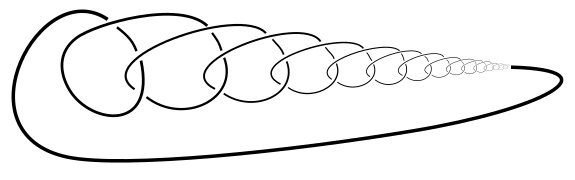
\includegraphics[scale=.6]{pics/Wild_knot}
\vskip0mm
\end{figure}
If one adds that the curve has to be smooth and regular,
then these examples disappear, but it is still a tricky to give right definition of \emph{deformation} --- the following diagram shows 
\begin{figure}[h]
\vskip-0mm
\centering
\includegraphics[scale=1]{pics/knot}
\vskip0mm
\end{figure}
that it can not be defined as a continuous family of closed simple smooth regular curves. 
Observe that all curves on the diagram are smooth and regular for all times including the last moment.

We define a \emph{knot} (more precicely \emph{tame knot}) as a simple closed polygonal line in Euclidean space~$\RR^3$.

The notation $\triangle abc$ is used for triangle $abc$; that is a polygonal line with three edges and vertexes $a$, $b$ and $c$.
Let us denote by $\solidtriangle abc$ the convex hull of the points $a$, $b$ and $c$; $\solidtriangle abc$ is the solid triangle with the vertexes $a$, $b$ and $c$.
The points $a$, $b$ and $c$ are assumed to be distinct, but they might lie on one line;
that is, for us a degenerate triangle is a triangle.

We understand a \emph{triangular isotopy} of a knot to be the generation of a new knot from the original one by means of the
following two operations:

Assume $[pq]$ is an edge of the knot and $x$
is a point such that the solid triangle $\solidtriangle pqx$  has no common points with the knot except for the edge $[pq]$.
Then we can replace the edge $[pq]$ in the knot by two adjacent edges $[px]$ and $[xq]$.

We can also perform the inverse operation.
That is, if for two adjacent edges $[px]$ and $[xq]$ of a knot the triangle
$\solidtriangle pqx$ has no common points with the knot except for the points on the edges $[px]$ and $[xq]$,
then we can replace two adjacent edges $[px]$ and $[xq]$ by one edge $[pq]$.

Polygons that arise from one another by a finite sequence of
triangular isotopies are called \emph{isotopic}.

\begin{wrapfigure}{r}{22 mm}
\vskip-4mm
\centering
\includegraphics{mppics/pic-18}
\vskip0mm
\end{wrapfigure}

A knot that is not isotopic to a triangle is called nontrivial.

The trefoil knot shown on the diagram gives a simple example of nontrivial knot.
A proof that the trefoil knot is nontrivial can be found in any textbook on knot theory, we do not give it here.
The most elementary and visual proof is based on the so called \emph{tricolorability} of knot diagrams.   

\begin{thm}{Exercise}\label{ex:triangle-isotopy}
Let $x$ and $y$ be two points on the adjacent edges $[p_1p_2]$ and $[p_2p_3]$ of a knot $\beta=p_1p_2p_3\dots p_n$.
Assume that the solid triangle $\solidtriangle xp_2y$ intersects $\beta$ only along the $[xp_2]\cup [p_2y]$.
Show that the knot $\beta'=p_1xyp_3\dots p_n$ is isotopic to $\beta$.
\end{thm}



\section{F\'ary--Milnor theorem}

We will give few proofs of the following theorem.

\begin{thm}{Theorem}\label{thm:fary-milnor}
The total curvature of any nontrival knot is at least $4\cdot\pi$. 
\end{thm}

The famous F\'ary--Milnor theorem states that the inequality is strict;
that is, the total curvature of any nontrival knot \emph{exceeds} $4\cdot\pi$.
It is easy to construct a trefoil knot with total curvature arbitrary close to $4\cdot\pi$;
therefore this result is optimal.

The question was raised by Karol Borsuk \cite{borsuk} and answered independently by Istv\'an F\'ary and John Milnor \cite{fary, milnor};
latter few other proofs were found.

\section{Milnor's proof}

In the proof we will use the following fact. 

\begin{thm}{Proposition}\label{prop:one-max-one-min}
Assume that a height function $(x,y,z)\to z$ 
has only one local minimum and one local maximum on a closed simple polygonal line and all the vertexes of the polygonal line lie on different height.
Then the line is a trivial knot.
\end{thm}

The proof is a simple application of the definition of isotopy, given in the previous section. 

\begin{wrapfigure}{r}{20 mm}
\vskip-0mm
\centering
\includegraphics{mppics/pic-19}
\vskip0mm
\end{wrapfigure}

\parit{Proof.}
Let $\beta=p_1\dots p_n$ be the closed simple polygonal line
such that the height function $(x,y,z)\to z$ has one local minimum one local maximum.
Note that on each of the two arcs of $\beta$ from min-vertex to max-vertex the height function increases monotonically.

Consider three vertexes with the largest value of the height function;
they have to include the max-vertex and two more.
Note that these three vertexes are consequent in the polygonal line; 
without loss of generality we can assume that they are $p_{n-1},p_n,p_1$.

Note that the solid triangle $\solidtriangle p_{n-1}p_np_1$ does not intersect any edge $\beta$ except the two adjacent edges $[p_{n-1}p_n]\cup[p_np_1]$.
Indeed, if $\solidtriangle p_{n-1}p_np_1$ intersects $[p_1p_2]$,
then, 
since $p_2$ lies below $\solidtriangle p_{n-1}p_np_1$,
$[p_1p_2]$ must intersect $[p_{n-1}p_n]$
which is impossible since $\beta$ is simple.
The same way one can show that $\solidtriangle p_{n-1}p_np_1$ can not intersect $[p_{n-2}p_{n-1}]$.
The remaining edges lie below $\solidtriangle p_{n-1}p_np_1$, hence they can not intersect this triangle.

Applying triangular isotopy, to $\solidtriangle p_{n-1}p_np_1$ we get a closed simple polygonal line $\beta'\z=p_1\dots p_{n-1}$ which is isotopic to $\beta$.

Since all the vertexes $p_i$ have different height,
the assumption of proposition holds for $\beta'$.

Repeating this procedure $n-3$ times we get a triangle.
Hence $\beta$ is a trivial knot.
\qeds

\parit{Milnor's proof of \ref{thm:fary-milnor}.}
Let $\alpha$ be a simple closed polygonal line.
Assume its total curvature is less that $4\cdot\pi$.
Then by Proposition~\ref{prop:tc-crofton}, 
\[\tc\alpha_u<4\cdot\pi\]
for some unit vector $u$.
Moreover, we can assume that $u$ points in a generic direction;
that is, $u$ is not perpendicular to any edge or diagonal of $\alpha$.

The total curvature of $\alpha_u$ is $\pi$ times the number of turns of $\alpha_u$
which has to be an even number.
It follows that number of turns of $\alpha_u$ is at most $2$;
it can not be less than 2 for generic direction and therefore it is $2$.

That is, if we rotate the space so that $u$ pints to the top,
than the height function has exactly one minimum and one maximum;
by Proposition~\ref{prop:one-max-one-min}, $\alpha$ is a trivial knot --- hence the result.
\qeds

\section{F\'ary's proof}

Let us give a sketch of another proof, based on the original idea of Istv\'an F\'ary.

\begin{wrapfigure}{r}{30 mm}
\vskip-0mm
\centering
\includegraphics{mppics/pic-13}
\vskip0mm
\end{wrapfigure}

\parit{F\'ary's proof of \ref{thm:fary-milnor}.}
Consider a projection of the knot to a plane in general position.
That is, we assume that the self-intersections of the projection are at most double and the projection of each edge does not degenerate.
The obtained closed polygonal line $\beta=p_1p_2\dots p_n$ divides the plane into domains, one of which is unbounded, denote it by $U$, and the others are bounded.

First note that all domains can be colored in a chessboard order;
that is, they can be colored in black and white in such a way that domains with common borderline get different colors.
If the unbounded domain gets white color and every other domain is black then one can untie the knot by flipping these domains one by one.

\begin{thm}{Exercise}
Give a formal proof of the last statement; that is, show that if only undbounded domain is white then $\beta$ is isotopic to a triangle. 
\end{thm}

\begin{wrapfigure}{r}{30 mm}
\vskip-4mm
\centering
\includegraphics{mppics/pic-14}
\vskip0mm
\end{wrapfigure}

Therefore among the bounded domains there is a white domain, denote it by $D$.
The domain $D$ can not have a borderline with $U$ since they have the same color.
Fix a point $o$ in this domain.

For each $i$, set 
\begin{align*}
\phi_i&=\pi-\measuredangle p_{i-1}p_ip_{i+1},
\\
\psi_i&=\measuredangle p_{i-1} o p_{i},
\\
\theta_i&=\measuredangle o p_i p_{i+1}.
\end{align*}
Here indexes are taken modulo $n$; in particular, $p_{n}=p_0$.


Note that $\phi_i$ is the external angle at $p_i$;
therefore 
\[\tc\beta= \phi_1+\dots+\phi_n\]

Direct calculations show that 
\[\phi_i\ge \psi_i+\theta_{i-1}-\theta_i.\]
In the two pictures below, $\phi_i$ is the solid angle;
the rest of angles $\psi_i$, $\theta_{i-1}$ and $\theta_i$
are the same.
We have equality on the first picture and strict inequality on the second picture.

\begin{figure}[h]
\vskip-0mm
\centering
\includegraphics{mppics/pic-15}
\vskip0mm
\end{figure}

It follows that 
\[\phi_1+\dots+\phi_n\ge \psi_1+\dots+\psi_n.\]

The last sum 
is the total angle at  which $\beta$ seen from $o$ counted with multiplicity. 
The boundary of $D$ contributes at least $2\cdot\pi$ to this sum and the boundary of $U$ contributes an other $2\cdot\pi$;
since their boundaries do not overlap we get 
\[\psi_1+\dots+\psi_n\ge 4\cdot\pi,\]
hence the result.

This is true for the projection of the knot to any plane in general position.
The remaining planes contribute nothing to the average value.
Therefore by Proposition~\ref{prop:tc-crofton}, the total curvature of the original knot is at least $4\cdot\pi$.
\qeds



\begin{thm}{Exercise}
Construct a closed smooth simple curve with total curvature arbitrary close to $2\cdot\pi$ such that its projection to any plane has at least $10$ self-intersections.   
\end{thm}



\section{Proof of Alexander and Bishop}

Here we sketch a proof of F\'ary--Milnor theorem given by of Stephanie Alexander and Richard Bishop in \cite{alexander-bishop}.

The proof is elementary, but not simple 
(elementary does not mean simple, it means only that it does not use much theory).
It is based on the following two facts that we already familiar with:
\begin{itemize}
\item If a closed polygonal line $\beta'$ is inscribed in a closed polygonal line $\beta$ then 
 \[\tc\beta'\le \tc\beta.\]
\item The total curvature of doubly covered
bigon is $4\cdot\pi$; that is,
\[\tc\beta=4\cdot\pi\]
if $\beta=pqpq$ for two distinct points $p$ and $q$.
Similarly if a quadrilateral is sufficiently close to a doubly covered
bigon, then its total curvature is close to $4\cdot\pi$.
\end{itemize}


\parit{Proof.}
Let $\beta=p_1\dots p_n$ be a closed polygonal line that is not a trivial knot;
that is, one can not get a triangle from $\beta$ by applying a sequence of triangular isotopys defined in the previous section.

We proceed by induction on the number $n \ge 3$.
In the base case $n=3$ the polygonal line $\beta$ is a triangle.
Therefore, by the definition, $\beta$ is a trivial knot --- nothing to prove.

Consider the smallest $n$ for which the statement fail;
that is, there is a closed simple polygonal line $\beta\z=p_1\dots p_n$ that is not a trivial knot such that
\[\tc\beta<4\cdot\pi.
\eqlbl{eq:<4pi}\]
We use the indexes modulo $n$ that is $p_0=p_n$, $p_1=p_{n+1}$ and so on.
Without loss of generality, we may assume that $\beta$ is in general position; 
that is, no four vertexes of $\beta$ lie on one plane. 

Set $\beta_0=\beta$.
If the solid triangle $\solidtriangle p_{0}p_1p_{2}$ intersects $\beta_0$ only by the two adjacent edges,
then applying the corresponding triangular isotopy, we get a knot $\beta'_0$ with $n-1$ edge that is inscribed in $\beta_0$ therefore
\[\tc\beta_0\ge \tc\beta_0'.\]
On the other hand by induction hypothesis 
\[\tc\beta_0'\ge 4\cdot\pi\]
which contradicts \ref{eq:<4pi}.

Choose the first point $w'_1$ on the edge $[p_1p_2]$ so that the line segment $[p_0w'_1]$ 
intersects $\beta_0$.
Denote a point of intersection by $y_1$.

\begin{wrapfigure}{r}{25 mm}
\vskip-0mm
\centering
\includegraphics{mppics/pic-17}
\vskip0mm
\end{wrapfigure}

Choose a point $w_1$ on $[p_1p_2]$ a bit before $w'_1$
(below we explain how close).
Denote by $x_1$ the point on $[p_0w_1]$ that minimize the distance to $y_1$.
This way we get a closed polygonal line 
$\beta_1\z=w_1p_2\dots p_n$ with two marked points $x_1$ and $y_1$.
Denote by $m_1$ the number of edges in the arc $y_1w_1\dots x_1$ of $\beta_1$.

By Exercise~\ref{ex:triangle-isotopy}, $\beta_1$ is isotopic to $\beta_0$;
in particular $\beta_1$ is a nontrivial knot.

Now let us repeat the procedure for the adjacent edges $[w_1b_2]$ and $[b_2b_3]$ of $\beta_1$.
If the solid triangle $\solidtriangle w_1b_2b_3$ intersects $\beta_1$ only at these two adjacent edges, then we get a contradiction with the induction hypothesis the same way as before.
Otherwise we get a new knot $\beta_2=w_1w_2b_3\dots b_n$ with two marked points $x_2$ and $y_2$.
Denote by $m_2$ the number of edges in the broken line $y_2w_3\dots x_2$.

Note that the points $x_1,x_2,y_1,y_2$ can not appear on $\beta_2$ in the same cyclic order;
otherwise the broken line $x_1x_2y_1y_2$ can be made to be arbitrary close to a doubly covered bigon which again contradicts~\ref{eq:<4pi}.%
\footnote{More precisely, the choice of $w_1$ has to be made so that the distance $|x_1-y_1|$ would be much less that all the distances between $y_1$ and any point $z\in\beta\cap \solidtriangle p_1p_2p_3$, so we have
\[\measuredangle y_1zx_1<\tfrac\eps{10},\]
where $\eps=4\cdot\pi-\tc\beta$.
In this case, since $y_2\in \beta\cap \solidtriangle p_1p_2p_3$ and $x_2$ can be taken arbitrary close to $y_2$, we have
\[\tc x_1x_2y_1y_2 > 4\cdot\pi -\eps= \tc\beta\]
which can not happen since $x_1x_2y_1y_2$ is inscribed in $\beta$.}

Therefore we can assume that the arc $x_2w_2\dots y_2$ lies inside of arc $x_1w_1\dots y_1$ in $\beta_2$
and therefore $m_1>m_2$.

Continuing this procedure we get a sequence of polygonal lines $\beta_i\z=w_1\dots w_i p_{i+1}p_n$ with marked points $x_i$ and $y_i$ such that the number of edges $m_i$ from $x_i$ to $y_i$ decreases in $i$.
Clearly $m_i>1$ for any $i$ and $m_1<n$.
Therefore it requires less than $n$ steps we get a contradiction with the induction hypothesis.
\qeds

\begin{wrapfigure}{r}{30 mm}
\vskip-0mm
\centering
\includegraphics{mppics/pic-20}
\vskip0mm
\end{wrapfigure}

\begin{thm}{Exercise}
Suppose that a closed curve $\alpha$ crosses a line at four points $a$, $b$, $c$ and $d$.
Assume that the points $a$, $b$, $c$ and $d$ appear on the line in the same order and they appear on the curve $\alpha$ in the order $a$, $c$, $b$, $d$.
Show that 
\[\tc\alpha\ge 4\cdot\pi.\]
\end{thm}

A line crossing a knot at four points as in the exercise is called \emph{alternating quadrisecants}.
It turns out that any nontrivial knot adits an alternating quadrisecants \cite{denne};
it provides yet an other proof of F\'ary--Milnor theorem.


\begin{thm}{Advanced exercise}
Show that given any real number $\Phi$ there is a knot $\beta$ such that any knot isotopic to $\beta$ has total curvature at least~$\Phi$.   
\end{thm}

\parit{Hint:} Use that there are knots with arbitrary large \emph{bridge number}, see for example \cite{schultens} and the references there in.



%\chapter{Convex surfaces}


\section{Positive Gauss curvature}
A set in $X$ Euclidean space is called strictly convex if for any two points $x,y\in X$ any point $z$ that lies between $x$ and $y$ lies in the interior of $X$.
Clearly any open convex set is stricly convex;
the cube (as well as any convex polyhedron) geves an example of convex set which is not strictly convex.

\begin{thm}{Exercise}\label{ex:loc-convex}
Let $\Sigma$ be a surface with positive Gauss curvature.
Show that for any point $p\in \Sigma$ and all sufficiently small $\eps>0$,
the surface $\Sigma$ divides the ball $B(p,\eps)$ into two regions, one of which is strictly convex.
\end{thm}

The following theorem gives a global version of the exercise above.

\begin{thm}{Theorem}
Assume $\Sigma$ is a closed smooth connected surface with positive Gauss curvature that bounds a bounded region $R$.
Then $R$ is convex and $\Sigma$ is a sphere; that is, $\Sigma$ admits a smooth regular parametrization by $\SS^2$.

\end{thm}

\parit{Proof.} Since $\Sigma$ is connected, so it $R$.
Moreover any two points $x$ and $y$ in the interior of $R$ can be connected by a polygonal line $\beta$ in the interior of $R$.

Arguing by contradiction, assume the line segment $[xy]$ does not lie in the   in the interior of $R$.
Let $y_0$ be the first point on $\beta$ so that the line segment $[xy_0]$ touches $\Sigma$; assume it touch it at a point $z$.

By Exercise \ref{ex:loc-convex}, $R\cap B(z,\eps)$ is strictly convex for all sufficiently small $\eps>0$.
On the other hand $z$ lies between two points common to the line segment $[xy_0]$ and $R\cap B(z,\eps)$ --- a contradiction.

It remains to parameterize $\Sigma$ by $\SS^2$.

Fix a point $p$ in the interior of $R$.
By strict convexity of $R$, for any point $x\in \SS^2$ there is unique point $x'\in \Sigma$ that lies on the halfline $px$;
moreover, the map $h\:x\mapsto x'$ describes a bijection $\SS^2\to \Sigma$.

Applying inverse function theorem in a local coordinates of $\SS^2$ and $\Sigma$,
we get that the map $h$ is smooth and regular.
Hence the result.
\qeds


\begin{thm}{Theorem}
Any closed connected immersed surface with positive Gauss curvature is embedded.
\end{thm}

\begin{wrapfigure}[8]{r}{20 mm}
\vskip-4mm
\centering
\includegraphics{mppics/pic-35}
\vskip0mm
\end{wrapfigure}

Note that an analogous statement does not hold in the plane;
on the diagram you see a closed curve with self-intersection and positive curvature at all points.


%\input{sol.tex}
%\chapter{Final exam}


\begin{enumerate}[A.]
\item Project presentaion.
\item One theoretical question:
\begin{enumerate}[1.]
\item Definition of length and its semicontinuity.
\item Axioms of length and Crofton's formula.
\item Formulations and variations of Crofton's formula.
\item Total curvature, Fenchel's theorem and equivalence of two definitions.
\item Knots and F\'ary--Milnor theorem; any proof.
\item Osculating circles and the spiral theorem.
\item Supporting circles and Four-vertex theorem. 
\item Moon in a puddle (Ionin--Pestov theorem).
\item Lagunov's example.
\item Hadamard--Stoker theorem (\ref{thm:convex-immersed}), any proof.
\item Liberman's lemma (\ref{lem:liberman}).
\item Usov's theorem (\ref{thm:usov}).
\item Gauss--Bonnet formula.
\item Cohn-Vossen theorem \ref{thm:cohn-vossen}.
\item Proposition~\ref{prop:loc-comp-l}.
\item Alexandrov's lemma.
\item Reformulations of comparison \ref{prop:comp-reformulations}.
\item Inheritance lemma
\item Toponogov comparison theorem (\ref{thm:comp}\textit{\ref{thm:comp:toponogov}}).
\item Cartan--Hadamard comparison theorem (\ref{thm:comp}\textit{\ref{thm:comp:cat}}).
\end{enumerate}

\item One exercise.

\item An additional problem for perfect score.
\end{enumerate}



%\input{tickets-tickets.tex}


\sloppy
\printbibliography[heading=bibintoc]
\fussy
\end{document}

\begin{thm}{Exercise}
Let $\gamma(t)$ be a smooth regular space curve.
Assume that there is function $|\gamma(t_1)-\gamma(t_2)|$ depends only on $t_2-t_1$;
that is there is a function $\ell$ such that $\ell(t_2-t_1)=|\gamma(t_1)-\gamma(t_2)|^2$ for any $t_1$ and $t_2$.
Show that 
\begin{enumerate}[(a)]
\item $2\cdot|\gamma'(t)|^2=\ell''(0)$;
\item $2\cdot|\gamma''(t)|^2=\ell^{(4)}(0)$;
\item $2\cdot|\gamma'''(t)|^2=\ell^{(6)}(0)$;
\item The vectors $\gamma'(t)$, $\gamma''(t)$, $\gamma'''(t)$ are orthogonal.
\item Conclude that $\gamma$ has constant curvature and torsion and therefor it is a helix (possibly degenerated to a line or circle). 
\end{enumerate}

\end{thm}
